\documentclass[UTF8,12pt]{article}
\usepackage{ctex}
\usepackage{indentfirst}
\usepackage{color}
\usepackage{hyperref}
\usepackage{graphicx}
\usepackage{subfigure}
\usepackage{pdfpages}
\usepackage{booktabs}
\usepackage{listings}
\hypersetup{
    hidelinks,
	colorlinks=true,
	allcolors=black,
	pdfstartview=Fit,
	breaklinks=true
}

\definecolor{dkgreen}{rgb}{0,0.6,0}
\definecolor{gray}{rgb}{0.5,0.5,0.5}
\definecolor{mauve}{rgb}{0.58,0,0.82}

\lstset{ %
  language=Octave,                % the language of the code
  basicstyle=\footnotesize,           % the size of the fonts that are used for the code
  numbers=left,                   % where to put the line-numbers
  numberstyle=\tiny\color{gray},  % the style that is used for the line-numbers
  stepnumber=2,                   % the step between two line-numbers. If it's 1, each line 
                                  % will be numbered
  numbersep=5pt,                  % how far the line-numbers are from the code
  backgroundcolor=\color{white},      % choose the background color. You must add \usepackage{color}
  showspaces=false,               % show spaces adding particular underscores
  showstringspaces=false,         % underline spaces within strings
  showtabs=false,                 % show tabs within strings adding particular underscores
  frame=single,                   % adds a frame around the code
  rulecolor=\color{black},        % if not set, the frame-color may be changed on line-breaks within not-black text (e.g. commens (green here))
  tabsize=2,                      % sets default tabsize to 2 spaces
  captionpos=b,                   % sets the caption-position to bottom
  breaklines=true,                % sets automatic line breaking
  breakatwhitespace=false,        % sets if automatic breaks should only happen at whitespace
  title=\lstname,                   % show the filename of files included with \lstinputlisting;
                                  % also try caption instead of title
  keywordstyle=\color{blue},          % keyword style
  commentstyle=\color{dkgreen},       % comment style
  stringstyle=\color{mauve},         % string literal style
  escapeinside={\%*}{*)},            % if you want to add LaTeX within your code
  morekeywords={*,...}               % if you want to add more keywords to the set
}


\setlength{\parindent}{2em}

\begin{document}



\begin{center}
    \tableofcontents
\end{center}
\newpage

\section{开发工具及环境说明}
\subsection{开发工具}
使用IntelliJ IDEA 2021.1.3集成开发环境,JDK版本为Java 17.0.4.1,使用Windows 11操作系统进行开发。

\subsection{环境说明}
采用Java SE 基础模块进行开发,项目的运行依赖JVM(Java Virtual Machine,Java虚拟机)

项目依赖的Jar包有:

\begin{itemize}
    \item jl1.0.jar
    \item mysql-connector-java-8.0.28.jar
\end{itemize}

分别用于录音功能和数据库连接。

在运行项目前,需要在运行环境中配置JVM,以及上述两个Jar包;数据库使用MySQL,需要提前建立好MySQL数据库login,并在其中建立好表client,使用NavicatPremium进行数据库的管理。
\newpage

\section{网络聊天程序业务分析}
\subsection{相关业务分析}
在网络聊天程序中,由客户端和服务器端两部分组成。在运行时,服务器端需要首先上线,开放端口,连接数据库和等待客户端连接。客户端需要连接服务器,连接成功后,可以进行登录、注册、聊天、查看聊天记录等操作。

\subsubsection{服务器端}
服务器端需要完成的功能有:
\begin{itemize}
    \item 上线,开放端口,连接数据库,等待客户端连接
    \item 接收客户端的连接请求,建立连接
    \item 接收客户端的登录请求,验证用户名和密码,返回登录结果
    \item 接收客户端的注册请求,验证用户名是否已存在,返回注册结果
    \item 接收客户端的聊天请求,将聊天内容按照对象转发,返回聊天内容
    \item 打印在线的客户端列表
    \item 实现远程强制下线功能,将指定客户端从在线列表中删除
    \item 实现群发功能,将聊天内容转发给所有在线客户端
\end{itemize}

综合上述服务器端炫耀实现的功能,服务器端的界面组成应该如下所示:
\begin{itemize}
    \item 服务器端的主界面,包含服务器的基本信息,以及在线客户端列表
    \item 消息输入框,用于群发消息的键入
    \item 群发消息按钮,用于发送群发消息
    \item 强制下线按钮,用于强制下线指定客户端
\end{itemize}

\subsubsection{客户端}
客户端需要完成的功能有:
\begin{itemize}
    \item 连接服务器,连接成功后,可以进行登录、注册、聊天、查看聊天记录等操作
    \item 弹出登录界面,可以选择登录或注册
    \item 注册功能,输入用户名和密码,发送注册请求,接收注册结果,在服务器端连接数据库查询用户名是否已存在,若不存在,则将用户名和密码插入数据库,返回注册成功;若存在,则返回注册失败
    \item 登录功能,输入用户名和密码,发送登录请求,接收登录结果,在服务器端连接数据库查询用户名和密码是否匹配,若匹配,则返回登录成功状态,并跳转聊天界面;若不匹配,则返回登录失败
    \item 公共聊天功能,输入聊天内容,发送聊天请求,接收聊天内容,在服务器端将聊天内容按照对象转发,返回聊天内容
    \item 发送语音功能,点击发送语音按钮,开始录音,点击停止录音按钮,结束录音,将录音文件发送给服务器端,服务器端将录音文件转发给所有在线客户端,客户端可自主选择是否播放录音
    \item 发送文件功能,点击发送文件按钮,选择文件,将文件发送给服务器端,服务器端将文件转发给所有在线客户端,客户端可自主选择是否下载文件
    \item 查看系统时间功能,点击查看系统时间按钮,向服务器端发送请求,服务器端返回系统时间
    \item 接收服务器端的强制下线请求,弹出提示框,提示用户被强制下线
    \item 接收服务器端的群发消息,在消息接受区域显示群发消息
    \item 私聊功能,选择私聊对象,发送私聊请求,如果对方接受私聊,则可以进行私聊,私聊内容只有私聊双方可见,在私聊窗口可以实现发送文字、发送语音、发送文件以及窗口抖动功能
    \item 主动退出功能,点击退出按钮,向服务器端发送退出请求,服务器端将客户端从在线列表中删除,客户端退出    
\end{itemize}

综合上述客户端需要实现的功能,客户端的界面组成应该如下所示:

\begin{itemize}
    \item 登录界面,包含用户名输入框、密码输入框、登录按钮、注册按钮
    \item 注册界面,包含用户名输入框、密码输入框、确认密码输入框、注册按钮、返回按钮、头像上传按钮
    \item 聊天界面,包含聊天内容显示区域、聊天输入框、发送消息按钮、发送语音按钮、发送文件按钮、查看系统时间按钮、退出按钮、在线用户列表、强制下线按钮
    \item 私聊界面,包含聊天内容显示区域、聊天输入框、发送语音按钮、发送文件按钮、窗口抖动按钮、退出按钮
\end{itemize}

接下来对客户端功能进行详细的说明:

当每个客户端进行连接时,会首先跳出登录界面;当用户是首次使用本系统时,可以进行注册,即点击“注册”按钮,客户端输入帐号、密码和确认密码进行注册。客户还可以选取自己的头像,当没有选择头像时,系统将会选用默认头像作为他的头像。当客户端提交注册信息时,服务器端将会进行以下的判断条件:若帐号被注册,则拒绝本次注册,否则判断密码和确认密码是否相同;若相同则同意本次注册,并将帐号和密码信息存储于数据库中;若不相同则拒绝本次注册。注册完的账户当进行再次登录系统时,无需注册,直接登录即可。客户端进行登录时,首先输入帐号和密码,并点击“登录”,服务器端通过数据库查询操作判断帐号是否存在、帐号和密码信息是否对应,若存在并对应,再判断用户是否重复登录,若非重复登录则同意登录,开放文件传输端口并与客户端连接,同时将帐号和ChatThread类对象的对应关系记录于HashMap中,以便后续添加、删除成员和聊天记录的转发,否则任意一种情况都将拒绝登录。

当客户端进行语音聊天时,客户端点击“发送语音”按钮,将弹出录音窗口,点击“开始录音”;当客户端点击“结束录音”时,客户端将会把帐号和录音文件发送到服务器端;服务器端接收录音,并将录音转发给除了录音客户端以外的其他客户端,客户端接收录音后,会弹出“[语音接收提醒]”,并选择是否接收;若同意接收,则会播放服务器端传入的由录音客户端发来的语音,否则将会丢弃该语音。

当客户端进行传送文件时,客户端点击“发送文件”按钮,客户端会选取系统中的文件并发送给服务器,服务器端将文件转发给除了发送文件客户端以外的其他客户端,客户端接收文件后,会弹出“[文件接收提醒]”,并选择是否接收;若同意接收,则会打开服务器端传入的由文件客户端发来的文件,否则将会丢弃该文件,文件的类型可为txt、pdf、docx等。

当客户端想要查看系统时间时,点击“系统时间”按钮即可,可以校对系统时间;当客户端想要离开聊天室时,点击“离开聊天室”,客户端将会给服务器发送离开聊天室的标记,服务器接收到后会同意请求,并为其他各客户端发送其离开聊天室的记录,客户端会将其显示在聊天记录框中。

\newpage

\subsection{相关业务流程图}
\subsubsection{注册登录流程图}
\begin{figure}[htbp]
    \centering
    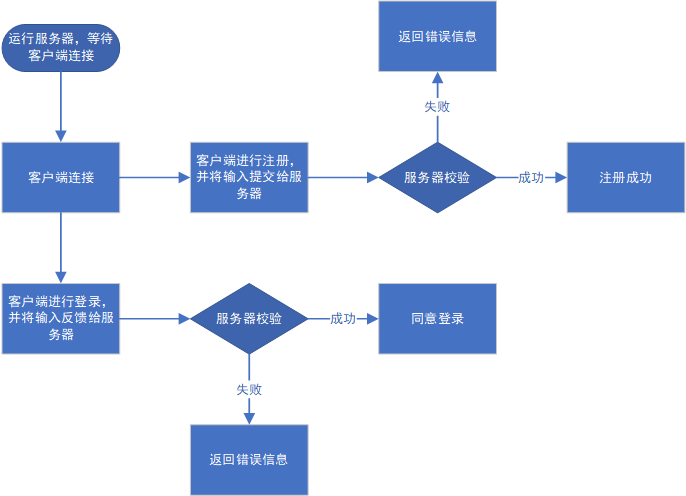
\includegraphics[width=0.6\textwidth]{img/1.png}
    \caption{注册登录流程图}
\end{figure}

\subsubsection{语音聊天流程图}
\begin{figure}[htbp]
    \centering
    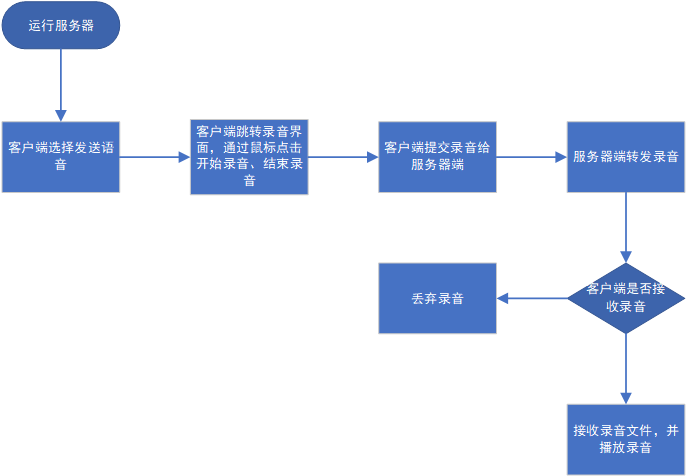
\includegraphics[width=0.6\textwidth]{img/2.png}
    \caption{语音聊天流程图}
\end{figure}

\subsubsection{文件传输流程图}
\begin{figure}[htbp]
    \centering
    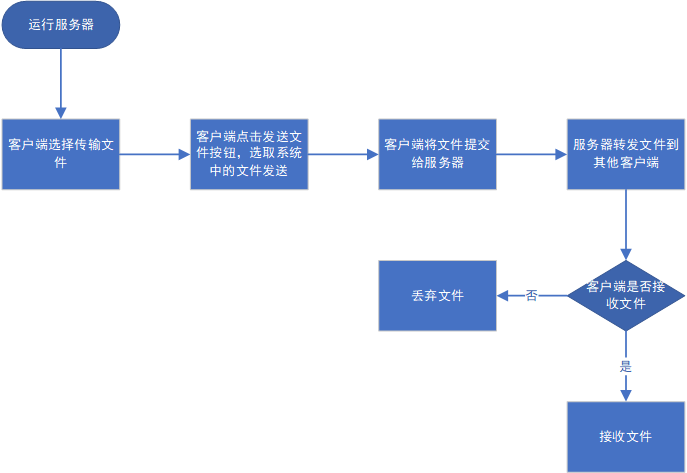
\includegraphics[width=0.6\textwidth]{img/3.png}
    \caption{文件传输流程图}
\end{figure}

\subsubsection{主动离开聊天室流程图}
\begin{figure}[htbp]
    \centering
    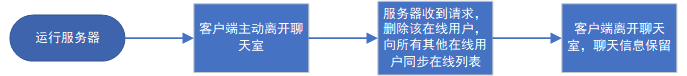
\includegraphics[width=0.6\textwidth]{img/4.png}
    \caption{主动离开聊天室流程图}
\end{figure}

\subsubsection{强制下线流程图}
\begin{figure}[htbp]
    \centering
    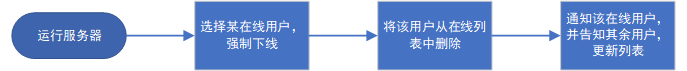
\includegraphics[width=0.6\textwidth]{img/5.png}
    \caption{强制下线流程图}
\end{figure}

\newpage

\section{网络聊天程序系统设计}
\subsection{系统功能定义}
\begin{enumerate}
    \item 用java图形界面编程编写客户端和服务器端程序,实现客户端和服务器端的交互,支持多客户端同时在线聊天,且连接到同一个服务器端,每个客户端都能够进行登录或者注册,初始界面为登录界面。
    \item 可以实现群聊,即公共聊天室,所有在线的客户端都能够看到聊天室中的聊天内容,可以发送文字、语音、文件,可以查看系统时间,可以退出聊天室。
    \item 在服务器端,完成在线用户列表的显示,可以查看当前在线的用户,可以实现强制下线功能,可以实现群发功能;在客户端,完成在线用户列表的显示,可以查看当前在线的用户,双击用户可以进行私聊。
    \item 可以实现私聊,即私人聊天室,只有两个用户能够看到聊天内容,可以发送文字、语音、文件,可以发送窗口抖动,可以退出聊天室。
    \item 客户端的上线下线能够实时更新到服务器端,服务器端的上线下线能够实时更新到客户端。
\end{enumerate}

\subsection{消息头部设计}
客户端与服务器端之间的通信,需要通过消息头部来进行标识,通过对客户端提交信息的划分,获取头部信息,从而得知信息类别,进行相应的操作。

消息头部设计如下:

\begin{tabular}{cc}
    \toprule
    消息头部 & 具体含义 \\
    \midrule
    REG1&检查注册时密码和确认密码一致性\\
    YES&注册密码和确认密码一致\\
    NO&注册信息有误或登录信息有误\\
    REG2&检查注册时用户名是否已经被注册\\
    EXISTS&用户名已经存在\\
    INSERT&用户名已经成功注册\\
    LOGIN&用户登录\\
    CHONG&用户重复登录,登录失败\\
    NO&用户不存在或输入信息不正确,登录失败\\
    NEW&新用户登入聊天室\\
    USER&服务器发送好友列表\\
    RUN&客户端离开聊天室\\
    SILIAO&客户端请求私聊\\
    ACCEPT/REFUSE&同意/拒绝私聊\\
    SI&客户端发送私聊消息\\
    SIMESSAGE&服务器转发的客户端私聊消息\\
    SID&发送私聊窗口抖动\\
    \bottomrule
\end{tabular}

\subsection{服务器端设计}
\subsubsection{服务器端的界面设计}
服务器的界面主要由两部分组成,分别是在线客户列表和服务器功能实现区,即群发消息、强制下线等功能的实现区。

以下是界面对象的定义:
\begin{lstlisting}[title=界面对象的定义,frame=shadowbox]
    private JLabel explain = new JLabel("在线用户列表",JLabel.CENTER);
    private List users = new List();
    private JScrollPane listPane = new JScrollPane(users);       //设置滚动视图
    private JButton jbt = new JButton("远程关闭");
    private JButton Send_Button = new JButton("群发消息");
    private JTextField Sendword = new JTextField(20);       //发文字区域
    private ServerSocket ss = null;
    private Font font = new Font("微软雅黑", Font.BOLD, 25);
\end{lstlisting}

以下是界面的初始化代码:

\begin{lstlisting}[title=服务器界面的初始化,frame=shadowbox]
    public Server() throws Exception{
        this.setLayout(null);
        Class.forName("com.mysql.cj.jdbc.Driver");     //Class.forName查找并加载指定的类,加载数据库连接驱动并连接
        con = DriverManager.getConnection(url,user,pass);

        explain.setLocation(0,0);
        explain.setSize(430,50);
        explain.setFont(font);

        listPane.setLocation(0,50);
        listPane.setSize(430,320);

        users.setFont(new Font("Consolas", Font.PLAIN, 25));

        Sendword.addActionListener(this);
        Sendword.setLocation(0,370);
        Sendword.setSize(250,57);
        Sendword.setFont(new Font("微软雅黑", Font.PLAIN, 25));

        jbt.addActionListener(this);
        jbt.setSize(90,56);
        jbt.setLocation(250,370);
        jbt.setFont(new Font("微软雅黑", Font.PLAIN, 13));
        jbt.addActionListener(this);

        Send_Button.addActionListener(this);
        Send_Button.setSize(90,56);
        Send_Button.setLocation(340,370);
        Send_Button.setFont(new Font("微软雅黑", Font.PLAIN, 13));

        this.setTitle("服务器");
        this.add(explain);
        this.add(listPane);
        this.add(jbt);
        this.add(Sendword);
        this.add(Send_Button);
        this.setDefaultCloseOperation(EXIT_ON_CLOSE);
        this.setSize(435,465);
        this.setVisible(true);

        ss = new ServerSocket(9999);    //信息传送使用端口
        new Thread(this).start();
    }
\end{lstlisting}

在界面初始化的过程中,同时绑定了端口9999,用于信息传送;还调用了数据库连接驱动,连接到数据库,以便后续的数据库操作。

\subsubsection{远程关闭和群发消息功能的实现}

对于两个按钮“远程关闭”、“群发消息”,分别绑定了事件监听器,用于实现相应的功能。事件监听器的实现代码如下:

\begin{lstlisting}[title=事件监听器的实现,frame=shadowbox]
    public void actionPerformed(ActionEvent e){
        if(e.getSource() == jbt){
            //远程关闭按钮
            Leave(1,null);
        }else if(e.getSource() == Sendword || e.getSource() == Send_Button){
            //群发消息按钮
            for(String ct : users_connect.keySet()){    //利用key值遍历哈希表
                users_connect.get(ct).Send.println("系统消息 "+new SimpleDateFormat("yyyy-MM-dd HH:mm:ss").format(new Date()));
                users_connect.get(ct).Send.println(Sendword.getText());
            }
            Sendword.setText("");       //清空输入框
        }
    }
\end{lstlisting}

其中,远程关闭功能通过调用Leave函数实现,群发消息功能通过遍历哈希表,将消息发送给所有在线客户端实现。

\subsubsection{客户端离开功能的实现}
离开功能通过Leave函数实现,在本实验中,离开有两种情况:
\begin{itemize}
    \item 客户端主动离开
    \item 服务器端强制下线
\end{itemize}
两种下线操作会对某一用户端发送不同消息,因此需要对两种情况进行区分,区分的方法是通过传入的参数来判断,参数为1时,表示服务器端强制下线,参数为0时,表示客户端主动离开。剩余操作两种情况几乎一致:
\begin{itemize}
    \item 从哈希表中删除该用户
    \item 用户列表中删除该用户
    \item 更新在线客户端用户列表及服务器端用户列表
\end{itemize}

Leave函数的实现代码如下:
\begin{lstlisting}[title=Leave函数的实现,frame=shadowbox]
    public void Leave(int num,String selectedUser){
        if(num == 1){
            selectedUser = users.getSelectedItem();
        }
        String msg = "LOGOUT-"+num+"-"+selectedUser;        //1是服务器t的,0是自己主动走的
        ChatThread ct = users_connect.get(selectedUser);
        ct.Send.println(msg);
        users.remove(selectedUser);
        users_connect.remove(selectedUser);
    }
\end{lstlisting}

\subsubsection{服务器端的主线程实现}
在服务器端最重要的就是服务器端的主线程,就是聊天线程,在本次实验中,将聊天和文件发送及录音发送做了业务切割,录音从本质上来说就是文件发送,因此将文件和录音的发送放在一个线程。

主线程主要实现的是
\begin{itemize}
    \item 客户端的登录请求,进行匹配校验、重复登录校验
    \item 客户端的注册请求,进行用户名是否存在的校验、密码和确认密码是否一致的校验
    \item 客户端的离线请求,进行在线用户的删除
    \item 客户端的私聊请求,等待目标客户端的接受或拒绝
    \item 客户端的公共消息转发
    \item 客户端的私聊消息转发
    \item 客户端的私聊窗口抖动
    \item 客户端的上线消息广播
    \item 客户端的下线消息广播
\end{itemize}

接下来对主线程实现的功能进行逐一拆分,首先需要将服务器端收到的消息依据分隔符“-”进行消息切割,获取消息头部,从而进行相应的操作。

\paragraph{客户端的注册请求}

当用户收到注册的请求中的密码和确认密码是否一致的请求时,服务器端需要对密码和确认密码进行校验,校验的代码如下:
\begin{lstlisting}[title=确认密码校验,frame=shadowbox]
    if(msgs[0].equals("REG1")){
                        if(msgs[1].equals(msgs[2])){
                            Send.println("YES");
                        }else{
                            Send.println("NO");
                        }
    }
\end{lstlisting}

当用户收到注册的请求中的用户名是否存在的请求时,服务器端需要对用户名是否存在进行校验。如果校验通过,则将用户名和密码以及头像插入数据库,否则返回用户名已存在的消息。在这当中,需要查询数据库,因此需要用到SQL语句。校验的代码如下:

\begin{lstlisting}[title=用户名是否存在校验,frame=shadowbox]
    else if(msgs[0].equals("REG2"))
    {
        try{
            String sql = "select username from client where username=?";  //?为占位符
            PreparedStatement ptmt = con.prepareStatement(sql);     //加入预编译语句
            ptmt.setString(1,msgs[1]);  //1是ID
            ResultSet rs = ptmt.executeQuery();
            if(rs.next()){
                Send.println("EXISTS");
            }else{
                Send.println("INSERT");
                sql = "insert into client (username,password,picture_path) values(?,?,?)";  //?为占位符
                ptmt = con.prepareStatement(sql);     //加入预编译语句
                ptmt.setString(1,msgs[1]);
                ptmt.setString(2,msgs[2]);
                ptmt.setString(3,msgs[3]);
                ptmt.execute();     //执行sql语句
                ptmt.close();
            }
        }catch(Exception exce){}
    }
\end{lstlisting}

\paragraph{客户端的登录请求}
客户端在登录请求的时候,发送的消息头部为“LOGIN”,服务器端需要对用户名和密码进行校验,检验完成后还需要对用户是否重复登录进行校验:
\begin{itemize}
    \item 用户名和密码校验:服务器端需要连接数据库,查询用户名和密码是否匹配,如果匹配则进入下一步校验操作,否则返回登录失败的消息
    \item 用户重复登录校验:服务器端需要遍历哈希表,判断该用户是否已经登录,如果已经登录,则返回重复登录的消息,否则将用户添加到哈希表中,并返回登录成功的消息
\end{itemize}

首先是用户名和密码校验的实现代码:
\begin{lstlisting}[title=用户名和密码校验,frame=shadowbox]
    String sql= "select username,password,picture_path from client where username=? and password=?";
    PreparedStatement ptmt = con.prepareStatement(sql);
    ptmt.setString(1,msgs[1]);
    ptmt.setString(2,msgs[2]);
    ResultSet rs = ptmt.executeQuery();
\end{lstlisting}

然后是用户重复登录校验的实现代码:
\begin{lstlisting}[title=用户重复登录校验,frame=shadowbox]
    if(rs.next()) {      //存在此人
    String path = rs.getString(3);
    for (String ct : users_connect.keySet()) {
        if(msgs[1].equals(ct)){  //是否重复登录
            Send.println("CHONG");
            chongfu = false;
            break;
        }
    }
    if(chongfu) {      //未重复
        Send.println("OK-"+path);     //同意登录
        NickName = msgs[1];
        users.add(NickName);
        users_connect.put(NickName, this);
        ServerFileThread serverFileThread = new ServerFileThread();  //服务器文件读写进程启动
        serverFileThread.start();
    }else{
        chongfu = true;  //将重复标记重新设置为true
    }
}else{      //拒绝登录
    Send.println("NO");
}
\end{lstlisting}

\paragraph{客户端的离线请求}
客户端的主动离线实现比较简单,通过遍历哈希表,向所有在线客户端发送离线消息,然后发送离线消息头。

\begin{lstlisting}[title=客户端的离线请求,frame=shadowbox]
    else if(msgs[0].equals("RUN")){
        for(String ct : users_connect.keySet()){    //利用key值遍历哈希表
            users_connect.get(ct).Send.println("系统消息 "+new SimpleDateFormat("yyyy-MM-dd HH:mm:ss").format(new Date()));
            users_connect.get(ct).Send.println("SLOGOUT-"+msgs[1]);
        }
    }
\end{lstlisting}

\paragraph{客户端的私聊请求}
用户发送私聊请求后,服务器只需要进行简单转发就可以了,主要关注点在于目标客户端的接受或拒绝,因此需要对目标客户端的接受或拒绝请求进行解析:
\begin{itemize}
    \item 接受请求:接收方显示发出方,然后发出方显示接收方聊天窗口
    \item 拒绝请求:发出方显示拒绝信息
\end{itemize}

\begin{lstlisting}[title=客户端的私聊请求,frame=shadowbox]
    else if(msgs[0].equals("SILIAO")){
        users_connect.get(msgs[1]).Send.println("SI-"+NickName);
    }else if(msgs[0].equals("ACCEPT")) {
        users_connect.get(NickName).Send.println("JIESHOU-" + msgs[1]); //接受方显示对方
        users_connect.get(msgs[1]).Send.println("JIESHOU-" + NickName); //发出方显示接受方
    }else if(msgs[0].equals("REFUSE")){
        users_connect.get(msgs[1]).Send.println("JUJUE-"+NickName);
    }
\end{lstlisting}

\paragraph{客户端的私聊消息的转发}
确定了私聊关系后,客户端发送的私聊内容需要进行转发,需要对消息头进行解析,然后进行相应的操作。

\begin{lstlisting}[title=客户端的私聊消息的转发,frame=shadowbox]
    else if(msgs[0].equals("SI")){
        //1为发送方,2为接收方,3为文字
        users_connect.get(msgs[2]).Send.println("SIMESSAGE-"+msgs[1]+"-"+msgs[3]);
        //自己也显示自己发了这个消息
        users_connect.get(msgs[1]).Send.println("SIMESSAGE-"+msgs[1]+"-"+msgs[3]);
    }
\end{lstlisting}

\paragraph{客户端的私聊窗口抖动}
客户端发送的私聊窗口抖动的消息头为“SID”,服务器端只需要对消息头进行解析,然后进行相应的操作即可。

\begin{lstlisting}[title=客户端的私聊窗口抖动,frame=shadowbox]
    else if(msgs[0].equals("SID")){
        users_connect.get(msgs[2]).Send.println("SIMESSAGE-"+msgs[1]+"-"+"[窗口抖动提醒]我发送了一条窗口抖动。");
        users_connect.get(msgs[2]).Send.println("SID");
        //自己也显示自己发了这个消息
        users_connect.get(msgs[1]).Send.println("SIMESSAGE-"+msgs[1]+"-"+"[窗口抖动提醒]我发送了一条窗口抖动。");
    }
\end{lstlisting}

\paragraph{客户端的上线消息广播}
客户端的上线消息广播需要对哈希表进行遍历,服务器端群发消息,向所有在线客户端发送上线消息,同时根据系统时间的早中午晚,客制化上线消息的格式。

\begin{lstlisting}[title=客户端的上线消息广播,frame=shadowbox]
    else if(msgs[0].equals("NEW")){
        Calendar c = Calendar.getInstance();
        for (String ct : users_connect.keySet()) {    //利用key值遍历哈希表
            users_connect.get(ct).Send.println("系统消息 " + new SimpleDateFormat("yyyy-MM-dd HH:mm:ss").format(new Date()));
            c.get(Calendar.HOUR_OF_DAY);
            if (c.get(Calendar.HOUR_OF_DAY) <= 5 || c.get(Calendar.HOUR_OF_DAY) >= 18)
                users_connect.get(ct).Send.println("SLOGIN-EVE-" + NickName);
            else if (c.get(Calendar.HOUR_OF_DAY) >= 6 && c.get(Calendar.HOUR_OF_DAY) <= 10)
                users_connect.get(ct).Send.println("SLOGIN-MOR-" + NickName);
            else if (c.get(Calendar.HOUR_OF_DAY) >= 14 && c.get(Calendar.HOUR_OF_DAY) <= 17)
                users_connect.get(ct).Send.println(("SLOGIN-AFT-" + NickName));
            else
                users_connect.get(ct).Send.println("SLOGIN-MOO-" + NickName);
            if (!ct.equals(NickName)) {
                Send.println("USER-" + ct);       //服务器发送之前的好友列表
            }
        }
    }
\end{lstlisting}

\paragraph{客户端的下线消息广播}
客户端的下线消息广播需要对哈希表进行遍历,服务器端群发消息,向所有在线客户端发送下线消息。

\begin{lstlisting}[title=客户端的下线消息广播,frame=shadowbox]
    else if(msgs[0].equals("RUN")){
        for(String ct : users_connect.keySet()){    //利用key值遍历哈希表
            users_connect.get(ct).Send.println("系统消息 "+new SimpleDateFormat("yyyy-MM-dd HH:mm:ss").format(new Date()));
            users_connect.get(ct).Send.println("SLOGOUT-"+msgs[1]);
        }
    }
\end{lstlisting}

\paragraph{客户端的公共消息转发}
在上述所有头部都不匹配的情况下,服务器端将会将消息转发给所有在线客户端,实现公共消息的转发。通过遍历哈希表,将消息转发给所有在线客户端。

\begin{lstlisting}[title=客户端的公共消息转发,frame=shadowbox]
    else{   //普通消息发送
    for(String ct : users_connect.keySet()){    //利用key值遍历哈希表
        users_connect.get(ct).Send.println(msgs[0]+" "+new SimpleDateFormat("yyyy-MM-dd HH:mm:ss").format(new Date()));
        users_connect.get(ct).Send.println(msgs[1]);
    }
}
\end{lstlisting}

至此,服务器端的主线程实现完毕,同时服务器端的主要功能实现完毕。

\subsection{客户端设计}
\subsubsection{客户端的界面设计}
客户端的界面主要由三部分组成,分别是登录界面、注册界面和聊天界面。三者的逻辑关系是:运行客户端之后,首先弹出登录界面,如果用户没有注册,则可以点击“注册”按钮,跳转到注册界面,注册完成后,可以点击“返回”按钮,跳转到登录界面,进行登录操作;如果用户已经注册,则可以直接进行登录操作,登录成功后,跳转到聊天界面,进行聊天操作。

首先对登录界面进行设计,登录界面主要由用户名输入框、密码输入框、登录按钮、注册按钮组成,界面对象的定义如下:
\begin{lstlisting}[title=登录界面对象的定义,frame=shadowbox]
    private JTextField Id = new JTextField(20);
    private JPasswordField Passwd =new JPasswordField(20);
    private JLabel welcome = new JLabel("JIANG聊",JLabel.CENTER);
    private JLabel zhanghao = new JLabel("账号:");
    private JLabel mima = new JLabel("密码:");
    private JLabel Picture = new JLabel();
    private JButton Login_Button = new JButton("登录");
    private JButton Register_Button = new JButton("注册");
\end{lstlisting}

然后对登录界面进行初始化,初始化代码如下:
\begin{lstlisting}[title=登录界面的初始化,frame=shadowbox]
    public Login() throws Exception{
        this.setLayout(null);

        Font font = new Font("微软雅黑", Font.PLAIN, 25);

        welcome.setLocation(20,50);
        welcome.setSize(600,80);
        welcome.setFont(new Font("微软雅黑", Font.BOLD, 45));

        Id.setLocation(250,200);
        Id.setSize(300,60);
        Id.setFont(font);

        Passwd.setLocation(250,300);
        Passwd.setSize(300,60);
        Passwd.setFont(font);

        zhanghao.setLocation(180,190);
        zhanghao.setSize(200,80);
        zhanghao.setFont(new Font("微软雅黑", Font.BOLD, 25));

        mima.setLocation(180,290);
        mima.setSize(200,80);
        mima.setFont(new Font("微软雅黑", Font.BOLD, 25));

        ImageIcon image = new ImageIcon("people.png");  //将图片路径作为参数传入
        image.setImage(image.getImage().getScaledInstance(100,100,Image.SCALE_DEFAULT));  //创建缩放版本图像

        Picture = new JLabel(image);
        Picture.setLocation(60, 230);
        Picture.setSize(100, 100);

        Register_Button.setLocation(120,400);
        Register_Button.setSize(160,60);
        Register_Button.setFont(font);
        Register_Button.addActionListener(this);

        Login_Button.setLocation(300, 400);
        Login_Button.setSize(160,60);
        Login_Button.setFont(font);
        Login_Button.addActionListener(this);

        //创建socket使用9999端口
        Socket s = new Socket("localhost", 9999);
        out = s.getOutputStream();
        ps = new PrintStream(out);
        br = new BufferedReader(new InputStreamReader(s.getInputStream()));

        //窗体基本设置
        this.add(welcome);
        this.add(Id);
        this.add(Picture);
        this.add(Passwd);
        this.add(zhanghao);
        this.add(mima);
        this.add(Login_Button);
        this.add(Register_Button);
        this.setTitle("欢迎登录");
        this.setLocation(200,100);
        this.setSize(600,550);
        this.setDefaultCloseOperation(EXIT_ON_CLOSE);
        this.setVisible(true);
    }
\end{lstlisting}

其中,socket的端口号为9999,与服务器端的端口号相同,用于信息传送;同时,还需要对输入输出流进行初始化,以便后续的信息传送;此外,还需要对图片进行缩放,以便在界面中显示。

\subsubsection{客户端的注册界面设计}
客户端的注册界面主要由用户名输入框、密码输入框、确认密码输入框、注册按钮、返回按钮、头像上传组成,界面对象的定义如下:

\begin{lstlisting}[title=注册界面对象的定义,frame=shadowbox]
    private JTextField Id = new JTextField(20);
    private JPasswordField Passwd =new JPasswordField(20);
    private JPasswordField querenPasswd =new JPasswordField(20);
    private static Connection con;              //建立连接
    private JLabel welcome = new JLabel("极致体验,就差一步。",JLabel.CENTER);
    private JLabel zhanghao = new JLabel("账号:");
    private JLabel mima = new JLabel("密码:");
    private JLabel querenmima = new JLabel("确认密码:");
    private JLabel tip = new JLabel("选取头像");
    private JButton Zhuce_Button = new JButton("注册");
    private JButton Pic_acquire = new JButton();
    private FileDialog dialog = null;
\end{lstlisting}

其中,设置一个FileDialog对象,用于选择头像文件,文件的限制是图片类型。

接下来是对注册界面的初始化,初始化代码如下:
\begin{lstlisting}[title=注册界面的初始化,frame=shadowbox]
    public Register(PrintStream ps, BufferedReader br) throws Exception{
        this.ps = ps;
        this.br = br;
        this.setLayout(null);

        Font font = new Font("微软雅黑", Font.PLAIN, 25);

        welcome.setLocation(20,50);
        welcome.setSize(600,80);
        welcome.setFont(new Font("微软雅黑", Font.BOLD, 45));

        Id.setLocation(290,200);
        Id.setSize(300,50);
        Id.setFont(font);

        Passwd.setLocation(290,260);
        Passwd.setSize(300,50);
        Passwd.setFont(font);

        querenPasswd.setLocation(290,320);
        querenPasswd.setSize(300,50);
        querenPasswd.setFont(font);

        zhanghao.setLocation(180,190);
        zhanghao.setSize(200,60);
        zhanghao.setFont(new Font("微软雅黑", Font.BOLD, 25));

        mima.setLocation(180,250);
        mima.setSize(200,60);
        mima.setFont(new Font("微软雅黑", Font.BOLD, 25));

        querenmima.setLocation(180,310);
        querenmima.setSize(200,60);
        querenmima.setFont(new Font("微软雅黑", Font.BOLD, 25));

        ImageIcon image = new ImageIcon("people.png");  //将图片路径作为参数传入
        image.setImage(image.getImage().getScaledInstance(100,100,Image.SCALE_DEFAULT));  //创建缩放版本图像

        Pic_acquire.setIcon(image);
        Pic_acquire.setLocation(60, 230);
        Pic_acquire.setSize(100,100);
        Pic_acquire.setFont(font);
        Pic_acquire.addActionListener(this);

        tip.setLocation(75,310);
        tip.setSize(200,80);
        tip.setFont(new Font("微软雅黑", Font.PLAIN, 15));

        Zhuce_Button.setLocation(200, 400);
        Zhuce_Button.setSize(200,60);
        Zhuce_Button.setFont(font);
        Zhuce_Button.addActionListener(this);

        //窗体基本设置
        this.add(welcome);
        this.add(Id);
        this.add(Passwd);
        this.add(querenPasswd);
        this.add(zhanghao);
        this.add(mima);
        this.add(querenmima);
        this.add(Zhuce_Button);
        this.add(Pic_acquire);
        this.add(tip);
        this.setTitle("欢迎注册");
        this.setLocation(200,100);
        this.setSize(620,550);
        this.setVisible(true);
    }
\end{lstlisting}

其中,需要对图片进行缩放,以便在界面中显示。

\subsubsection{客户端的聊天界面设计}
客户端的聊天界面主要由在线用户列表、聊天信息显示区、聊天信息输入区、发送按钮、发送文件按钮、发送语音按钮、发送窗口抖动按钮、退出按钮、查看系统时间按钮组成,界面对象的定义如下:

\begin{lstlisting}[title=聊天界面对象的定义,frame=shadowbox]
    private JScrollPane jsp = new JScrollPane();//滚动条
    private JButton Send = new JButton("发送文字");
    private JButton Send_Record = new JButton("发送语音");
    private JButton Send_File = new JButton("发送文件");
    private JButton myClock = new JButton("系统时间");
    private JButton Leave = new JButton("离开聊天室");
    private DefaultListModel<String> user = new DefaultListModel<String>();  //用户列表
    private JList<String> userList = new JList<String>(user);   //展示用户列表
    private JScrollPane listPane = new JScrollPane(userList);       //设置滚动视图
    private JTextField Sendword = new JTextField(20);       //发文字区域
    private JTextArea Chat = new JTextArea(10,45);     //聊天记录显示
    private JLabel myself = new JLabel("",JLabel.CENTER);
    private JLabel friend_list = new JLabel("好友列表",JLabel.CENTER);
\end{lstlisting}

其中,需要对聊天信息显示区、在线用户列表、聊天信息输入区进行滚动视图的设置,以便在信息过多的时候,可以进行滚动查看。

接下来是对聊天界面的初始化,初始化代码如下:
\begin{lstlisting}[title=聊天界面的初始化,frame=shadowbox]
    public Chat(String Nick,String path,PrintStream ps,BufferedReader br,OutputStream out) throws Exception{
        this.ps = ps;
        this.br = br;
        this.path = path;
        this.out = out;

        ps.println("NEW");
        Font font = new Font("微软雅黑", Font.PLAIN, 15);

        //设置Chat区域
        Chat.setFont(font);
        Chat.setLineWrap(true);         //设置自动换行
        Chat.setLocation(0,0);
        Chat.setEditable(false);        //聊天记录无法编辑
        Chat.setMargin(new Insets(7, 7, 7, 7));     //设置7mm边距

        JScrollPane jsp = new JScrollPane(Chat);         //设置一个滚动条
        jsp.setBounds(0,0,500,500);

        //设置控件位置
        Sendword.setLocation(0,500);
        Sendword.setSize(300,60);
        Sendword.setFont(font);

        Send.addActionListener(this);
        Send.setSize(95,60);
        Send.setLocation(300,500);
        Send.setFont(font);
        Send.setMargin(new Insets(0,0,0,0));   //设置按钮边框和标签之间空白为0

        myClock.addActionListener(this);
        myClock.setSize(85,69);
        myClock.setLocation(500,360);
        myClock.setFont(font);
        myClock.setBackground(new Color(255,255,204));          //设置按钮颜色为淡黄
        myClock.setMargin(new Insets(0,0,0,0));   //设置按钮边框和标签之间空白为0

        Send_Record.addActionListener(this);
        Send_Record.setSize(95,60);
        Send_Record.setLocation(395,500);
        Send_Record.setFont(font);
        Send_Record.setMargin(new Insets(0,0,0,0));   //设置按钮边框和标签之间空白为0

        Send_File.addActionListener(this);
        Send_File.setSize(95,60);
        Send_File.setLocation(490,500);
        Send_File.setFont(font);
        Send_File.setMargin(new Insets(0,0,0,0));   //设置按钮边框和标签之间空白为0

        Leave.addActionListener(this);
        Leave.setSize(85,69);
        Leave.setLocation(500,429);
        Leave.setFont(font);
        Leave.setMargin(new Insets(0,0,0,0));   //设置按钮边框和标签之间空白为0
        Leave.setBackground(new Color(255,255,204));          //设置按钮颜色为淡黄

        listPane.setSize(86,220);
        listPane.setLocation(500,140);

        userList.setFont(font);
        userList.addMouseListener(this);    //用于监听私聊

        ImageIcon image = new ImageIcon(path);  //将图片路径作为参数传入
        image.setImage(image.getImage().getScaledInstance(85,90,Image.SCALE_DEFAULT));  //创建缩放版本图像
        JLabel Picture = new JLabel(image);
        Picture.setLocation(500,0);
        Picture.setSize(85,90);

        this.NickName = Nick;        //构造函数传入参数

        myself.setText(NickName);
        myself.setSize(100,20);
        myself.setLocation(493,95);
        myself.setFont(new Font("微软雅黑", Font.BOLD, 15));

        friend_list.setSize(100,20);     //好友列表四个字
        friend_list.setLocation(493,120);
        friend_list.setFont(new Font("微软雅黑", Font.BOLD, 15));

        new Thread(this).start();
        //客户端文件读写线程启动,将自己JFrame作为参数传入
        ClientFileThread fileThread = new ClientFileThread(NickName,this,ps);
        fileThread.start();

        //窗体基本设置
        this.setLayout(null);
        this.add(jsp);
        this.add(Sendword);
        this.add(myClock);
        this.add(Send);
        this.add(Send_Record);
        this.add(listPane);
        this.add(Picture);
        this.add(myself);
        this.add(friend_list);
        this.add(Leave);
        this.add(Send_File);
        this.setTitle(NickName+"的聊天室");
        this.setLocation(200,100);
        this.setSize(600,598);
        this.setDefaultCloseOperation(EXIT_ON_CLOSE);
        this.setVisible(true);
    }
\end{lstlisting}

其中,需要对聊天信息显示区、在线用户列表、聊天信息输入区进行滚动视图的设置,以便在信息过多的时候,可以进行滚动查看。

\subsubsection{客户端的私聊界面设计}

\subsubsection{客户端的主线程设计}
客户端的主线程主要实现了处理服务器端发送的消息,根据消息头进行相应的操作,主要处理的操作有:
\begin{itemize}
    \item 接收离开请求,区分是服务器端强制离开还是客户端主动离开
    \item 接收登录请求,消息显示区打印某客户端的上线消息,并添加进在线用户列表
    \item 更新用户列表消息
    \item 退出消息,消息显示区打印某客户端的下线消息,并从在线用户列表中删除
    \item 接收私聊请求,弹窗确认是否接受,如果接受,则弹出私聊窗口,否则不做任何操作
    \item 拒接私聊消息,弹窗提示对方拒绝了私聊请求
    \item 私聊消息接收,消息显示区打印私聊消息
    \item 私聊窗口抖动消息
    \item 公共消息接收,消息显示区打印公共消息
    \item 系统时间的显示
\end{itemize}

在主线程中,对头部的解析操作进行优化,采用了switch-case语句,对每一种头部进行相应的操作。

\paragraph{接收离开请求}
离开消息的头部是“LOGOUT”,需要对消息头进行解析,然后进行相应的操作,如果是服务器端强制离开,则弹窗提示客户端是被强制下线,否则,礼貌性地提示客户端已经离开。

\begin{lstlisting}[title=接收离开请求,frame=shadowbox]
    case "LOGOUT" -> {//收到服务器发来的退出消息
    ps.println("RUN-" + NickName);        //使服务器能够让别人知道消息
    if (msgs[1].equals("1")) {
        JOptionPane.showMessageDialog(this, "对不起,您被踢出!");
    } else {
        JOptionPane.showMessageDialog(this, "您已离开JIANG聊!再见!");
    }
    this.dispose();
}
\end{lstlisting}

\paragraph{接收登录请求}
登录消息的头部是“SLOGIN”,需要对消息头进行解析,然后进行相应的操作,如果是自己登录,则不做任何操作,否则,将该客户端的上线消息打印在消息显示区,并将该客户端添加进在线用户列表。

在进入聊天界面后,会根据时间群发一个上线消息,因此,需要对自己的上线时间进行区分。

实现接收登录请求的代码如下:
\begin{lstlisting}[title=接收登录请求,frame=shadowbox]
    case "SLOGIN" -> {//收到服务器发来的登录消息
    switch (msgs[1]) {
        case "EVE" -> Chat.append("晚上好," + msgs[2] + "!欢迎加入JIANG聊!\n");
        case "MOR" -> Chat.append("早上好," + msgs[2] + "!欢迎加入JIANG聊!\n");
        case "AFT" -> Chat.append("下午好," + msgs[2] + "!欢迎加入JIANG聊!\n");
        default -> Chat.append("中午好," + msgs[2] + "!欢迎加入JIANG聊!\n");
    }
    if (!msgs[2].equals(NickName)) {
        user.addElement(msgs[2]);       //将用户加入好友列表
    }
    userList.repaint();
}
\end{lstlisting}

\paragraph{更新用户列表消息}
更新用户列表消息的头部是“USER”,将消息携带的客户端信息添加进在线用户列表。

\begin{lstlisting}[title=更新用户列表消息,frame=shadowbox]
    case "USER" -> user.addElement(msgs[1]);           //服务器为客户端发送之前的好友列表
\end{lstlisting}

\paragraph{退出消息}
退出消息的头部是“SLOGOUT”,需要对消息头进行解析,然后进行相应的操作,将该客户端的下线消息打印在消息显示区,并将该客户端从在线用户列表中删除。

\begin{lstlisting}[title=退出消息,frame=shadowbox]
    case "SLOGOUT" -> {//收到服务器发来的退出消息
    Chat.append(msgs[1] + "用户已经离开聊天室。\n");
    user.removeElement(msgs[1]);    //将用户移除好友列表
    userList.repaint();
}
\end{lstlisting}

\paragraph{接收私聊请求}
私聊请求的头部是“SI”,弹窗提示是否接受私聊请求,如果接受,则弹出私聊窗口,否则不做任何操作。

\begin{lstlisting}[title=接收私聊请求,frame=shadowbox]
    case "SI" -> {//收到服务器发来的私聊请求
    //收到私信请求,读取结果,0代表接受,1代表拒绝
    int result = JOptionPane.showConfirmDialog(this,
            msgs[1] + "向你提出了私聊请求,是否接受?", "私聊请求", JOptionPane.YES_NO_OPTION);
    if (result == 0) {
        ps.println("ACCEPT-" + msgs[1]);  //接受
    } else {
        ps.println("REFUSE-" + msgs[1]);  //拒绝
    }
}

case "JUJUE" -> JOptionPane.showMessageDialog(this, msgs[1] + "拒绝了您的私聊请求!");//收到服务器发来的拒绝消息

case "JIESHOU" -> pr = new PrivateChat(this.NickName, msgs[1], path, ps, br, this.getX(), this.getY());    //开始私聊
\end{lstlisting}

其中,包括了接收私聊请求、拒绝私聊请求的操作,以及接收私聊请求的结果,如果接受,则弹出私聊窗口,否则不做任何操作。

\paragraph{私聊消息接收}
本质上来说,私聊消息和公共消息的收发是没有区别的,只需要对消息头进行解析,将接收的消息打印在私聊窗口的消息显示区即可。
    
\begin{lstlisting}[title=私聊消息接收,frame=shadowbox]
    case "SIMESSAGE" -> {//收到服务器发来的私聊消息
    pr.Chat.append(msgs[1] + " " + new SimpleDateFormat("yyyy-MM-dd HH:mm:ss").format(new Date()) + "\n");
    pr.Chat.append(msgs[2] + "\n");
}
\end{lstlisting}

\paragraph{私聊窗口抖动消息}
私聊窗口抖动的原理是,在指定的时间内,窗口的位置发生变化,然后再变回原来的位置,实现窗口的抖动。因此,需要对窗口的位置进行变化,然后再变回原来的位置。同时窗口的两次位移需要在较短的时间内完成,总共抖动的时间设置为两秒。

为了实现私聊窗口的抖动,需要开辟一个新的线程,用于实现窗口的抖动,线程的代码如下:

\begin{lstlisting}[title=私聊窗口抖动,frame=shadowbox]
    case "SID" ->     //收到窗口抖动提示,持续两秒窗口抖动
    new Thread() {      //开启窗口抖动线程
        long begin = System.currentTimeMillis();
        long end = System.currentTimeMillis();
        Point p = pr.getLocationOnScreen();

        public void run() {//窗口抖动实现
            int i = 1;
            while ((end - begin) / 1000 < 2) {
                pr.setLocation(new Point((int) p.getX() - 5 * i, (int) p.getY() + 5 * i));  //Point函数构造并初始化点
                end = System.currentTimeMillis();
                try {
                    Thread.sleep(5);
                    i = -i;
                    pr.setLocation(p);
                } catch (InterruptedException e) {
                    e.printStackTrace();
                }
            }
        }
    }.start();
\end{lstlisting}

其中,窗口的抖动方向是左下、右上,抖动的幅度是5个像素,抖动的时间是两秒。

\paragraph{公共消息接收}
公共消息是头部缺省的情况下,直接在消息显示区打印消息即可。

\begin{lstlisting}[title=公共消息接收,frame=shadowbox]
    default -> Chat.append(message + "\n");
\end{lstlisting}

\subsubsection{客户端事件侦听器的设置}
客户端的事件侦听器主要实现了对各个按钮的监听,以及对鼠标的监听,主要实现的功能有:
\begin{itemize}
    \item 发送文字消息的监听
    \item 发送语音消息的监听
    \item 发送文件的监听
\end{itemize}

\paragraph{发送文字消息的监听}
发送文字消息的监听需要对发送按钮进行监听,当用户点击发送按钮时,将相应消息转发到服务器端,清空输入框。

\begin{lstlisting}[title=发送文字消息的监听,frame=shadowbox]
    if(e.getSource() == Send) {//发送文字
    ps.println(NickName + "-" + Sendword.getText());
    Sendword.setText("");               //清空文本框
} 
\end{lstlisting}

\paragraph{发送语音消息的监听}
发送语音消息的监听需要对发送语音按钮进行监听,当用户点击发送语音按钮时,弹出语音录制窗口,将录制的语音文件发送到服务器端。

\begin{lstlisting}[title=发送语音消息的监听,frame=shadowbox]
    else if(e.getSource() == Send_Record){//发送语音
    re = new RecordMain();           //进入录制界面
    re.setLocationRelativeTo(this);  //设置在本页面中间
    Write();
    WaitingThread waiting = new WaitingThread();
    waiting.start();
}
\end{lstlisting}

\paragraph{发送文件的监听}
发送文件的监听需要对发送文件按钮进行监听,当用户点击发送文件按钮时,弹出文件选择窗口,选择文件,将文件发送到服务器端。

\begin{lstlisting}[title=发送文件的监听,frame=shadowbox]
    else if(e.getSource() == Send_File){//发送文件
    dialog = new FileDialog(this,"请选择文件",FileDialog.LOAD);
    dialog.setVisible(true);
    String path = dialog.getDirectory()+dialog.getFile();
    ps.println("FILE-"+NickName+"-"+path);
}
\end{lstlisting}

\paragraph{鼠标的监听}
在本实验中,实现私聊的方式是双击某一客户端的昵称,然后弹出私聊请求窗口,因此,需要对在线用户列表进行鼠标的监听,当用户双击某一客户端的昵称时,弹出私聊请求窗口。

\begin{lstlisting}[title=鼠标的监听,frame=shadowbox]
    public void mouseClicked(MouseEvent e) {
        if(e.getClickCount() == 2) {        //监听双击事件
            ps.println("SILIAO" + "-" + userList.getSelectedValue());       //向服务器发送想私聊信息
        }
    }
\end{lstlisting}

\subsubsection{客户端录音界面及功能的设计}
\paragraph{录音界面的设计}
录音界面主要由录音按钮、停止按钮、播放按钮、保存按钮、取消按钮组成,界面对象的定义如下:
\begin{lstlisting}[title=录音界面对象的定义,frame=shadowbox]
    private static final long serialVersionUID = -1082166342481848841L;    //Java序列化机制
    private JButton beginBtn = new JButton("开始录音");
    private JButton stopBtn = new JButton("停止录音");
    private MyRecorder Recorder1 = new MyRecorder();
\end{lstlisting}

接下来是对录音界面的初始化,初始化代码如下:
\begin{lstlisting}[title=录音界面的初始化,frame=shadowbox]
    public RecordMain(){
        Font font = new Font("微软雅黑", Font.BOLD, 30);
        this.setLayout(null);
        beginBtn.setSize(300,140);
        beginBtn.setLocation(0,0);
        beginBtn.addActionListener(this);
        beginBtn.setFont(font);
        stopBtn.addActionListener(this);
        stopBtn.setSize(300,140);
        stopBtn.setFont(font);
        stopBtn.setLocation(0,0);
        stopBtn.setVisible(false);      //初始设置只能看到开始按钮
        this.add(beginBtn);
        this.add(stopBtn);
        this.setTitle("等待开始录音……");
        this.setSize(310,176);
        this.setVisible(true);
    }
\end{lstlisting}

设置事件侦听器,当用户点击开始按钮时,开始录音,提示录音中,同时停止按钮显示出来;当用户点击停止按钮时,停止录音,同时后台发送录音文件。

\begin{lstlisting}[title=录音界面的事件侦听器,frame=shadowbox]
    public void actionPerformed(ActionEvent e){
        if(e.getSource() == beginBtn){
            Recorder1.start();
            stopBtn.setVisible(true);
            beginBtn.setVisible(false);     //开始按钮消失
            this.setTitle("正在录音中……");
        }else{
            stopBtn.setVisible(false);
            beginBtn.setVisible(true);
            Recorder1.stop();
            flag = true;        //代表录完了
            this.setVisible(false);
        }
    }
\end{lstlisting}

\paragraph{录音功能的实现}
录音功能的实现主要有开始录音和结束录音的处理,录音类的封装,录音文件的播放,音频流的特定数据格式的封装,录音文件的保存等功能

首先是获取Audio字节组织顺序的对象,用于对音频流进行处理,代码如下:
\begin{lstlisting}[title=获取Audio字节组织顺序的对象,frame=shadowbox]
    public static AudioFormat getAudioFormat() {
        //Encoding类命名用于音频流的特定数据表示类型
        AudioFormat.Encoding encoding = AudioFormat.Encoding.PCM_SIGNED;
        float rate = 8000f;
        int sampleSize = 16;
        boolean bigEndian = false;
        int channels = 1;
        /*AudioFormat各个参数的意思为:
            encoding - 音频编码技术
            sampleRate - 每秒采样数
            sampleSizeInBits - 每个样本中的位数
            channels - 通道数(1为mono,2为立体声等)
            frameSize - 每个帧中的字节数
            frameRate - 每秒的帧数
            bigEndian - 指示单个样本的数据是否以大字节顺序存储(false表示小尾数)
        */
        return new AudioFormat(encoding, rate, sampleSize, channels, (sampleSize / 8) * channels, rate, bigEndian);
    }
\end{lstlisting}

然后是对录音类的封装,录音类需要将目标数据流开启,音频使用AudioFormat进行封装,然后将音频数据写入目标数据流,最后关闭目标数据流,代码如下:

\begin{lstlisting}[title=录音类的封装,frame=shadowbox]
    class Recorder implements Runnable {        //录音类
        public void run() {
            try {
                System.out.println("Begin record");
                td.open(af);    //目的数据流开启,音频使用AudioFormat类构造音频格式
                td.start();
                byte bts[] = new byte[10000];        //定义byte型属组
                baos = new ByteArrayOutputStream();  //在内存中创建一个比特数组缓冲区
                flag = true;
                while (flag) {
                    int cnt = td.read(bts, 0, bts.length);  //读取字节流,cnt记录读取的字节数
                    if (cnt > 0) {
                        baos.write(bts, 0, cnt);    //写入字节
                    }
                }

                td.drain();     //释放缓冲数据
                td.close();
                baos.close();

            } catch (Exception e) {
                e.printStackTrace();
            }
        }

    }
\end{lstlisting}

接下来就是对录音功能下面的子功能进行实现,包括录音的开始、结束,录音文件的保存,录音文件的播放等。

\subparagraph{录音的开始}
录音的开始需要对录音类进行实例化,然后开辟一个新的线程,用于录音,代码如下:

\begin{lstlisting}[title=录音的开始,frame=shadowbox]
    public void start(){        //开始录音
        Thread t = new Thread(new Recorder());
        t.start();
    }
\end{lstlisting}

\subparagraph{录音的结束}
录音的结束需要对录音类进行实例化,然后将录音标志位置为false,代码如下:

\begin{lstlisting}[title=录音的结束,frame=shadowbox]
    public void stop(){         //结束录音
        System.out.println("Record ended");
        flag = false;
        td.close();             //TargetDataLine最后还要关闭,以便下一次录音
        save();
    }
\end{lstlisting}

\subparagraph{录音文件的保存}
录音文件的保存需要对录音文件进行保存,实现代码如下:

\begin{lstlisting}[title=录音文件的保存,frame=shadowbox]
    public void save() {        //保存录音文件
        AudioFormat af = getAudioFormat();
        byte audioData[] = baos.toByteArray();      //转为字节数组
        //输入到文件流
        ByteArrayInputStream bais = new ByteArrayInputStream(audioData);
        AudioInputStream ais = new AudioInputStream(bais, af, audioData.length / af.getFrameSize());
        try {
            File sendfile=new File("录音\\");
            if(!sendfile.exists()){
                sendfile.mkdir();
            }
            path=sendfile.getPath()+"\\"+System.currentTimeMillis()+".mp3";
//            File filePath = new File(FileSystemView.getFileSystemView().getHomeDirectory().getAbsolutePath());   //保存在桌面
//            path = filePath.getPath() + "\\" + System.currentTimeMillis() + ".mp3";
            File file = new File(path);
            AudioSystem.write(ais, AudioFileFormat.Type.WAVE, file);
        } catch (Exception e) {
            e.printStackTrace();
        }
    }
\end{lstlisting}

将录音文件以“.mp3”格式保存在本地,保存文件地址是运行目录下的“录音”文件夹,保存的文件名是当前时间的时间戳。

\subparagraph{录音文件的播放}
播放录音文件的步骤:
\begin{itemize}
    \item 获取音频文件的输入流
    \item 获取音频文件的格式
    \item 获取音频文件的信息
    \item 打开音频文件
    \item 开始播放音频文件
    \item 读取音频文件的字节流
    \item 将字节流写入音频文件
    \item 释放缓冲区
    \item 关闭音频文件
    \item 关闭音频文件的输入流
\end{itemize}

实现代码如下:
\begin{lstlisting}[title=录音文件的播放,frame=shadowbox]
    public void play(String fileName){      //播放文件
    try{
        File file = new File(fileName);
        AudioInputStream ais = AudioSystem.getAudioInputStream(file);   //字节输入流
        //AudioFormat是指定声音流中数据的特定排列的类
        AudioFormat af = AudioSystem.getAudioFileFormat(file).getFormat();
        DataLine.Info dataLineInfo = new DataLine.Info(SourceDataLine.class, af);   //有关行信息
        SourceDataLine sd = (SourceDataLine) AudioSystem.getLine(dataLineInfo); //源数据线

        sd.open();
        sd.start();

        byte buf[] = new byte[0xFF];    //一次最大写256个字节
        int len;                        //一次写入长度
        while ((len = ais.read(buf, 0, buf.length)) != -1) {
            sd.write(buf, 0, len);
        }
        sd.drain();  //drain方法通过持续的数据I/O从排队排出数据,直到数据线的内部缓冲区被清空。
        sd.close();  //关闭数据流
        ais.close();
    } catch (Exception e){
        e.printStackTrace();
    }
}
\end{lstlisting}

\subsubsection{系统时钟的设计}
系统时钟的设计主要是对系统时间的获取,然后将系统时间以表盘的格式封装在一个窗口中,当用户点击系统时间按钮时,弹出系统时间窗口。

时钟类继承了JFrame类,以下是对时钟窗体的初始化:

\begin{lstlisting}[title=时钟窗体的初始化,frame=shadowbox]
    public Clock(int Window_X,int Window_Y){
        this.setTitle("系统时间");    //创建图文框
        this.getContentPane().add(new ClockPanel()); //添加面板
        this.setLocation(Window_X,Window_Y);
        this.setVisible(true);
        this.setSize(640, 480);
    }
\end{lstlisting}

时钟面板继承了JPanel类,实现了ActionListener接口,本质上是在画板上进行时间的绘制,以下是对时钟面板的对象的定义:

\begin{lstlisting}[title=时钟面板的对象的定义,frame=shadowbox]
    private GregorianCalendar calendar;
    private JButton btn;
    private JButton btn2;
    private int currentState = 8;
    private String zone;
    private int hourTemp;
    final int X = 320, Y = 240, R = 120;   // 圆心坐标,半径
    private int xPos, yPos;
    private int hour, minute, second;
    private int xHour, yHour, xMinute, yMinute, xSecond, ySecond;//表针位置(大端)
    private int xHour1, yHour1, xMinute1, yMinute1, xSecond1, ySecond1;//表针位置(小端)
    private double a_sec, a_min, a_hour;//角度
\end{lstlisting}

时钟面板的初始化代码如下:

\begin{lstlisting}[title=时钟面板的初始化,frame=shadowbox]
    public ClockPanel() {   // 创建定时器对象
    Timer t = new Timer();
    Task task = new Task();
    t.schedule(task, 0, 1000);
    this.setLayout(new BorderLayout(10, 20));
    btn = new JButton("时区  上");
    btn2 = new JButton("时区 下");
    btn.setFont(new Font("微软雅黑", Font.PLAIN, 15));
    btn2.setFont(new Font("微软雅黑", Font.PLAIN, 15));
    btn.setBackground(new Color(255,255,204));  //设置按钮颜色为黄色
    btn2.setBackground(new Color(255,255,204));
    btn.addActionListener(this);
    btn2.addActionListener(this);
    this.add(btn, BorderLayout.WEST);
    this.add(btn2, BorderLayout.EAST);
}
\end{lstlisting}

在时钟面板上还添加了更改时区的功能,系统的默认时间是北京时间即东八区时间,当用户点击时区上按钮时,时区加一,当用户点击时区下按钮时,时区减一。

时钟面板的绘制代码如下,需要将时间的线性增长转化成钟表的角度增长,然后将时针、分针、秒针的角度转化成坐标,然后将坐标连接起来,形成时钟的表盘。

\begin{lstlisting}[title=时钟面板的绘制,frame=shadowbox]
    public void paintComponent(Graphics g) {
            super.paintComponent(g);
            double alfa;    //所画点对应的角度
            Graphics2D g2d = (Graphics2D) g;
            BasicStroke bstroke = new BasicStroke(1.0f);
            BasicStroke bstroke2 = new BasicStroke(2.0f);
            BasicStroke bstroke3 = new BasicStroke(3.0f);

            g2d.setStroke(bstroke2);
            for (int i = 0; i <= 360; i += 6) {
                alfa = Math.toRadians(i);  //角度用弧度表示
                xPos = X + (int) (R * Math.cos(alfa));   // x坐标
                yPos = Y - (int) (R * Math.sin(alfa));   // y坐标
                int xBegin = 320 + (int) (144 * Math.sin(alfa));
                int yBegin = 240 - (int) (144 * Math.cos(alfa));
                int xEnd = 320 + (int) (159 * Math.sin(alfa));
                int yEnd = 240 - (int) (159 * Math.cos(alfa));

                g2d.setColor(Color.BLACK);
                g2d.drawLine(xBegin, yBegin, xEnd, yEnd);

                g2d.setColor(Color.RED);
                switch (i) {  // 写时钟数字刻度
                    case 0:
                        g2d.drawString("3", xPos, yPos);
                        break;
                    case 90:
                        g2d.drawString("12", xPos, yPos);
                        break;
                    case 180:
                        g2d.drawString("9", xPos, yPos);
                        break;
                    case 270:
                        g2d.drawString("6", xPos, yPos);
                        break;
                }

                if (i % 30 == 0) {
                    g2d.drawLine(xBegin, yBegin, xEnd, yEnd);
                }

            }

            g2d.setColor(Color.BLACK);
            g2d.setStroke(bstroke3);

            g2d.drawLine(X, Y, xHour, yHour);    // 画时针
            g2d.drawLine(X, Y, xHour1, yHour1);
            g2d.setColor(Color.BLUE);
            g2d.setStroke(bstroke2);

            g2d.drawLine(X, Y, xMinute, yMinute);    // 画分针
            g2d.drawLine(X, Y, xMinute1, yMinute1);
            g2d.setColor(Color.RED);
            g2d.setStroke(bstroke);

            g2d.drawLine(X, Y, xSecond, ySecond);    // 画秒针
            g2d.drawLine(X, Y, xSecond1, ySecond1);

            //表盘中心点1
            g2d.drawOval(317, 237, 6, 6);
            g2d.fillOval(317, 237, 6, 6);

            //表盘中心点2
            g2d.setColor(Color.BLACK);
            g2d.drawOval(319, 238, 4, 4);
            g2d.fillOval(319, 238, 4, 4);

            //表盘中心圆环
            g2d.setColor(Color.ORANGE);
            g2d.drawOval(300, 220, 40, 40);
            g2d.setColor(Color.black);
            g2d.drawString("轻聊系统时间", 290, 376);

            GregorianCalendar gre = new GregorianCalendar();
            SimpleDateFormat dateforamt1 = new SimpleDateFormat("yyyy年MM月dd日E");

            g2d.setColor(Color.black);
            g2d.setFont(new Font("SAN_SERIF", Font.BOLD, 20));
            g2d.drawString(dateforamt1.format(gre.getTime()), 250, 50);

            g2d.drawString(hour + "时" + minute + "分" + second + "秒", 260, 430);
            //时区判断
            if (currentState > 12) {
                currentState = -11;
            } else if (currentState < -11) {
                currentState = 12;
            }
            if (currentState <= 12 && currentState >= 1)
                zone = "东" + currentState + "区";
            else
                zone = "西" + (1 - currentState) + "区";
            g2d.drawString(zone, 170, 50);

        }
\end{lstlisting}

对于系统时间的获取,需要对系统时间进行格式化,然后获取时、分、秒,代码如下,然后对时、分、秒进行转化,转化成钟表的角度,然后将角度转化成坐标,最后将坐标连接起来,形成时钟的表盘。

\begin{lstlisting}[title=系统时间的获取,frame=shadowbox]
    class Task extends TimerTask {
        public void run() {
            calendar = new GregorianCalendar();
            hourTemp = currentState > 0 ? (currentState - 8) : (currentState - 1);
            hour = calendar.get(Calendar.HOUR) + hourTemp;
            minute = calendar.get(Calendar.MINUTE);
            second = calendar.get(Calendar.SECOND);

            a_sec = second * 2 * Math.PI / 60;
            a_min = minute * 2 * Math.PI / 60 + a_sec / 60;
            a_hour = hour * 2 * Math.PI / 12 + a_min / 12;

            // 计算时、分、秒针的末端位置
            xSecond = 320 + (int) (110 * Math.sin(a_sec));
            ySecond = 240 - (int) (110 * Math.cos(a_sec));

            xMinute = 320 + (int) (90 * Math.sin(a_min));
            yMinute = 240 - (int) (90 * Math.cos(a_min));

            xHour = 320 + (int) (70 * Math.sin(a_hour));
            yHour = 240 - (int) (70 * Math.cos(a_hour));

            xSecond1 = 320 - (int) (22 * Math.sin(a_sec));
            ySecond1 = 240 + (int) (22 * Math.cos(a_sec));

            xMinute1 = 320 - (int) (15 * Math.sin(a_min));
            yMinute1 = 240 + (int) (15 * Math.cos(a_min));

            xHour1 = 320 - (int) (5 * Math.sin(a_hour));
            yHour1 = 240 + (int) (5 * Math.cos(a_hour));

            repaint();
        }
    }
\end{lstlisting}

至此,客户端各主要功能都已经实现。

\subsection{文件传输线程的设计}
本实验中,将文件传输线程设计为一个独立的线程用于接收文件,文件传输线程承担了传输普通文件和语音文件的任务,使用独立端口,使得通信和传输分离,提高了程序的健壮性。

\subsubsection{客户端文件传输线程}
ClientFileThread类继承了Thread类,实现了文件传输线程、文件传输GUI交互的功能。首先获取主机地址,绑定端口9990,然后获取socket的输入、输出流。在本地创建一个range.txt文件,读取服务器传来的文件信息range.txt,然后根据range.txt文件的信息,判断文件发送范围,确定是否需要本客户端接收,如果需要接收,则弹出文件接收窗口,否则不做任何操作。

\begin{lstlisting}[title=获取主机地址,绑定端口,获取输入输出流,frame=shadowbox]
    InetAddress addr = InetAddress.getByName(null);  // 获取主机地址
    //使用端口9990
    socket = new Socket(addr, 9990);  // 客户端套接字
    fileIn = new DataInputStream(socket.getInputStream());  // 输入流
    fileOut = new DataOutputStream(socket.getOutputStream());  // 输出流
\end{lstlisting}

\begin{lstlisting}[title=判断是否需要接收文件,弹出文件接收窗口,frame=shadowbox]
    String textName = fileIn.readUTF();
    long totleLength = fileIn.readLong();
    int length = -1;
    byte[] buff = new byte[1024];
    long curLength = 0;
    try{
        File f = new File("range.txt");
        FileReader fr = new FileReader(f);
        BufferedReader br = new BufferedReader(fr);
        s1 = br.readLine();
        s2 = br.readLine();
        fr.close();
    }catch(Exception e){}
    if(!(s1.equals("true") || s2.equals(NickName))){	//range_flag不为true,range也不等于NickName
        //不接收文件
        while((length = fileIn.read(buff)) > 0) {
            curLength += length;
            if(curLength == totleLength) {  // 强制结束
                break;
            }
        }
        continue;
    }
\end{lstlisting}
    
弹出确认窗口,如果确认,则将文件接收到本地,否则不做任何操作。接收到本地之后,对文件进行类型判断,如果是mp3文件,则播放语音文件,如果是其他文件,则通过电脑默认的程序打开文件。

\begin{lstlisting}[title=弹出确认窗口,接收文件到本地,frame=shadowbox]
int result = JOptionPane.showConfirmDialog(chatViewJFrame, "您是否接收?", "接收提醒",
JOptionPane.YES_NO_OPTION);
// 提示框选择结果,0为确定,1为取消
if(result == 0){
File userFile = new File("接收文件\\" + NickName);
if(!userFile.exists()) {  // 新建当前用户的文件夹
    userFile.mkdirs();
}
file_path = "接收文件\\" + NickName + "\\"+ textName;
File file = new File(file_path);
fileWriter = new DataOutputStream(new FileOutputStream(file));
while((length = fileIn.read(buff)) > 0) {  // 把文件写进本地
    fileWriter.write(buff, 0, length);
    fileWriter.flush();
    curLength += length;
    if(curLength == totleLength) {  // 强制结束
        break;
    }
}

//判断文件后缀,从而知道是语音还是文件
String fileExtension = file_path.substring(file_path.lastIndexOf('.') + 1);
if(fileExtension.equals("mp3")) {
    // 播放语音
    MyRecorder play_record = new MyRecorder();
    play_record.play(file_path);
}else{
    //打开文本文件
    File file1 = new File(file_path);
    Desktop desktop = Desktop.getDesktop();
    try{
        if(file1.exists())
            desktop.open(file1);
    }catch(Exception exc){}
}
fileWriter.close();
}
else {  // 不接收文件
while((length = fileIn.read(buff)) > 0) {
    curLength += length;
    if(curLength == totleLength) {  // 强制结束
        break;
    }
}
}
\end{lstlisting}

\subsubsection{服务器端文件传输线程}
服务器端文件传输线程包含了两个线程,一个是文件读写线程,另一个就是文件传输线程的主线程。

\paragraph{文件读写线程}
文件读写线程主要是获取socket的输入输出流,获取待传文件的文件名、长度,将文件名、长度进行广播,然后发送文件内容,将文件内容写入到输出流中,通过socket发送到客户端。

\begin{lstlisting}[title=文件读写线程,frame=shadowbox]
    class FileReadAndWrite extends Thread {
        private Socket nowSocket = null;
        private DataInputStream input = null;
        private DataOutputStream output = null;
    
        public FileReadAndWrite(Socket socket) {
            this.nowSocket = socket;
        }
        public void run() {
            try {
                input = new DataInputStream(nowSocket.getInputStream());  // 输入流
                while (true) {
                    // 获取文件名字和文件长度
                    String textName = input.readUTF();
                    long textLength = input.readLong();
                    // 发送文件名字和文件长度给所有客户端
                    for(Socket socket: ServerFileThread.list) {
                        output = new DataOutputStream(socket.getOutputStream());  // 输出流
                        if(socket != nowSocket) {  // 发送给其它客户端
                            output.writeUTF(textName);
                            output.flush();		   //清空输出流
                            output.writeLong(textLength);	//写入文件长度
                            output.flush();
                        }
                    }
                    // 发送文件内容
                    int length = -1;
                    long curLength = 0;
                    byte[] buff = new byte[1024];
                    while ((length = input.read(buff)) > 0) {
                        curLength += length;
                        for(Socket socket: ServerFileThread.list) {
                            output = new DataOutputStream(socket.getOutputStream());  // 输出流
                            if(socket != nowSocket) {  // 发送给其它客户端
                                output.write(buff, 0, length);
                                output.flush();
                            }
                        }
                        if(curLength == textLength) {  // 强制退出,已经发完了
                            break;
                        }
                    }
                }
            } catch (Exception e) {
                ServerFileThread.list.remove(nowSocket);  // 线程关闭,移除相应套接字
            }
        }
    }
\end{lstlisting}

\paragraph{文件传输线程的主线程}
文件传输线程的主线程主要是创建服务器socket,绑定端口9990,然后开启文件读写线程,等待客户端文件传输线程的连接。

\begin{lstlisting}[title=文件传输线程的主线程,frame=shadowbox]
    public class ServerFileThread extends Thread{
    ServerSocket server = null;
    Socket socket = null;
    static List<Socket> list = new ArrayList<Socket>();  // 存储客户端

    public void run() {
        try {
            //使用端口9990
            server = new ServerSocket(9990);
            while(true) {
                socket = server.accept();
                list.add(socket);
                // 开启文件传输线程
                FileReadAndWrite fileReadAndWrite = new FileReadAndWrite(socket);
                fileReadAndWrite.start();
            }
        } catch (IOException e) {
            e.printStackTrace();
        }
    }
}
\end{lstlisting}

\subsection{数据库的设计}
使用NavicatPremium软件在Mysql中创建数据库login,使用下述DDL语言创建client数据表

\begin{lstlisting}[title=client数据表的创建,frame=shadowbox]
    create table client(
        id int(11) primary key auto_increment,
        username varchar(20) not null,
        password varchar(20) not null,
        picture_path varchar(200) not null
      )comment '用户表';
\end{lstlisting}

至此,网络聊天程序系统的主要功能都已经实现。

\newpage

\section{聊天程序源代码清单}
\subsection{Package Client}
\paragraph{Chat.java}
\paragraph{ClientFileThread.java}
\paragraph{Clock.java}
\paragraph{Login.java}
\paragraph{MyRecorder.java}
\paragraph{PrivateChat.java}
\paragraph{RecordMain.java}
\paragraph{Register.java}

\subsection{Package Server}
\paragraph{Server.java}
\paragraph{ServerFileThread.java}

\newpage

\section{聊天程序运行结果与测试分析}
\subsection{服务器端运行界面}
\begin{figure}[htbp]
    \centering
    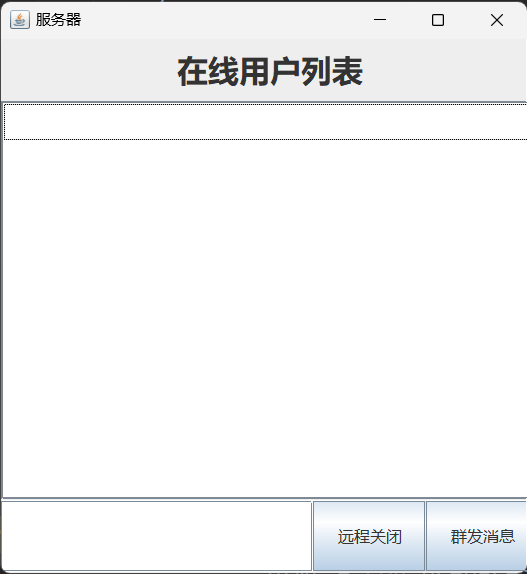
\includegraphics[width=0.4\textwidth]{img/6.png}
    \caption{服务器端运行界面}
\end{figure}

\subsection{客户端登录界面}
\begin{figure}[htbp]
    \centering
    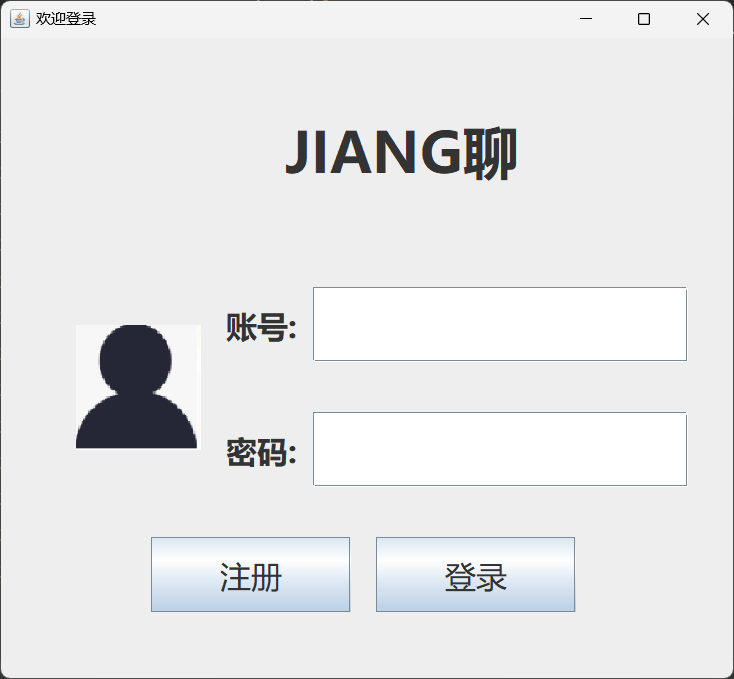
\includegraphics[width=0.4\textwidth]{img/7.png}
    \caption{客户端登录界面}
\end{figure}

\subsection{客户端注册界面}
\begin{figure}[htbp]
    \centering
    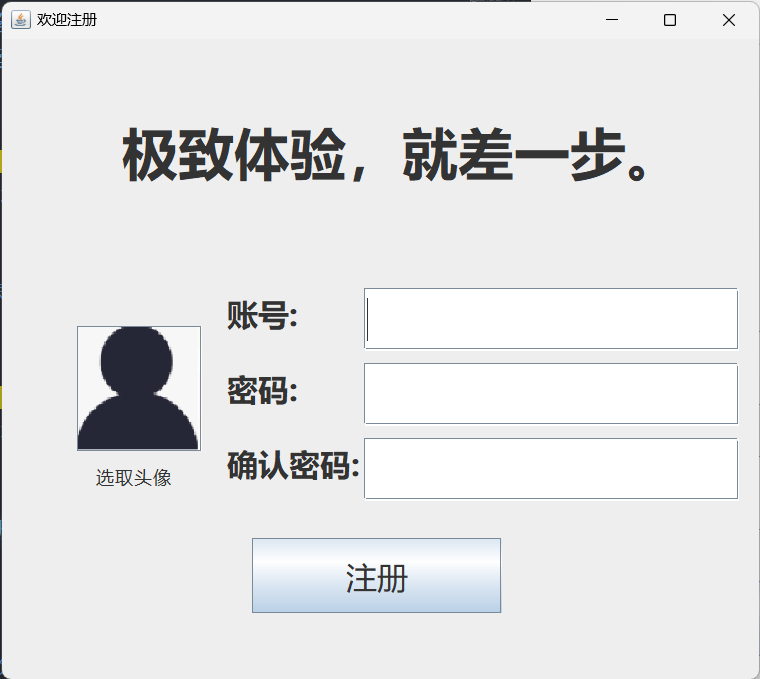
\includegraphics[width=0.4\textwidth]{img/8.png}
    \caption{客户端注册界面}
\end{figure}

\subsection{客户端注册的两种情况}
\begin{figure}[htbp]
    \centering
    \begin{minipage}{0.4\textwidth}
        \centering
        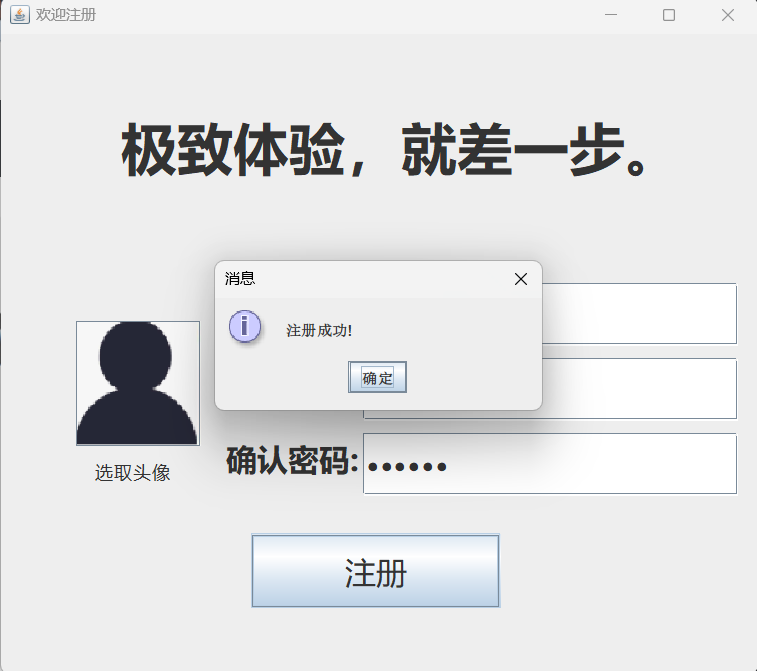
\includegraphics[width=1.0\textwidth]{img/9.png}
        \caption{客户端注册成功}
    \end{minipage}
    \begin{minipage}{0.4\textwidth}
        \centering
        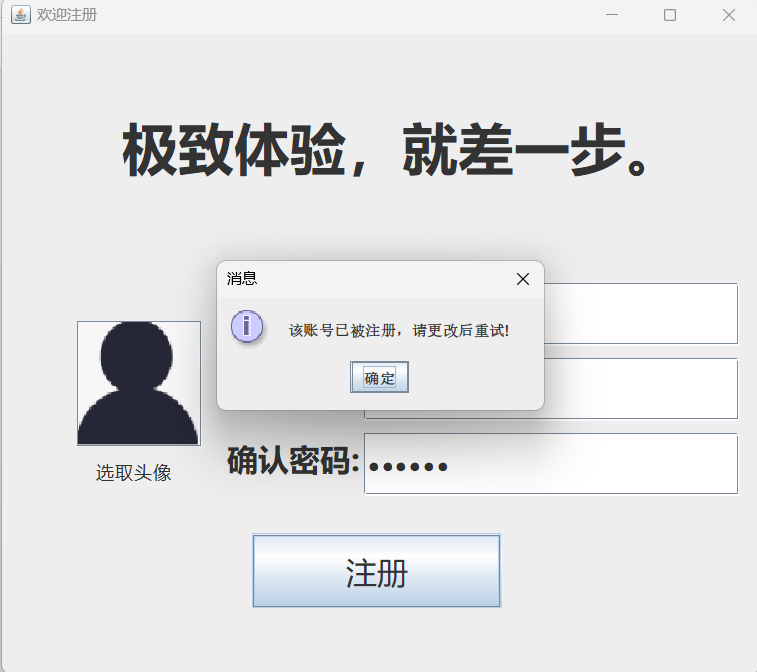
\includegraphics[width=1.0\textwidth]{img/10.png}
        \caption{客户端注册失败}
    \end{minipage}
\end{figure}

\newpage

\subsection{客户端登录的两种情况}
\begin{figure}[htbp]
    \centering
    \begin{minipage}{0.4\textwidth}
        \centering
        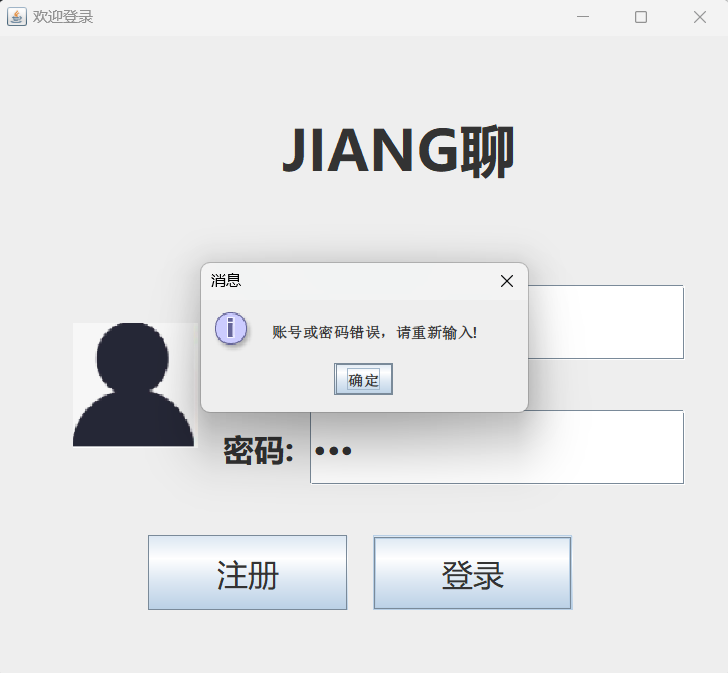
\includegraphics[width=1.0\textwidth]{img/11.png}
        \caption{客户端账号密码错误}
    \end{minipage}
    \begin{minipage}{0.4\textwidth}
        \centering
        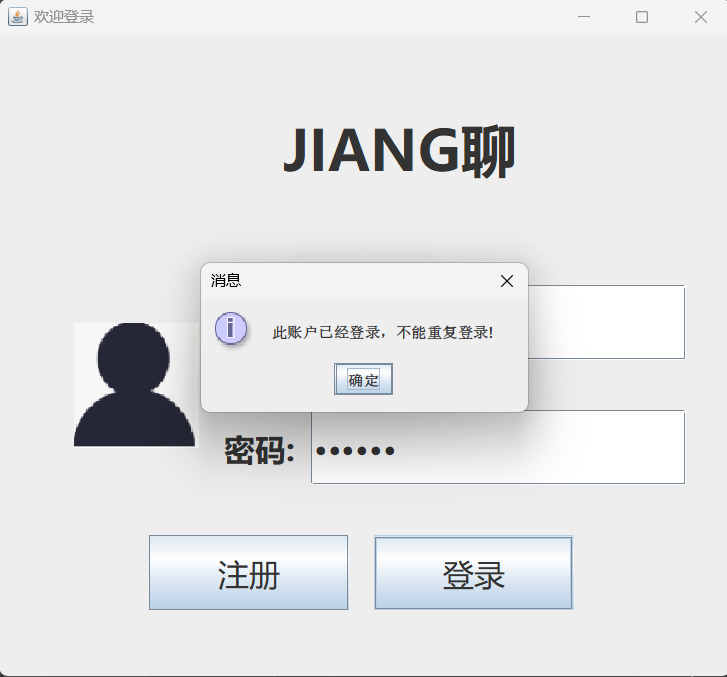
\includegraphics[width=1.0\textwidth]{img/12.png}
        \caption{客户端重复登录}
    \end{minipage}
\end{figure}

\subsection{客户端主界面}
\begin{figure}[htbp]
    \centering
    \begin{minipage}{0.4\textwidth}
        \centering
        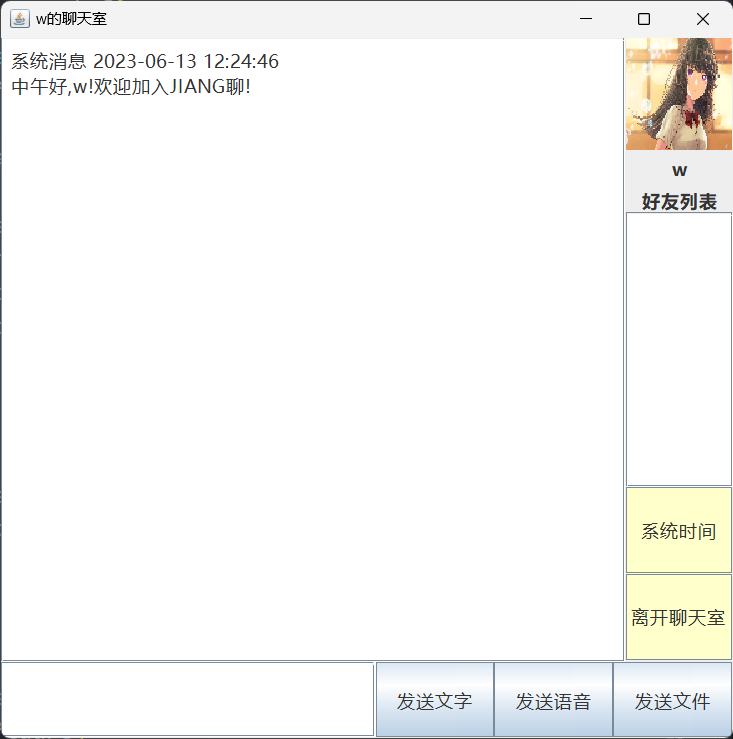
\includegraphics[width=1.0\textwidth]{img/13.png}
    \end{minipage}
    \begin{minipage}{0.4\textwidth}
        \centering
        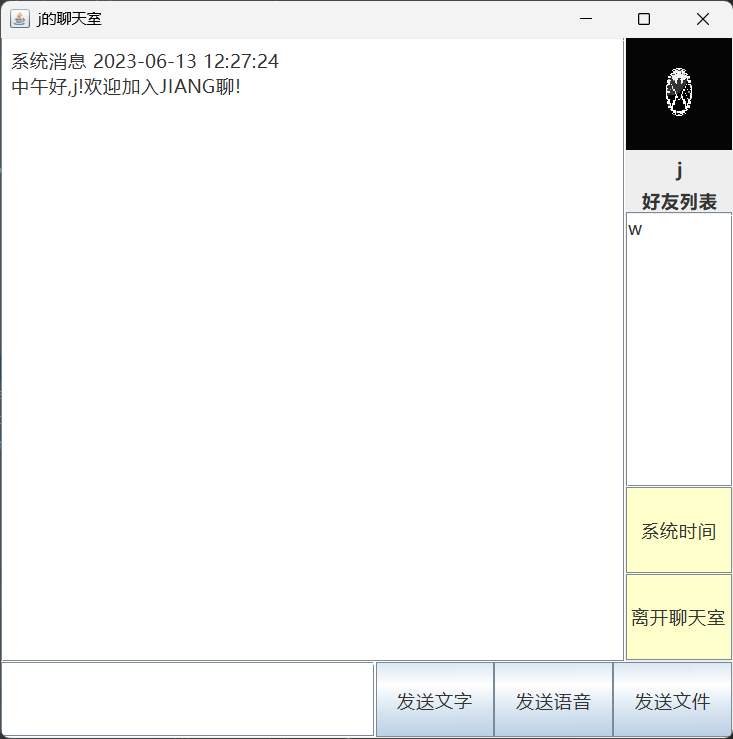
\includegraphics[width=1.0\textwidth]{img/14.png}
    \end{minipage}
    \caption{客户端主界面}
\end{figure}

\newpage

\subsection{客户端群发文字消息}
\begin{figure}[htbp]
    \centering
    \begin{minipage}{0.4\textwidth}
        \centering
        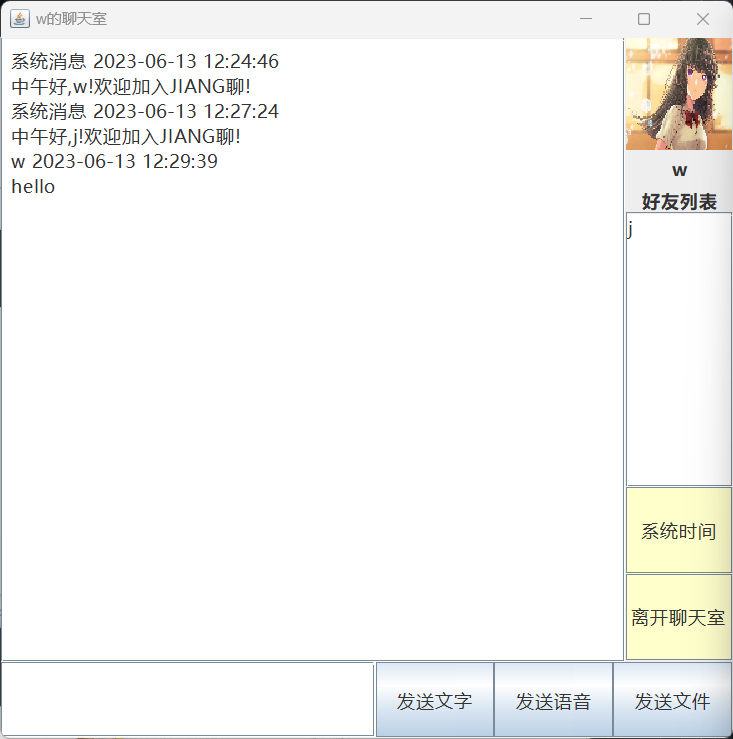
\includegraphics[width=1.0\textwidth]{img/15.png}
    \end{minipage}
    \begin{minipage}{0.4\textwidth}
        \centering
        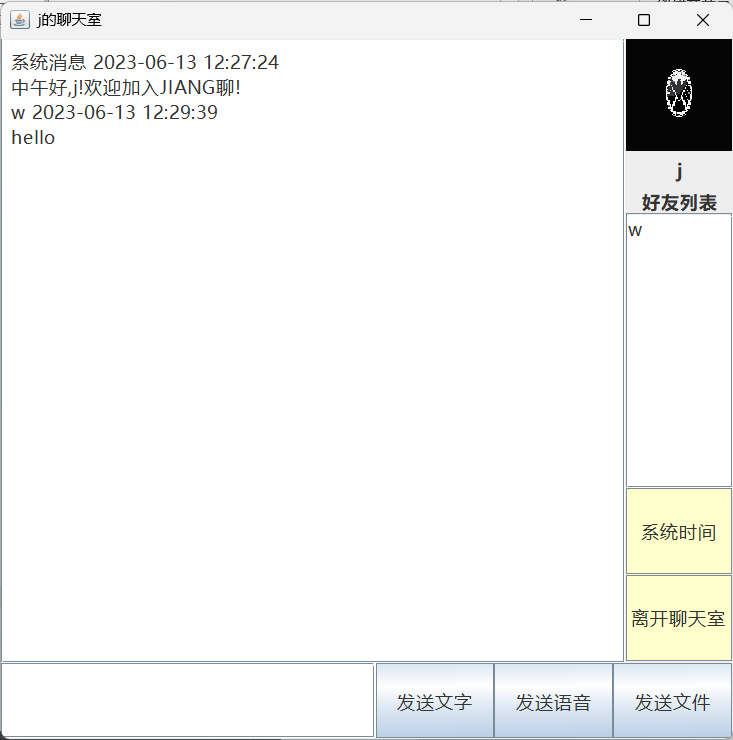
\includegraphics[width=1.0\textwidth]{img/16.png}
    \end{minipage}
    \caption{客户端群发文字消息}
\end{figure}

\subsection{客户端群发语音消息}
\begin{figure}[htbp]
    \centering
    \begin{minipage}{0.4\textwidth}
        \centering
        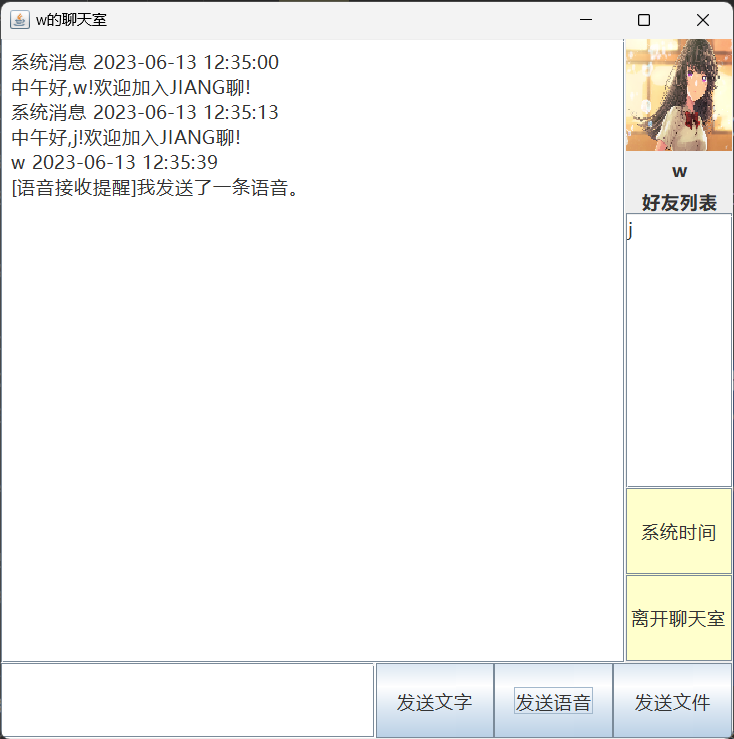
\includegraphics[width=1.0\textwidth]{img/17.png}
    \end{minipage}
    \begin{minipage}{0.4\textwidth}
        \centering
        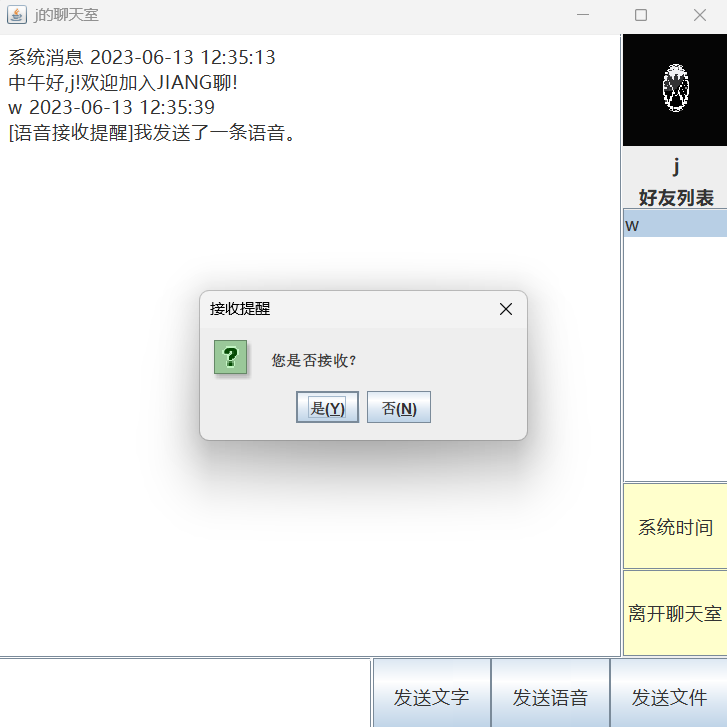
\includegraphics[width=1.0\textwidth]{img/18.png}
    \end{minipage}
    \caption{客户端群发语音消息}
\end{figure}

\newpage

\subsection{客户端群发文件}
\begin{figure}[htbp]
    \centering
    \begin{minipage}{0.4\textwidth}
        \centering
        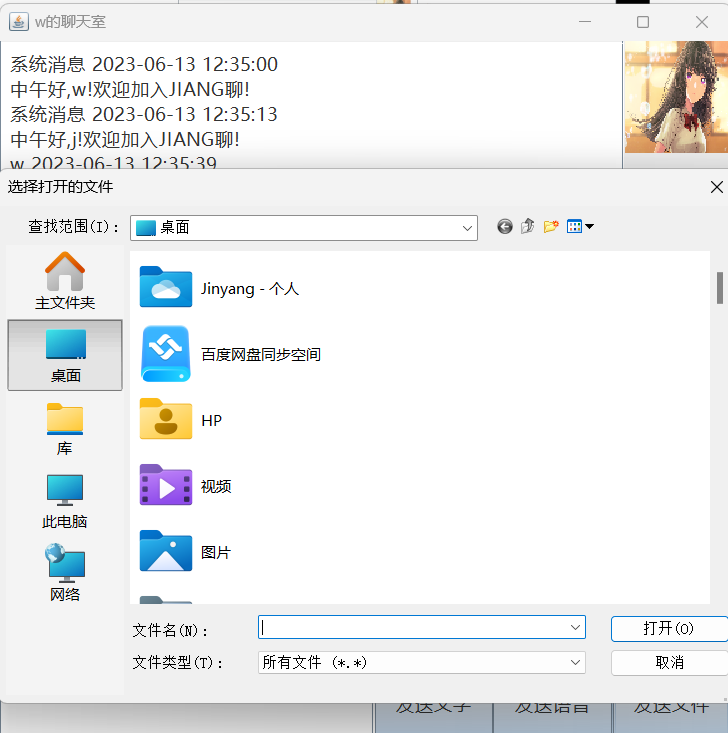
\includegraphics[width=1.0\textwidth]{img/19.png}
    \end{minipage}
    \begin{minipage}{0.4\textwidth}
        \centering
        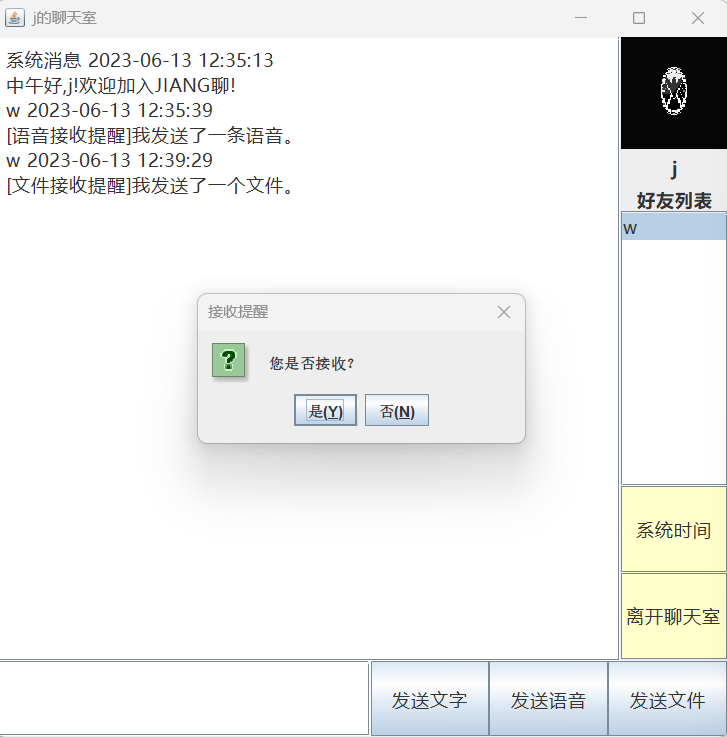
\includegraphics[width=1.0\textwidth]{img/20.png}
    \end{minipage}
    \caption{客户端群发文件}
\end{figure}

\subsection{客户端查看系统时间}
\begin{figure}[htbp]
    \centering
    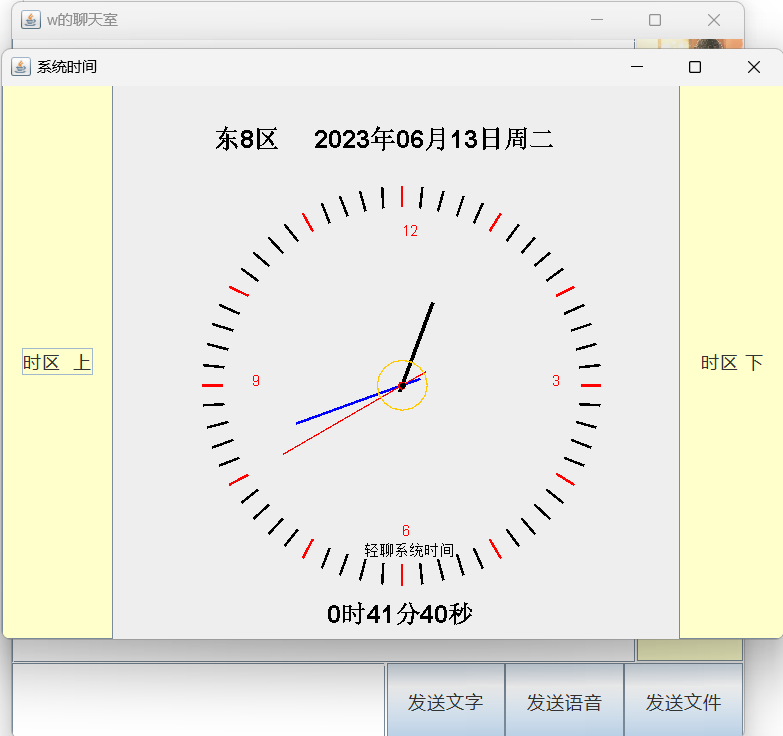
\includegraphics[width=0.5\textwidth]{img/21.png}
    \caption{客户端查看系统时间}
\end{figure}

\subsection{客户端发起私聊}
\begin{figure}[htbp]
    \centering
    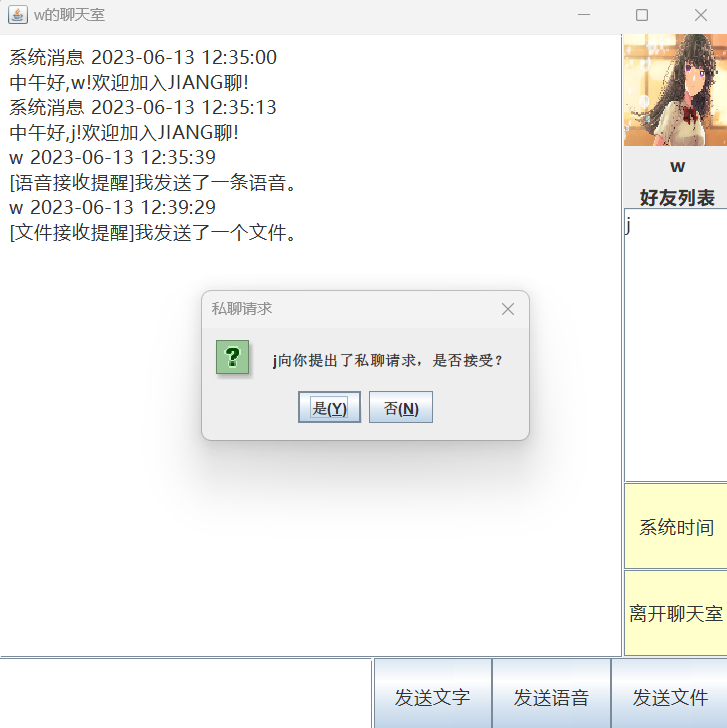
\includegraphics[width=0.4\textwidth]{img/22.png}
    \caption{客户端发起私聊}
\end{figure}

\subsection{客户端私聊}
\begin{figure}[htbp]
    \centering
    \begin{minipage}{0.4\textwidth}
        \centering
        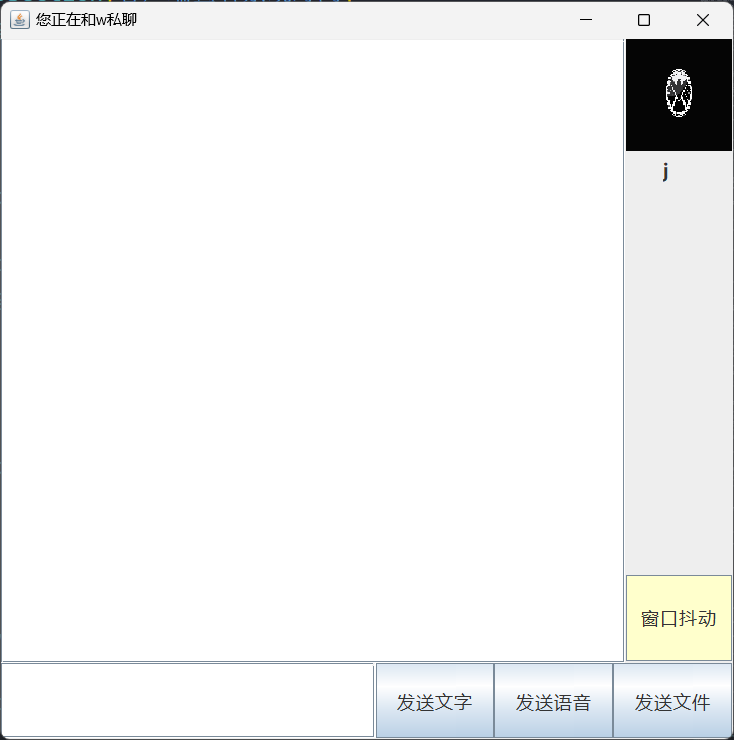
\includegraphics[width=1.0\textwidth]{img/23.png}
    \end{minipage}
    \begin{minipage}{0.4\textwidth}
        \centering
        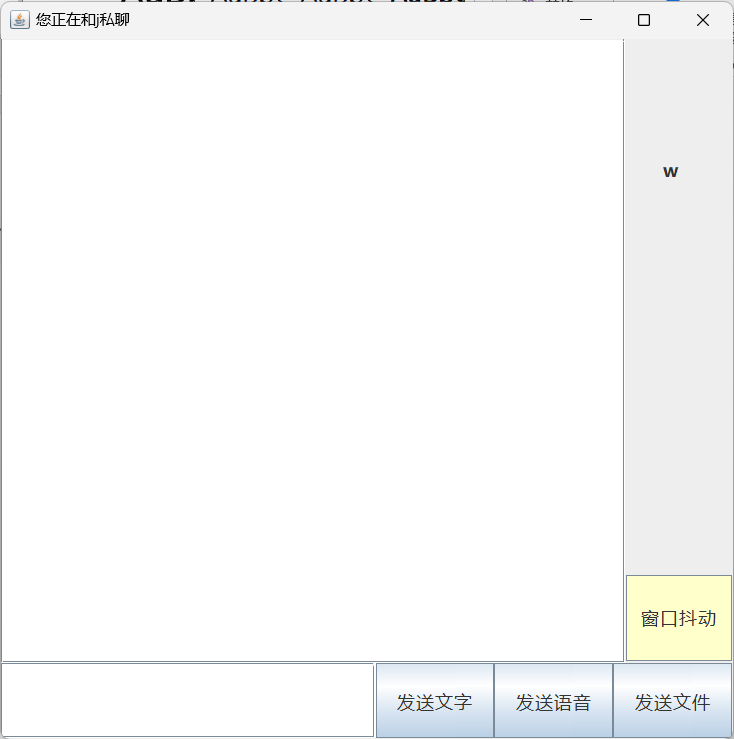
\includegraphics[width=1.0\textwidth]{img/24.png}
    \end{minipage}
    \caption{客户端私聊}
\end{figure}

\newpage

\subsection{服务器远程关闭客户端}
\begin{figure}[htbp]
    \centering
    \begin{minipage}{0.4\textwidth}
        \centering
        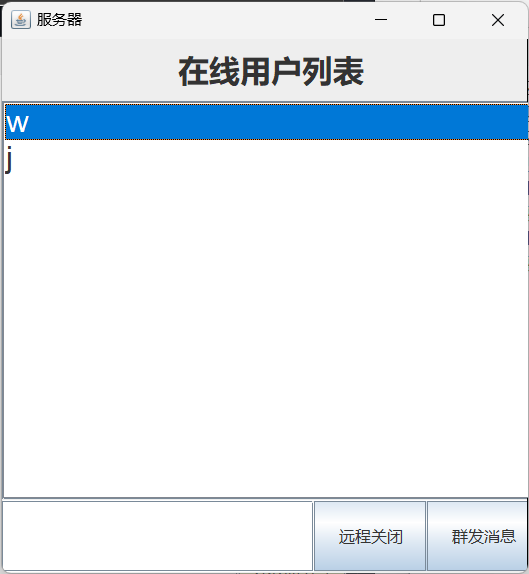
\includegraphics[width=1.0\textwidth]{img/25.png}
    \end{minipage}
    \begin{minipage}{0.4\textwidth}
        \centering
        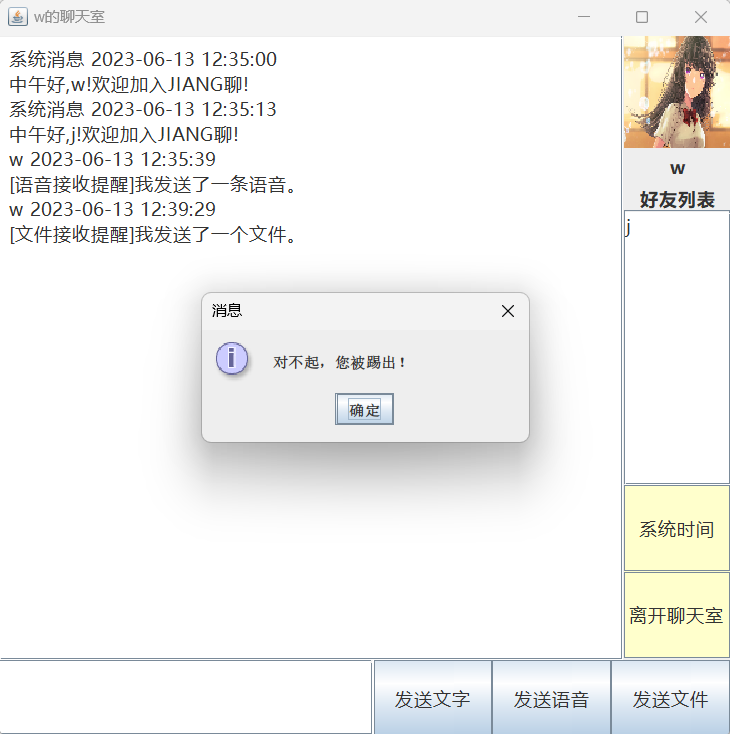
\includegraphics[width=1.0\textwidth]{img/26.png}
    \end{minipage}
    \caption{服务器远程关闭客户端}
\end{figure}

\subsection{服务器端群发系统消息}
\begin{figure}[htbp]
    \centering
    \begin{minipage}{0.4\textwidth}
        \centering
        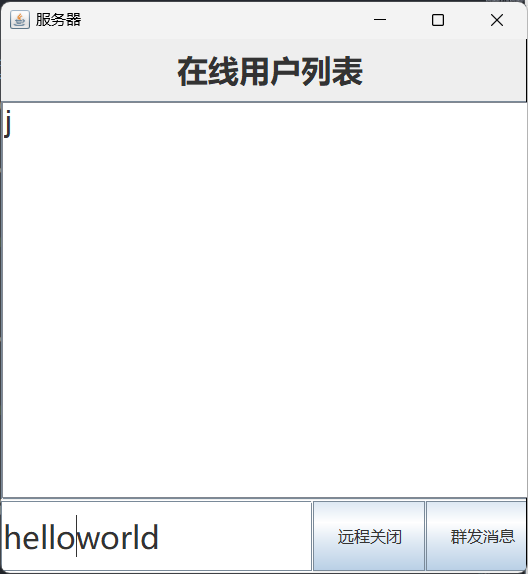
\includegraphics[width=1.0\textwidth]{img/27.png}
    \end{minipage}
    \begin{minipage}{0.4\textwidth}
        \centering
        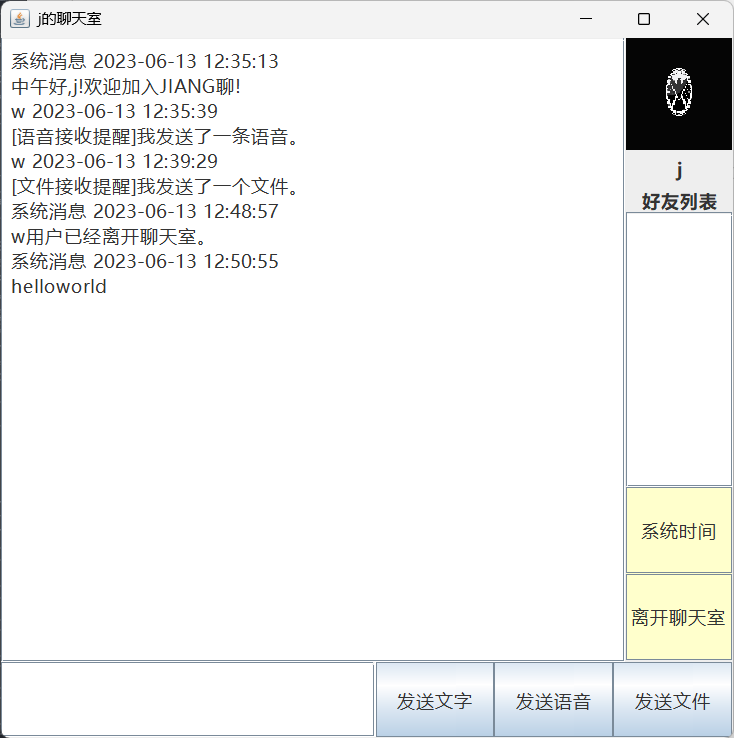
\includegraphics[width=1.0\textwidth]{img/28.png}
    \end{minipage}
    \caption{服务器端群发系统消息}
\end{figure}


\newpage

\section{白板程序业务分析}
\subsection{相关业务分析}
白板程序由教师端和学生端组成,其中为了简化逻辑,将教师端作为服务器端,学生端作为客户端,教师端和学生端之间通过socket进行通信,教师端和学生端之间的通信是双向的。
\subsubsection{教师端}
教师端启动后,进入图形化界面,包含聊天框、输入框,发送信息、发送文件、提醒听课等按钮,画图板,直线、圆形、矩形、铅笔、画笔、清空等按钮,红、黄、蓝、绿、黑、白等颜色按钮,以及在线学生的显示。

教师端可以选择自己上课需要的形状(点击相应按钮),如直线、圆形、矩形,也可以选择铅笔、画笔来进行画图;教师端相应形状颜色的绘制可以选择红色、黄色、蓝色、绿色、黑色、白色等。

当教师发现学生听课不专心时(如线下教学情况),可以点击“提醒听课”,学生端对应的学生会振动2s,并在文字显示框内显示警告信息。
\subsubsection{学生端}
当每个学生端进行连接时,会首先跳出登录界面;当用户是首次使用本系统时,可以进行注册,即点击“注册”按钮,学生端输入帐号、密码和确认密码进行注册。服务器端进行注册判定,注册完的账户当进行再次登录系统时,无需注册,直接登录即可。学生端进行登录时,首先输入帐号和密码,并点击“登录”,教师端的服务器进行登录判定,成功后开放文件传输端口并与学生端连接,同时将帐号和ChatThread类对象的对应关系记录于HashMap中,以便聊天记录的转发等,否则任意一种情况都将拒绝登录。

学生端连接课堂后,可以发送文字消息和举手发言,并同步教师端的画图板信息,显示当前在线的学生信息。

\subsection{相关业务流程图}
\subsubsection{注册、登录业务流程图}
\begin{figure}[htbp]
    \centering
    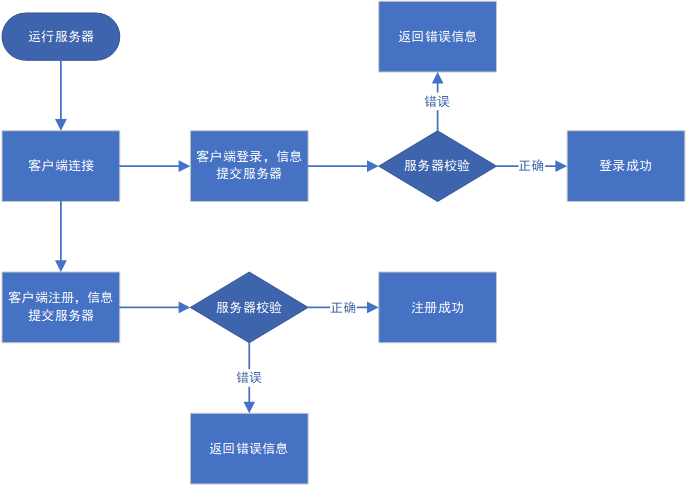
\includegraphics[width=0.7\textwidth]{img/29.png}
    \caption{注册、登录业务流程图}
\end{figure}

\subsubsection{系统业务流程图}
\begin{figure}[htbp]
    \centering
    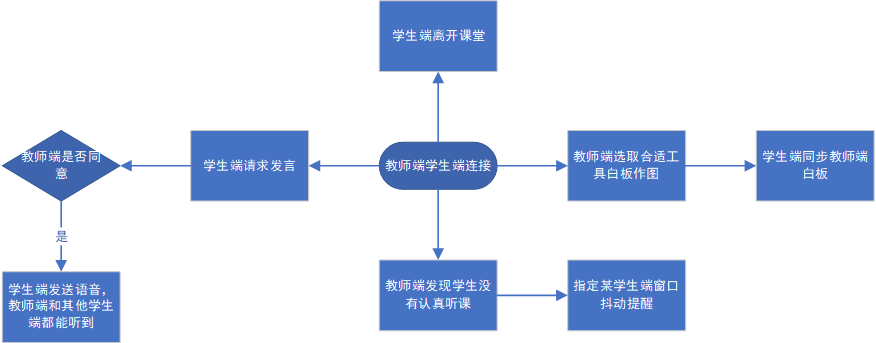
\includegraphics[width=0.7\textwidth]{img/30.png}
    \caption{系统业务流程图}
\end{figure}

\newpage

\section{白板程序系统设计}
\subsection{系统功能设计}
\begin{enumerate}
    \item java图形界面编程编写教师端(服务器端)和学生端(客户端),实现教师端和学生端的通信。实现画板的基本功能,能够实时更新画板内容。
    \item 学生端可以实现注册、登录、发送文字消息、发送文件、举手发言、同步画板、显示在线学生等功能。
    \item 教师端可以实现发送文字消息、发送文件、提醒听课、在画板上操作、显示在线学生等功能。
\end{enumerate}

\subsection{消息头部设计}
教师端和学生端之间的通信消息通过消息头部来区分,消息头部的定义非常重要。白板程序基于聊天程序改进而来,所以在消息头部的定义上,参考了聊天程序的消息头部定义,

\begin{tabular}{cc}
    \toprule
    消息头部 & 具体含义 \\
    \midrule
    REG1&检查注册时密码和确认密码一致性\\
    YES&注册密码和确认密码一致\\
    NO&注册信息有误或登录信息有误\\
    REG2&检查注册时用户名是否已经被注册\\
    EXISTS&用户名已经存在\\
    INSERT&用户名已经成功注册\\
    LOGIN&用户登录\\
    CHONG&用户重复登录,登录失败\\
    NO&用户不存在或输入信息不正确,登录失败\\
    NEW&新用户登入聊天室\\
    USER&服务器发送好友列表\\
    LOGOUT&客户端离开课堂\\
    SLOGOUT&教师端为其他客户端发送离开课堂信息\\
    LINE&教师端发送直线\\
    YUAN&教师端发送圆形\\
    JUXING&教师端发送矩形\\
    QIANBI&教师端发送铅笔\\
    HUABI&教师端发送画笔\\
    YANSE&教师端发送当前绘制颜色\\
    EMPTY&教师端发送清空画板信息\\
    RECORD&有学生举手发言\\
    OKRECORD&教师端同意学生发言\\
    NORECORD&教师端拒绝学生发言\\
    CARE&教师端提醒学生听课\\
    \bottomrule
\end{tabular}

\subsection{教师端设计}
\subsubsection{教师端的界面设计}
教师端启动后,进入图形化界面,包含聊天框、输入框,发送信息、发送文件、提醒听课等按钮,画图板,直线、圆形、矩形、铅笔、画笔、清空等功能按钮,红、黄、蓝、绿、黑、白等颜色按钮,以及在线学生的显示。

以下是界面对象的定义:
\begin{lstlisting}[title=界面对象的定义,frame=shadowbox]
    private JLabel explain = new JLabel("在线学生", JLabel.CENTER);
    private List users = new List();
    private JButton Send_Button = new JButton("发送消息");
    private JButton Send_File = new JButton("发送文件");
    private JButton Send_Remind = new JButton("提醒听课");
    private JTextField Sendword = new JTextField(20);       //发文字区域
    private JTextArea Chat = new JTextArea(10, 45);     //聊天记录显示
    private ServerSocket ss = null;
    private Font font = new Font("微软雅黑", Font.PLAIN, 14);
    private HashMap<String, ChatThread> users_connect = new HashMap<String, ChatThread>();
    private JPanel paintBoard = new JPanel();   //画图板
    private JPanel buttonBoard = new JPanel();    //按钮面板
    private JPanel jpRight = new JPanel();        //绘画面板
    private JLabel exp1 = new JLabel("智慧课堂教师端", JLabel.CENTER);
\end{lstlisting}

然后是界面的初始化,由于界面的初始化代码较多,在此处暂不列出。在界面的初始化过程中,同时绑定了端口10222,用于学生端的连接,与学生端进行通信;同时调用了数据库连接驱动,连接到数据库,在这个系统中,选择了和上一程序共享数据库,减少了开发量。

\subsubsection{教师端画板的实现}
教师端画板的实现,主要是通过鼠标事件来实现,通过鼠标事件的监听,可以实现画板的各种功能,包括直线、圆形、矩形、铅笔、画笔、清空等功能。

在画板的实现过程中,与学生端进行通信,并不直接将图像信息发送给学生端,而是将鼠标的按下XY坐标、鼠标的释放XY坐标传送给学生端,然后在学生端本地实现绘制,这样可以减少网络传输的数据量,提高了程序的健壮性。

\paragraph{鼠标按下事件侦听}
当鼠标按下时,记录鼠标的XY坐标,实现代码如下:
\begin{lstlisting}[title=鼠标按下事件侦听,frame=shadowbox]
    public void mousePressed(MouseEvent e) {
        //记录鼠标按下的坐标
        shapePoint[0] = e.getX();
        shapePoint[1] = e.getY();
    }
\end{lstlisting}

\paragraph{鼠标释放事件侦听}
当鼠标释放时,记录鼠标的XY坐标,然后对最后按下的图形按钮进行分类,依据不同的图形,分别实现不同的绘图效果。

\subparagraph{直线的绘制}
直线的绘制,只需要将传送四个坐标值,然后调用Graphics2D的drawLine方法,即可实现直线的绘制,实现代码如下:
\begin{lstlisting}[title=直线的绘制,frame=shadowbox]
    case "直线":
    //绘制直线
    g2d.drawLine(shapePoint[0], shapePoint[1], shapePoint[2], shapePoint[3]);
    //调用发送图形方法
    sendShape();
    break;
\end{lstlisting}

\subparagraph{圆形的绘制}
圆形的绘制略微复杂,先确定圆形的左上角坐标点,然后确定圆形的宽度和高度,然后调用Graphics2D的fillOval方法,绘制出来的不一定是正圆形,然后通过发送图形的统一函数进行图像的发送,实现代码如下:
\begin{lstlisting}[title=圆形的绘制,frame=shadowbox]
    case "圆形":
    //记录圆形左上角坐标点,并计算其宽高
    int x1 = Math.min(shapePoint[0], shapePoint[2]);
    int y1 = Math.min(shapePoint[1], shapePoint[3]);
    int width = Math.abs(shapePoint[0] - shapePoint[2]);
    int height = Math.abs(shapePoint[1] - shapePoint[3]);
    shapePoint[0] = x1;
    shapePoint[1] = y1;
    shapePoint[2] = width;
    shapePoint[3] = height;
    //绘制椭圆
    g2d.fillOval(shapePoint[0], shapePoint[1], shapePoint[2], shapePoint[3]);
    //调用发送图形方法
    sendShape();
    break;
\end{lstlisting}

\subparagraph{矩形的绘制}
矩形的绘制与圆形的绘制类似,先确定矩形的左上角坐标点,然后确定矩形的宽度和高度,然后调用Graphics2D的fillRect方法,绘制出来的不一定是正矩形,然后通过发送图形的统一函数进行图像的发送,实现代码如下:
\begin{lstlisting}[title=矩形的绘制,frame=shadowbox]
    case "矩形":
    x1 = Math.min(shapePoint[0], shapePoint[2]);
    y1 = Math.min(shapePoint[1], shapePoint[3]);
    width = Math.abs(shapePoint[0] - shapePoint[2]);
    height = Math.abs(shapePoint[1] - shapePoint[3]);
    shapePoint[0] = x1;
    shapePoint[1] = y1;
    shapePoint[2] = width;
    shapePoint[3] = height;
    g2d.fillRect(shapePoint[0], shapePoint[1], shapePoint[2], shapePoint[3]);
    sendShape();
    break;
\end{lstlisting}

\subparagraph{铅笔、画笔的绘制}
铅笔、画笔在画板上直接进行绘制,因此需要重写鼠标拖动事件,实现代码如下:
\begin{lstlisting}[title=铅笔、画笔的绘制,frame=shadowbox]
    public void mouseDragged(MouseEvent e) {
        if (nowButton.equals("铅笔") || nowButton.equals("画笔")) {
            shapePoint[2] = shapePoint[0];
            shapePoint[3] = shapePoint[1];

            shapePoint[0] = e.getX();
            shapePoint[1] = e.getY();

            g2d.drawLine(shapePoint[0], shapePoint[1], shapePoint[2], shapePoint[3]);

            sendShape();
        }
    }
\end{lstlisting}

接下来,将对统一的发送图形函数进行定义,实现代码如下:
\begin{lstlisting}[title=统一的发送图形函数,frame=shadowbox]
    public void sendShape() {
        try {
            switch (nowButton) {
                case "直线":
                    for (String ct : users_connect.keySet()) {    //利用key值遍历哈希表
                        users_connect.get(ct).Send.println("LINE-" + shapePoint[0]
                                + "-" + shapePoint[1] + "-" + shapePoint[2] + "-" + shapePoint[3]);
                    }
                    break;
                case "圆形":
                    for (String ct : users_connect.keySet()) {    //利用key值遍历哈希表
                        users_connect.get(ct).Send.println("YUAN-" + shapePoint[0]
                                + "-" + shapePoint[1] + "-" + shapePoint[2] + "-" + shapePoint[3]);
                    }
                    break;
                case "矩形":
                    for (String ct : users_connect.keySet()) {    //利用key值遍历哈希表
                        users_connect.get(ct).Send.println("JUXING-" + shapePoint[0]
                                + "-" + shapePoint[1] + "-" + shapePoint[2] + "-" + shapePoint[3]);
                    }
                    break;
                case "铅笔":
                    for (String ct : users_connect.keySet()) {    //利用key值遍历哈希表
                        users_connect.get(ct).Send.println("QIANBI-" + shapePoint[0]
                                + "-" + shapePoint[1] + "-" + shapePoint[2] + "-" + shapePoint[3]);
                    }
                    break;
                case "画笔":
                    for (String ct : users_connect.keySet()) {    //利用key值遍历哈希表
                        users_connect.get(ct).Send.println("HUABI-" + shapePoint[0]
                                + "-" + shapePoint[1] + "-" + shapePoint[2] + "-" + shapePoint[3]);
                    }
            }
        } catch (Exception e) {
        }
    }
\end{lstlisting}

此外,还需要对绘制图像的颜色进行发送,实现方法是遍历在线客户端哈希表,然后使用消息头部“YANSE-”+Color,实现代码如下:
\begin{lstlisting}[title=绘制图像的颜色进行发送,frame=shadowbox]
    public void sendColor(String Color) {
        try {
            for (String ct : users_connect.keySet()) {    //利用key值遍历哈希表
                users_connect.get(ct).Send.println("YANSE-" + Color);     //发送颜色的单词
            }
        } catch (Exception e) {
        }
    }
\end{lstlisting}

\subparagraph{清空画板}
系统还提供了清空画板的功能,点击清空按钮,服务器端将清空消息发送给所有的客户端,在其本地实现画板的清空,同时服务器端也清空画板,实现代码如下:
\begin{lstlisting}[title=清空画板,frame=shadowbox]
    public void sendEmpty() {
        try {
            for (String ct : users_connect.keySet()) {    //利用key值遍历哈希表
                users_connect.get(ct).Send.println("EMPTY");    //发送清空信号
            }
        } catch (Exception e) {
        }
    }
\end{lstlisting}

\subsubsection{教师端活动监听器的实现}
教师端的活动监听器主要是对按钮的监听,包括发送消息、发送文件、提醒听课、直线、圆形、矩形、铅笔、画笔、清空等按钮的监听。

\paragraph{发送消息按钮的监听}
点击发送消息按钮后,获取消息输入框中的内容,在服务器端进行消息的整合,将加上消息头部的消息发送给所有的客户端,同时在聊天框中显示发送的消息,全部完成后清空输入框:

\begin{lstlisting}[title=发送消息按钮的监听,frame=shadowbox]
    if (e.getSource() == Sendword || e.getSource() == Send_Button) {
        //群发消息按钮
        for (String ct : users_connect.keySet()) {    //利用key值遍历哈希表
            users_connect.get(ct).Send.println("教师 " + new SimpleDateFormat("yyyy-MM-dd HH:mm:ss").format(new Date()));
            users_connect.get(ct).Send.println(Sendword.getText());
        }
        String sim = new SimpleDateFormat("yyyy-MM-dd HH:mm:ss").format(new Date());
        Chat.append("教师 " + sim + "\n");
        Chat.append(Sendword.getText() + "\n");
        Sendword.setText("");       //清空输入框
    }
\end{lstlisting}

\paragraph{发送文件按钮的监听}
点击发送文件按钮后,弹出文件选择框,选择文件后,将文件名和文件长度发送给所有的客户端,然后将文件内容发送给所有的客户端,实现代码如下:

\begin{lstlisting}[title=发送文件按钮的监听,frame=shadowbox]
    else if (e.getSource() == Send_File) {
        FileDialog fLoader = new FileDialog(this, "选择打开的文件", FileDialog.LOAD);
        fLoader.setVisible(true);
        String path = fLoader.getDirectory() + fLoader.getFile();
        FileReadAndWrite.outFileToClient(path);    //将文件分发给学生端
        //群发消息按钮
        for (String ct : users_connect.keySet()) {    //利用key值遍历哈希表
            users_connect.get(ct).Send.println("教师 " + new SimpleDateFormat("yyyy-MM-dd HH:mm:ss").format(new Date()));
            users_connect.get(ct).Send.println("[文件接收提醒]我发送了一个文件。");
        }
        String sim = new SimpleDateFormat("yyyy-MM-dd HH:mm:ss").format(new Date());
        Chat.append("教师 " + sim + "\n");
        Chat.append("[文件接收提醒]我发送了一个文件。\n");
    }
\end{lstlisting}

\paragraph{提醒听课按钮的监听}
在提醒学生注意听课之前,先需要选中一个学生,然后点击提醒听课按钮,服务器端将提醒消息发送给选中的学生,学生端处理消息,并产生窗口抖动的效果,同时在消息框内追加提示信息,实现代码如下:

\begin{lstlisting}[title=提醒听课按钮的监听,frame=shadowbox]
    else if (e.getSource() == Send_Remind) {
        //提醒认真听课
        String selectedUser = users.getSelectedItem();
        String msg = "CARE";
        ChatThread ct = users_connect.get(selectedUser);
        ct.Send.println(msg);       //CARE提醒
        String sim = new SimpleDateFormat("yyyy-MM-dd HH:mm:ss").format(new Date());
        ct.Send.println("教师 " + sim);
        ct.Send.println("[警告]请务必集中注意力,认真听讲!");
        Chat.append("教师 " + sim + "\n");
        Chat.append("[警告]请务必集中注意力,认真听讲!\n");
    }
\end{lstlisting}

\paragraph{直线、圆形、矩形、铅笔、画笔、清空等按钮的监听}
在上面所解释的所有按钮都没有被按下,同时监听到有活动,那么就是直线、圆形、矩形、铅笔、画笔、清空等按钮被按下,此时,需要将按钮的名称记录下来,然后在鼠标释放事件中进行判断,实现代码如下:

\begin{lstlisting}[title=直线、圆形、矩形、铅笔、画笔、清空等按钮的监听,frame=shadowbox]
    else {          //为绘图部分的按钮
    String name = e.getActionCommand();       //先获取触发事件命令名称
    switch (name) {
        case "直线", "圆形", "矩形", "铅笔" -> {
            g2d.setStroke(new BasicStroke(3.0f));
            nowButton = name;
        }     //将当前的button设为命令名字
        case "画笔" -> {
            g2d.setStroke(new BasicStroke(5.0f));   //设置画笔宽度
            nowButton = name;
        }
        case "清空" -> {
            paintBoard.paint(g2d);
            sendEmpty();
        }
        case "红" -> {
            g2d.setColor(Color.red);
            Now_color = "RED";
            sendColor("RED");
        }
        case "黄" -> {
            g2d.setColor(Color.yellow);
            Now_color = "YELLOW";
            sendColor("YELLOW");
        }
        case "蓝" -> {
            g2d.setColor(Color.blue);
            Now_color = "BLUE";
            sendColor("BLUE");
        }
        case "绿" -> {
            g2d.setColor(Color.green);
            Now_color = "GREEN";
            sendColor("GREEN");
        }
        case "黑" -> {
            g2d.setColor(Color.black);
            Now_color = "BLACK";
            sendColor("BLACK");
        }
        case "白" -> {
            g2d.setColor(Color.white);
            Now_color = "WHITE";
            sendColor("WHITE");
        }
    }
}
\end{lstlisting}

至此,教师端的所有功能都已经实现。

\subsection{学生端设计}
学生端的功能主要有三个窗体:登录窗体、注册窗体、上课窗体。由于登录窗体和注册窗体和上述聊天程序的登录窗体和注册窗体相同,因此直接在聊天程序的基础上进行微调,主要需要修改的是上课窗体。

\subsubsection{学生端界面设计}
学生端启动后,进入图形化界面,包含聊天框、输入框,发送信息、发送文件、举手发言等按钮,画图板,直线、圆形、矩形、铅笔、画笔、清空等功能按钮,红、黄、蓝、绿、黑、白等颜色按钮,以及在线学生的显示。

以下是界面对象的定义:
\begin{lstlisting}[title=界面对象的定义,frame=shadowbox]
    private JScrollPane jsp = new JScrollPane();
    private JButton Send = new JButton("发送消息");
    private JButton Send_Record = new JButton("举手发言");
    private JButton Leave = new JButton("离开课堂");
    private DefaultListModel<String> user = new DefaultListModel<String>();  //用户列表
    private JList<String> userList = new JList<String>(user);   //展示用户列表
    private JScrollPane listPane = new JScrollPane(userList);       //设置滚动视图
    private JTextField Sendword = new JTextField(20);       //发文字区域
    private JTextArea Chat = new JTextArea(10,45);     //聊天记录显示
    private JLabel myself = new JLabel("",JLabel.CENTER);
    private JLabel friend_list = new JLabel("在线学生",JLabel.CENTER);
    private JLabel exp1 = new JLabel("智慧课堂学生端",JLabel.CENTER);
    private JPanel paintBoard = new JPanel();   //画图板
\end{lstlisting}

然后是界面的初始化,由于界面的初始化代码较多,在此处暂不列出。在界面的初始化过程中,同时绑定了端口10222,用于教师端的连接,与教师端进行通信。在初始化中,值得一提的是学生端的头像,头像是通过数据库进行存储的,因此需要从数据库中读取头像,然后显示在界面上,实现代码如下:

\begin{lstlisting}[title=学生端的头像,frame=shadowbox]
    ImageIcon image = new ImageIcon(path);  //将图片路径作为参数传入
    image.setImage(image.getImage().getScaledInstance(85,90,Image.SCALE_DEFAULT));  //创建缩放版本图像
    JLabel Picture = new JLabel(image);
    Picture.setLocation(1100,0);
    Picture.setSize(85,90);
\end{lstlisting}

\subsubsection{学生端run方法的实现}
在学生端run方法中,主要是对消息头部的判断,然后进行相应的处理,包括接收消息、接收文件、接收图像、接收图形、接收颜色、接收清空等。首先从输入流中读取消息,然后依据“-”进行split,实现代码如下:

\begin{lstlisting}
    String message = br.readLine();
    String[] msgs = message.split("-");
\end{lstlisting}

然后根据划分出来的第一个元素即消息头部进行判定,执行相应的操作。

\paragraph{退出课堂}
退出课堂的消息头部是“LOGOUT”,当学生端收到“LOGOUT”消息头部时,首先向服务器发送“RUN”消息使服务器能够广播该学生端的离开课堂信息,然后弹窗提醒学生已成功下线,最后关闭学生端的窗口,实现代码如下:

\begin{lstlisting}[title=退出课堂,frame=shadowbox]
    if(msgs[0].equals("LOGOUT")){//退出课堂
    ps.println("RUN-"+NickName);        //使服务器能够让别人知道消息
    JOptionPane.showMessageDialog(this, "您已离开课堂!再见!");
    this.dispose();
    }
\end{lstlisting}

\paragraph{有人进入课堂}
接收到消息头部为“SLOGIN”时,学生客户端的聊天框追加欢迎信息,同时将新用户的用户名添加到用户列表中,实现代码如下:

\begin{lstlisting}[title=有人进入课堂,frame=shadowbox]
    else if(msgs[0].equals("SLOGIN")){//有人进入课堂
    Chat.append("欢迎"+msgs[1]+"进入课堂!\n");
    if(!msgs[1].equals(NickName)){
        user.addElement(msgs[1]);       //将用户加入好友列表
    }
    userList.repaint();
}
\end{lstlisting}

\paragraph{有人离开课堂}
接收到消息头部为“SLOGOUT”时,将离开用户的用户名从用户列表中删除,实现代码如下:

\begin{lstlisting}[title=有人离开课堂,frame=shadowbox]
    else if(msgs[0].equals("SLOGOUT")){//有人离开课堂
    user.removeElement(msgs[1]);    //将用户移除好友列表
    userList.repaint();
}
\end{lstlisting}

\paragraph{提醒听课}
接收到消息头部为“CARE”时,抖动窗口提醒学生注意听课,同时在聊天框中追加提醒信息。抖动依靠独立的线程,通过在短时间内快速改变窗体的坐标实现,实现代码如下:

\begin{lstlisting}[title=提醒听课,frame=shadowbox]
    else if(msgs[0].equals("CARE")){//提醒专心听课
    JFrame jf = this;				//获得现在的界面
    new Thread() {      //开启窗口抖动线程
        long begin = System.currentTimeMillis();
        long end = System.currentTimeMillis();
        Point p = jf.getLocationOnScreen();
        public void run() {//实现窗口抖动
            int i = 1;
            while ((end - begin) / 1000 < 2) {
                jf.setLocation(new Point((int) p.getX() - 5 * i, (int) p.getY() + 5 * i));  //Point函数构造并初始化点
                end = System.currentTimeMillis();
                try {
                    Thread.sleep(5);
                    i = -i;
                    jf.setLocation(p);
                } catch (InterruptedException e) {
                    e.printStackTrace();
                }
            }
        }
    }.start();
}
\end{lstlisting}

\paragraph{教师同意或拒绝学生发言}
接收到消息头部“OKRECORD”时,同意发言请求,弹出录制界面,创建录制线程,开始录制,实现代码如下:

\begin{lstlisting}[title=教师同意或拒绝学生发言,frame=shadowbox]
    else if(msgs[0].equals("OKRECORD")){//教师同意发言请求
    re = new RecordMain();           //进入录制界面
    re.setLocationRelativeTo(this);  //设置在本页面中间
    WaitingThread waiting = new WaitingThread();
    waiting.start();
}
\end{lstlisting}

其中,创建了一个waiting线程,用于等待录制线程结束,每隔50ms检查一次录制线程是否结束,如果结束,则关闭录制界面,通过ClientFileThread线程将录制的文件发送给教师端,实现代码如下:

\begin{lstlisting}[title=等待录制线程结束,frame=shadowbox]
    class WaitingThread extends Thread{
        public void run(){
            while(true){
                try{
                    Thread.sleep(50);//每隔50毫秒检查一次
                }catch(Exception e){}
                if(RecordMain.flag){
                    //已经录完,利用该函数发送文件到服务器
                    ClientFileThread.outFileToServer(MyRecorder.path);
                    RecordMain.flag = false;    //将值设为false,用于下一次发语音
                    break;
                }
            }
        }
    }
\end{lstlisting}

如果教师拒绝学生发言,则在学生端直接弹窗告知学生,实现代码如下:
\begin{lstlisting}
    else if(msgs[0].equals("NORECORD")){//教师拒绝发言请求
        JOptionPane.showMessageDialog(this,"教师拒绝了您的发言请求!");
    }
\end{lstlisting}

\paragraph{画板部分的修改操作}
学生端部分画板的修改操作主要是绘制图形的修改、绘制颜色修改和画布的清空操作。

\subparagraph{绘制图形的修改}
在条件判断时,将所有与图形有关的都判定进来,因此还需要进一步判定。在画板中,如果是直线绘制、铅笔绘制则设置画笔粗细为3.0f,如果是画笔绘制则设置画笔粗细为5.0f。最后调用readShape函数,根据绘制的图形以及四个XY坐标进行相应图形的绘制,实现代码如下:

\begin{lstlisting}[title=绘制图形的修改,frame=shadowbox]
    else if(msgs[0].equals("LINE") ||msgs[0].equals("YUAN")||
    msgs[0].equals("JUXING")||msgs[0].equals("QIANBI")||msgs[0].equals("HUABI")) {
//改变画笔的粗细
if(msgs[0].equals("LINE")){
    g2d.setStroke(new BasicStroke(3.0f));
}
if(msgs[0].equals("QIANBI")){
    g2d.setStroke(new BasicStroke(3.0f));
}else if(msgs[0].equals("HUABI")){
    g2d.setStroke(new BasicStroke(5.0f));
}
//动作类型+四个点
readShape(msgs[0],Integer.parseInt(msgs[1]),Integer.parseInt(msgs[2]),
        Integer.parseInt(msgs[3]),Integer.parseInt(msgs[4]));
}
\end{lstlisting}

其中readShape函数通过简单的switch-case函数进行判断,然后调用Graphics2D的相应方法进行绘制,实现代码如下:

\begin{lstlisting}[title=readShape函数,frame=shadowbox]
    public void readShape(String OP,int point1,int point2,int point3,int point4){
        //只要是传输两个点的图形绘制操作都可以用这一条
        try {
            switch(OP){
                case "LINE":
                case "QIANBI":
                case "HUABI":
                    g2d.drawLine(point1,point2,point3,point4);break;//画线
                case "YUAN":
                    g2d.fillOval(point1,point2,point3,point4);break;//画圆
                case "JUXING":
                    g2d.fillRect(point1,point2,point3,point4);break;//画矩形
            }
        } catch (Exception e) {}
    }
\end{lstlisting}

绘制颜色的修改依赖changeColor函数,根据消息头部的颜色名称,进行相应的颜色修改,实现代码如下:

\begin{lstlisting}[title=绘制颜色的修改,frame=shadowbox]
    else if(msgs[0].equals("YANSE")){//改变画笔颜色
        changeColor(msgs[1]);
    }
\end{lstlisting}

其中,changeColor函数通过简单的switch-case函数进行判断,然后调用Graphics2D的setColor方法进行颜色的修改,实现代码如下:

\begin{lstlisting}[title=changeColor函数,frame=shadowbox]
    public void changeColor(String color){//改变画笔颜色
        try {
            switch(color){
                case "RED": g2d.setColor(Color.red);break;
                case "YELLOW":
                    g2d.setColor(Color.yellow);break;
                case "BLUE": g2d.setColor(Color.blue);break;
                case "GREEN":g2d.setColor(Color.green); break;
                case "BLACK":g2d.setColor(Color.black); break;
                case "WHITE":g2d.setColor(Color.white); break;
            }
        } catch (Exception e) {}
    }
\end{lstlisting}

画布的清空操作依赖paint函数,调用paint函数进行画布的清空,实现代码如下:

\begin{lstlisting}[title=画布的清空操作,frame=shadowbox]
    else if(msgs[0].equals("EMPTY")){
        paintBoard.paint(g2d);			//画布清空
    }
\end{lstlisting}

\subsubsection{学生端活动监听器的实现}
学生端的活动监听器主要是对按钮的监听,包括发送消息、发送文件、举手发言、直线、圆形、矩形、铅笔、画笔、清空等按钮的监听,实现代码如下:

\begin{lstlisting}[title=学生端活动监听器的实现,frame=shadowbox]
    public void actionPerformed(ActionEvent e){
        if(e.getSource() == Send || e.getSource() == Sendword) {//发送消息
            ps.println(NickName + "-" + Sendword.getText());
            Sendword.setText("");               //清空文本框
        }
        else if(e.getSource() == Send_Record){//举手发言
            ps.println("RECORD-"+NickName);
        }else if(e.getSource() == Leave){      //要走了
            ps.println("LEAVE");
        }
    }
\end{lstlisting}

还有学生端的私聊功能的实现,还需要对用户列表、鼠标的双击事件进行监听,实现代码如下:

\begin{lstlisting}[title=鼠标双击事件的监听,frame=shadowbox]
    public void mouseClicked(MouseEvent e) {
        if(e.getClickCount() == 2) {        //监听双击事件
            ps.println("SILIAO" + "-" + userList.getSelectedValue());       //向服务器发送想私聊信息
        }
    }
\end{lstlisting}

至此,学生端的主要功能已经实现。

\subsection{双端文件传输线程的实现}
本实验中,将文件传输线程设计为一个独立的线程用于接收文件,文件传输线程承担了传输普通文件和语音文件的任务,使用独立端口,使得通信和传输分离,提高了程序的健壮性。

在本程序中,文件传输线程依旧在两端分别实现,两者的实现方式与聊天室的程序相似,因此不再赘述。

\newpage

\section{白板程序源代码清单}
\subsection{Package Student}
\paragraph{ClientFileThread.java}
\paragraph{Login.java}
\paragraph{MyRecorder.java}
\paragraph{RecordMain.java}
\paragraph{Register.java}
\paragraph{Student.java}

\subsection{Package Teacher}
\paragraph{ServerFileThread.java}
\paragraph{Teacher.java}

\newpage

\section{白板程序运行结果与测试分析}
\subsection{教师端运行结果}
\begin{figure}[htbp]
    \centering
    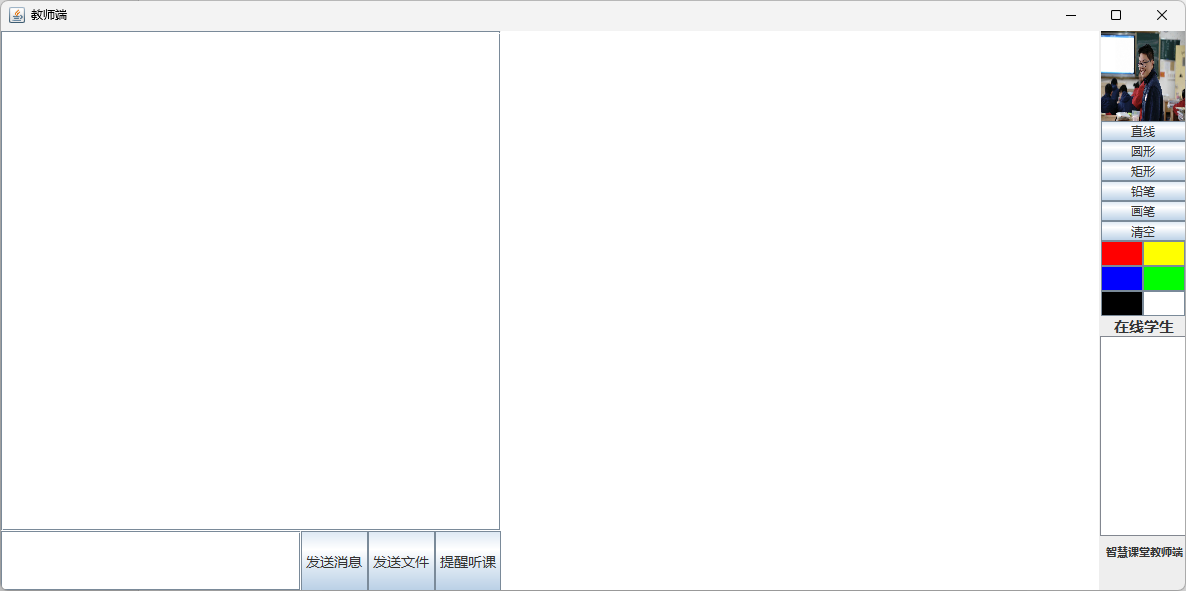
\includegraphics[width=0.8\textwidth]{img/31.png}
    \caption{教师端登录}
\end{figure}

\subsection{学生端运行结果}
\begin{figure}[htbp]
    \centering
    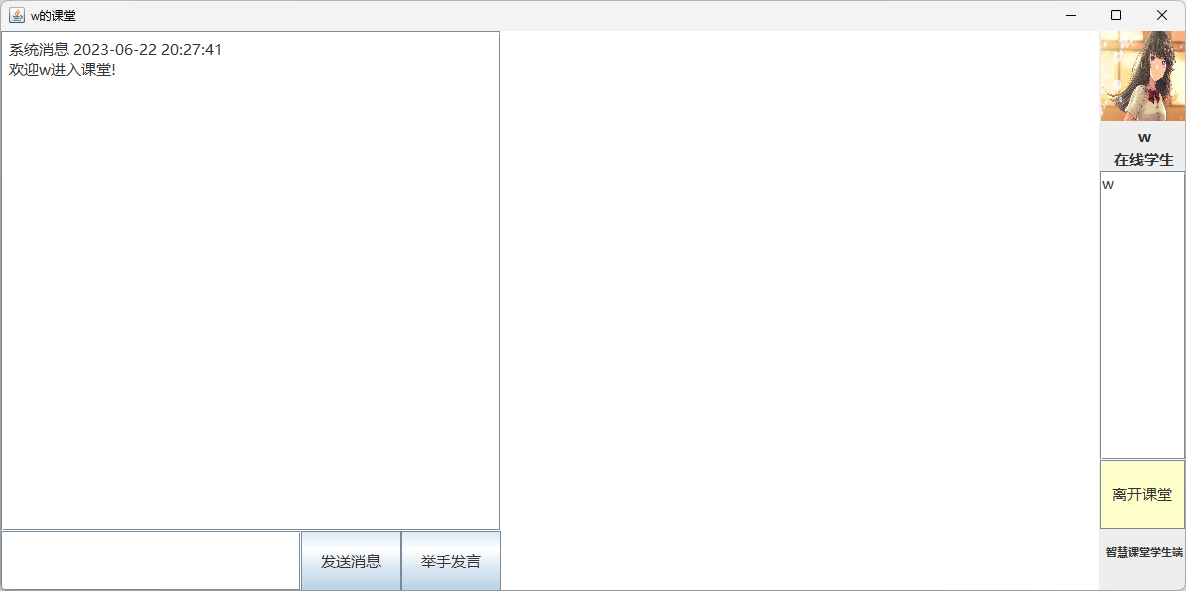
\includegraphics[width=0.8\textwidth]{img/32.png}
    \caption{学生端登录}
\end{figure}

\subsection{画板绘图结果}
\begin{figure}[htbp]
    \centering
    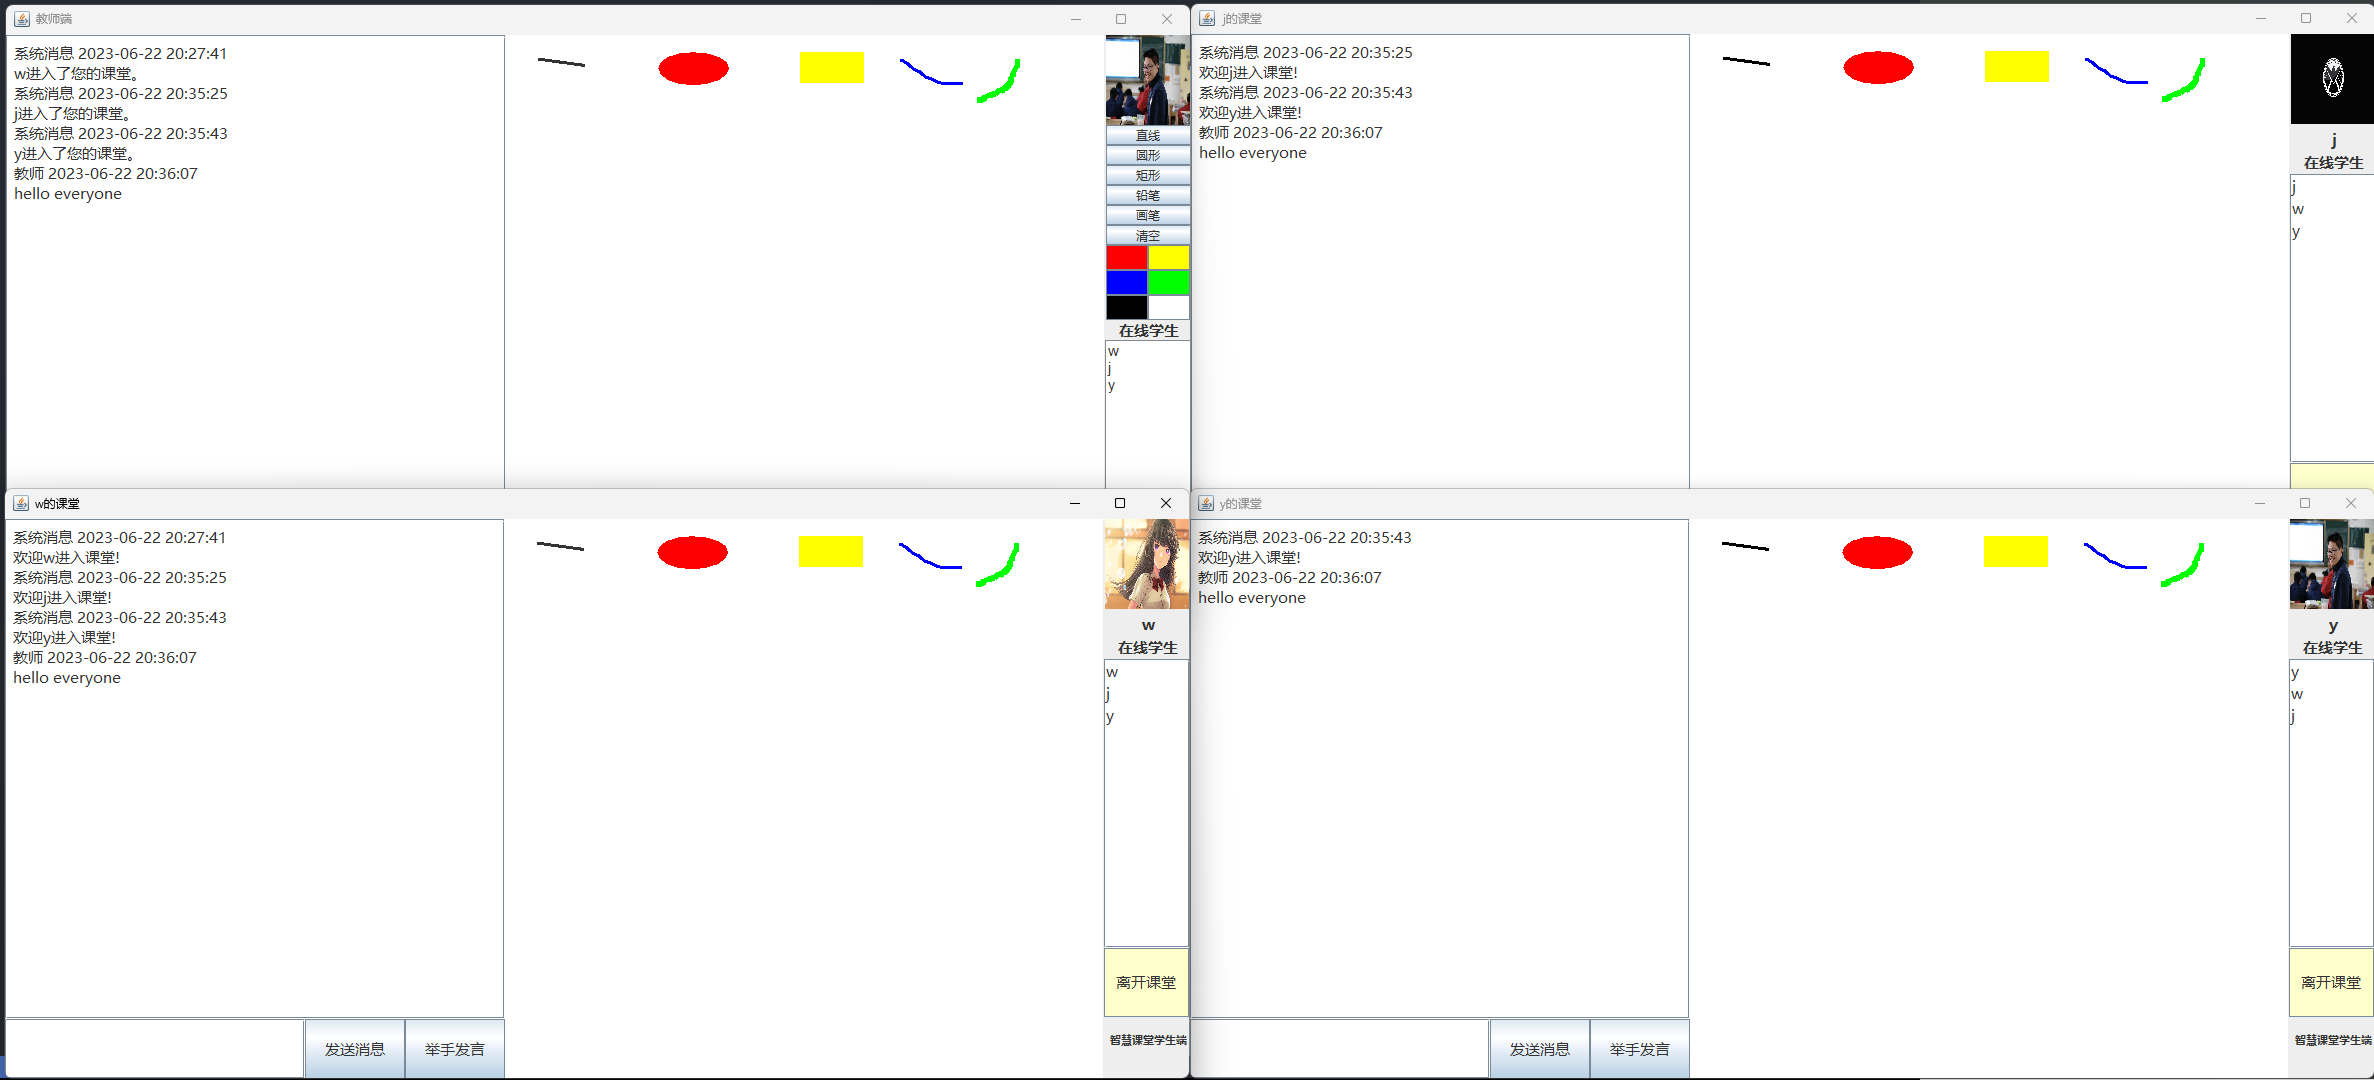
\includegraphics[width=0.9\textwidth]{img/33.png}
    \caption{画板绘图结果}
\end{figure}

\subsection{教师端发送群发信息}
\begin{figure}[htbp]
    \centering
    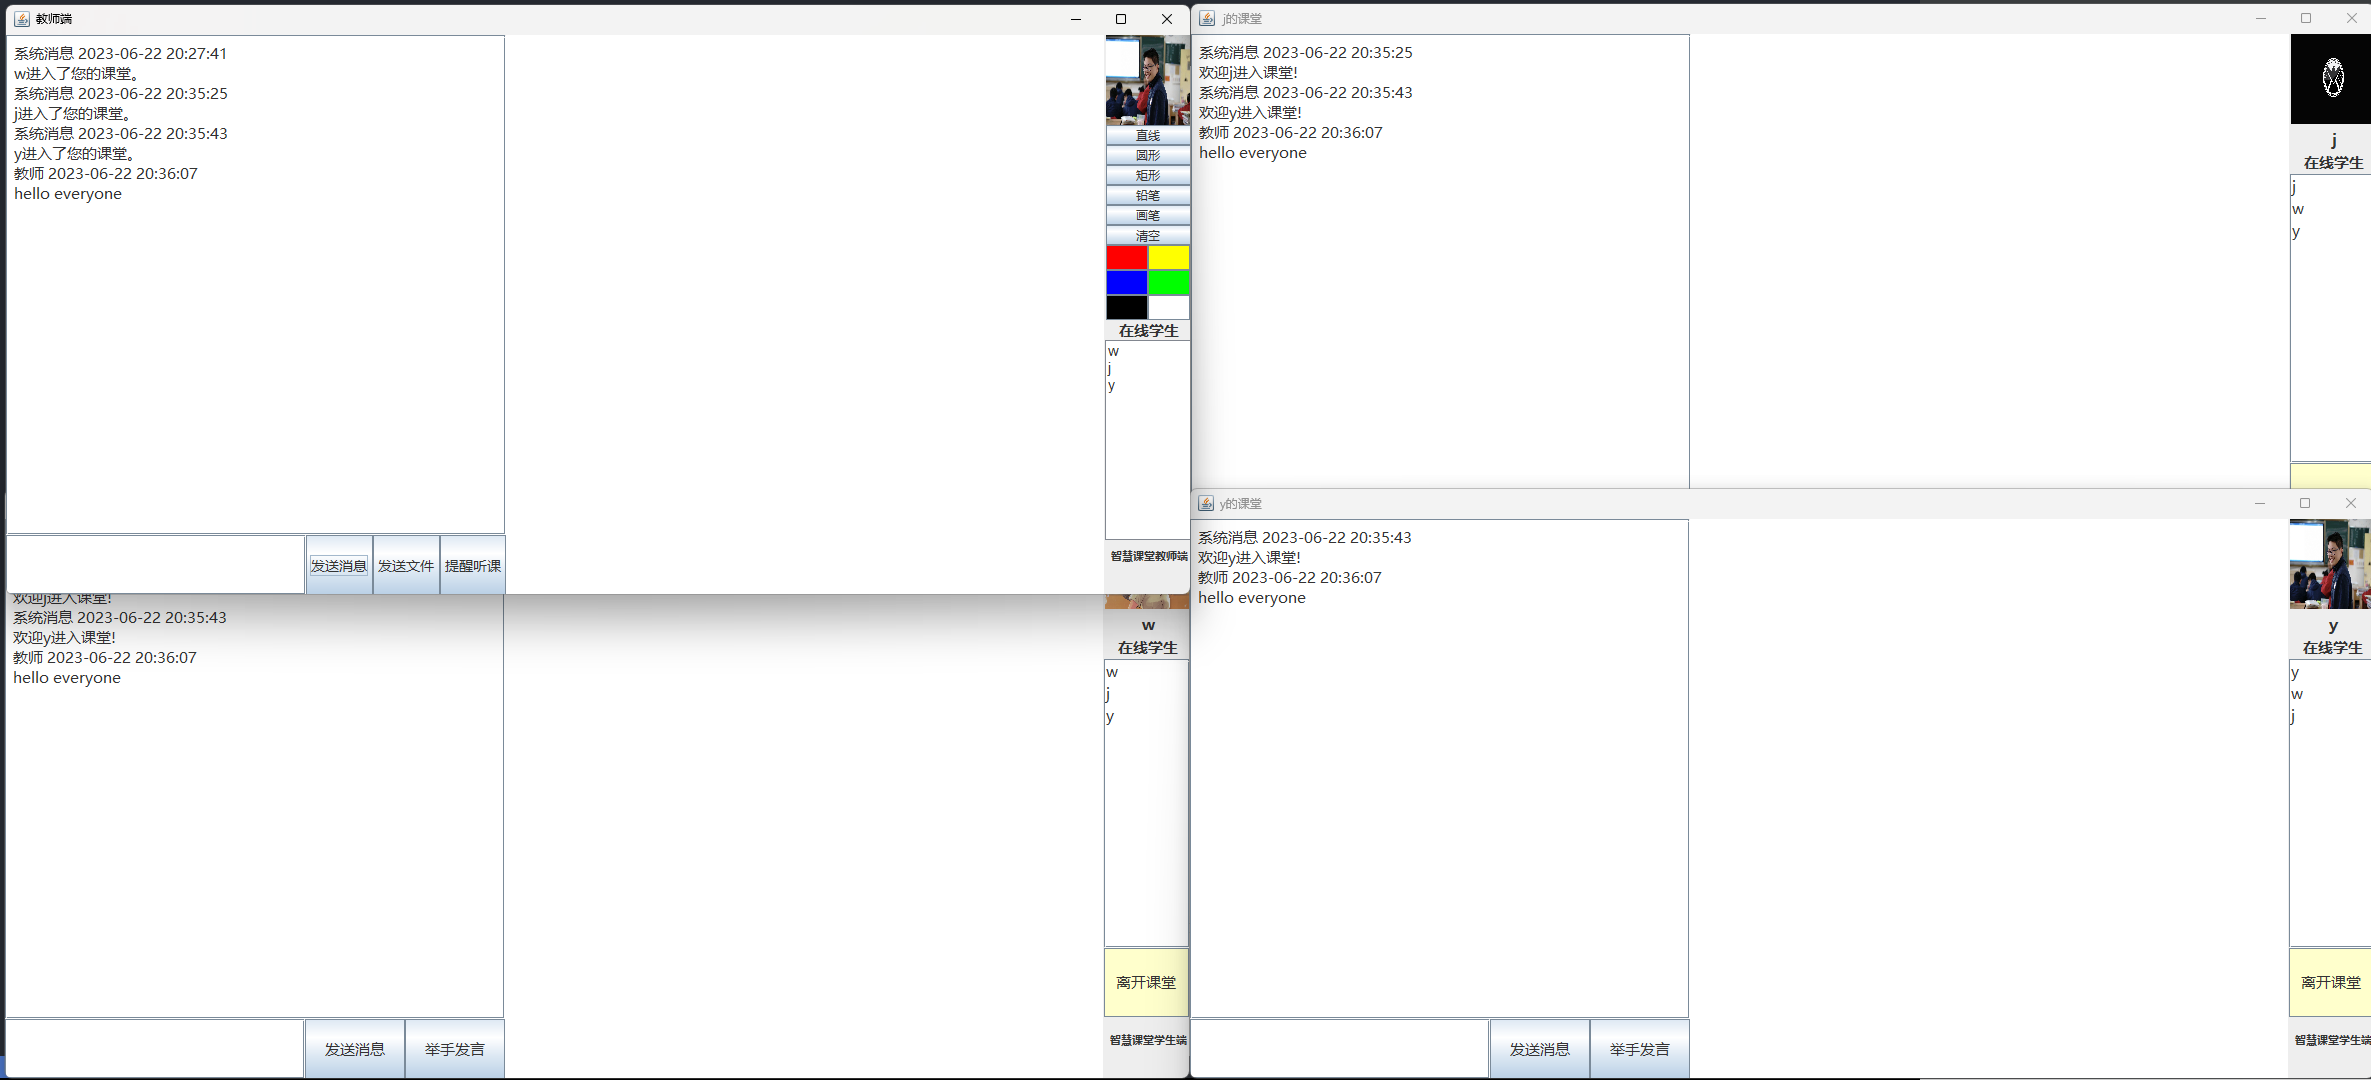
\includegraphics[width=0.9\textwidth]{img/34.png}
    \caption{教师端发送群发信息}
\end{figure}

\newpage

\subsection{学生端发送群发信息}
\begin{figure}[htbp]
    \centering
    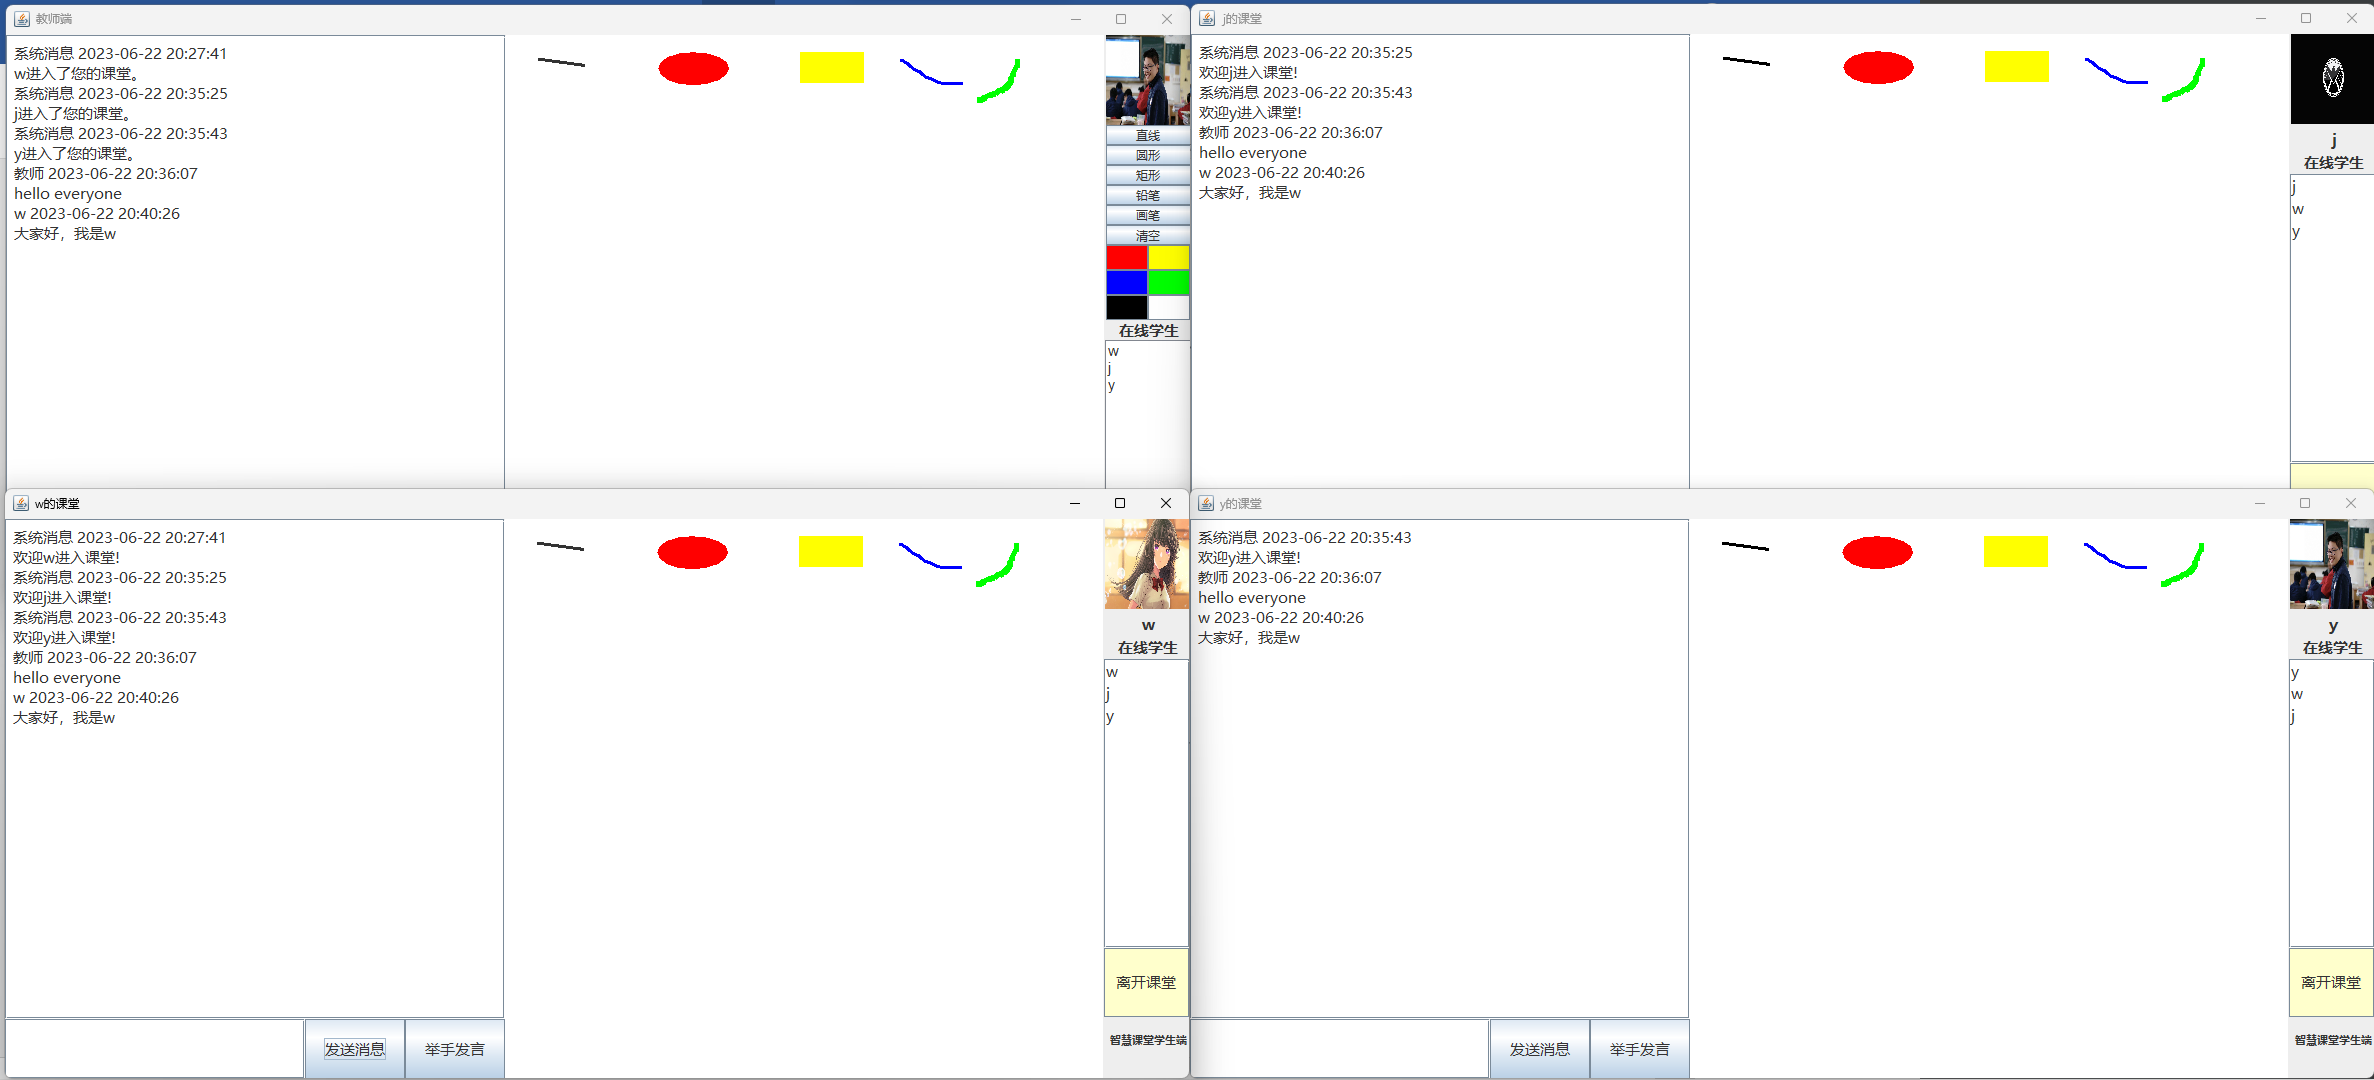
\includegraphics[width=0.9\textwidth]{img/35.png}
    \caption{学生端发送群发信息}
\end{figure}

\subsection{学生端请求发言}
\begin{figure}[htbp]
    \centering
    \begin{minipage}{0.49\textwidth}
        \centering
        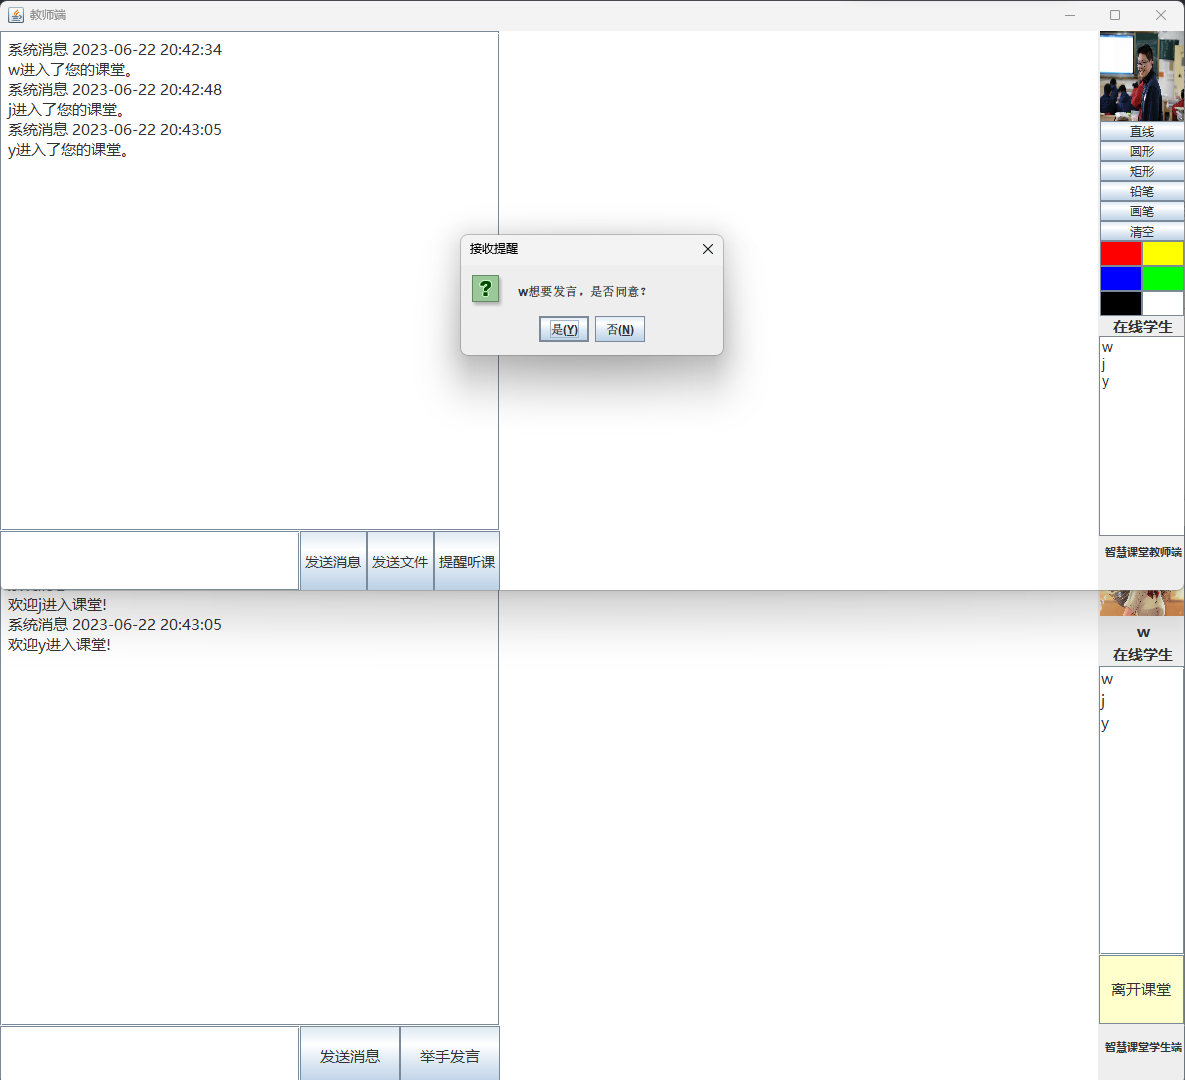
\includegraphics[width=1.0\textwidth]{img/36.png}
    \end{minipage}
    \begin{minipage}{0.49\textwidth}
        \centering
        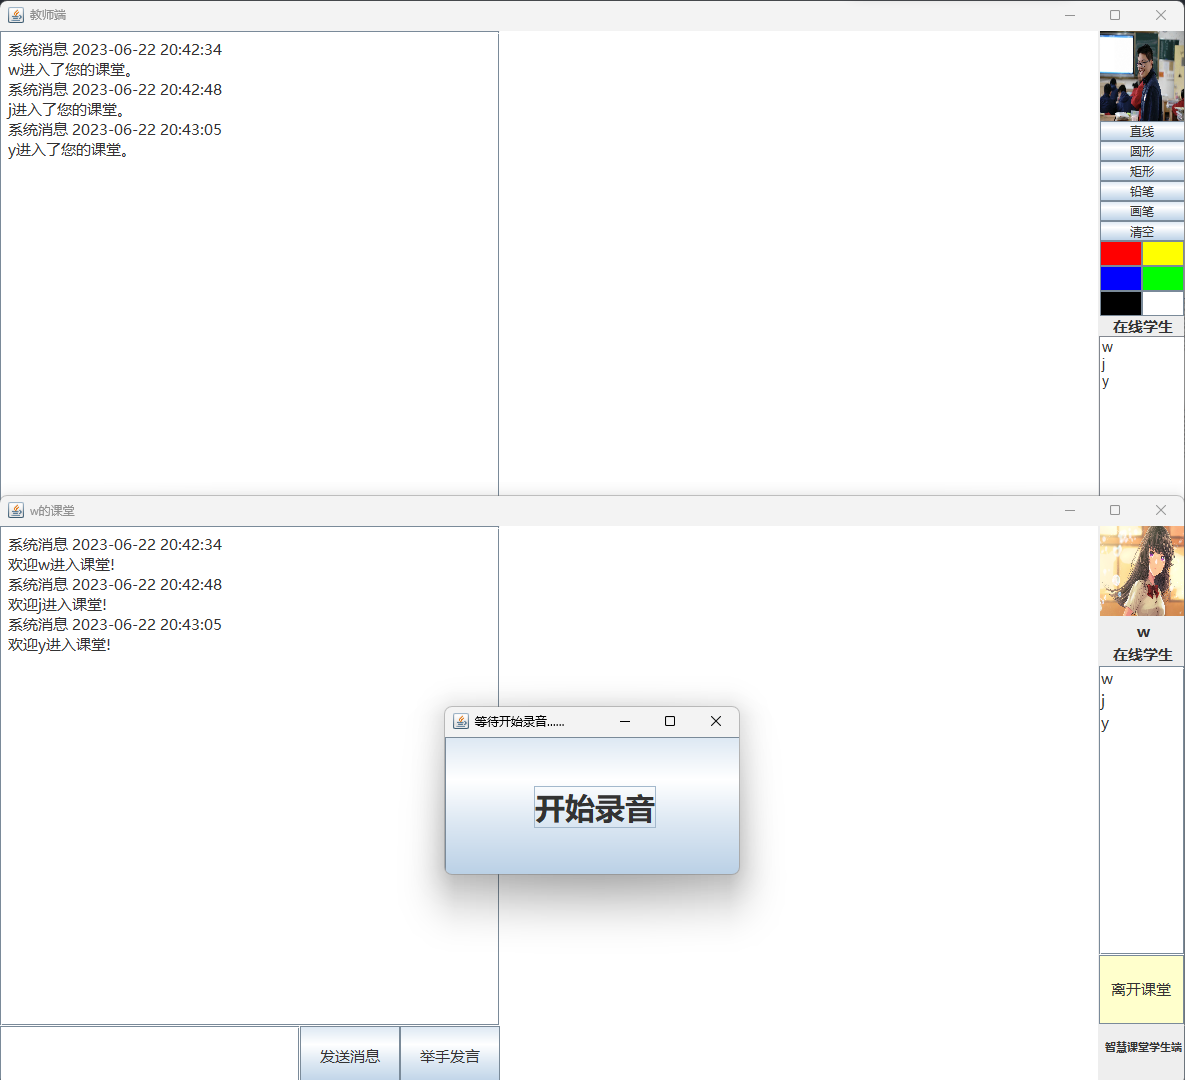
\includegraphics[width=1.0\textwidth]{img/37.png}
    \end{minipage}
    \caption{教师端同意请求}
\end{figure}

\newpage

\subsection{教师端发送文件}
\begin{figure}[htbp]
    \centering
    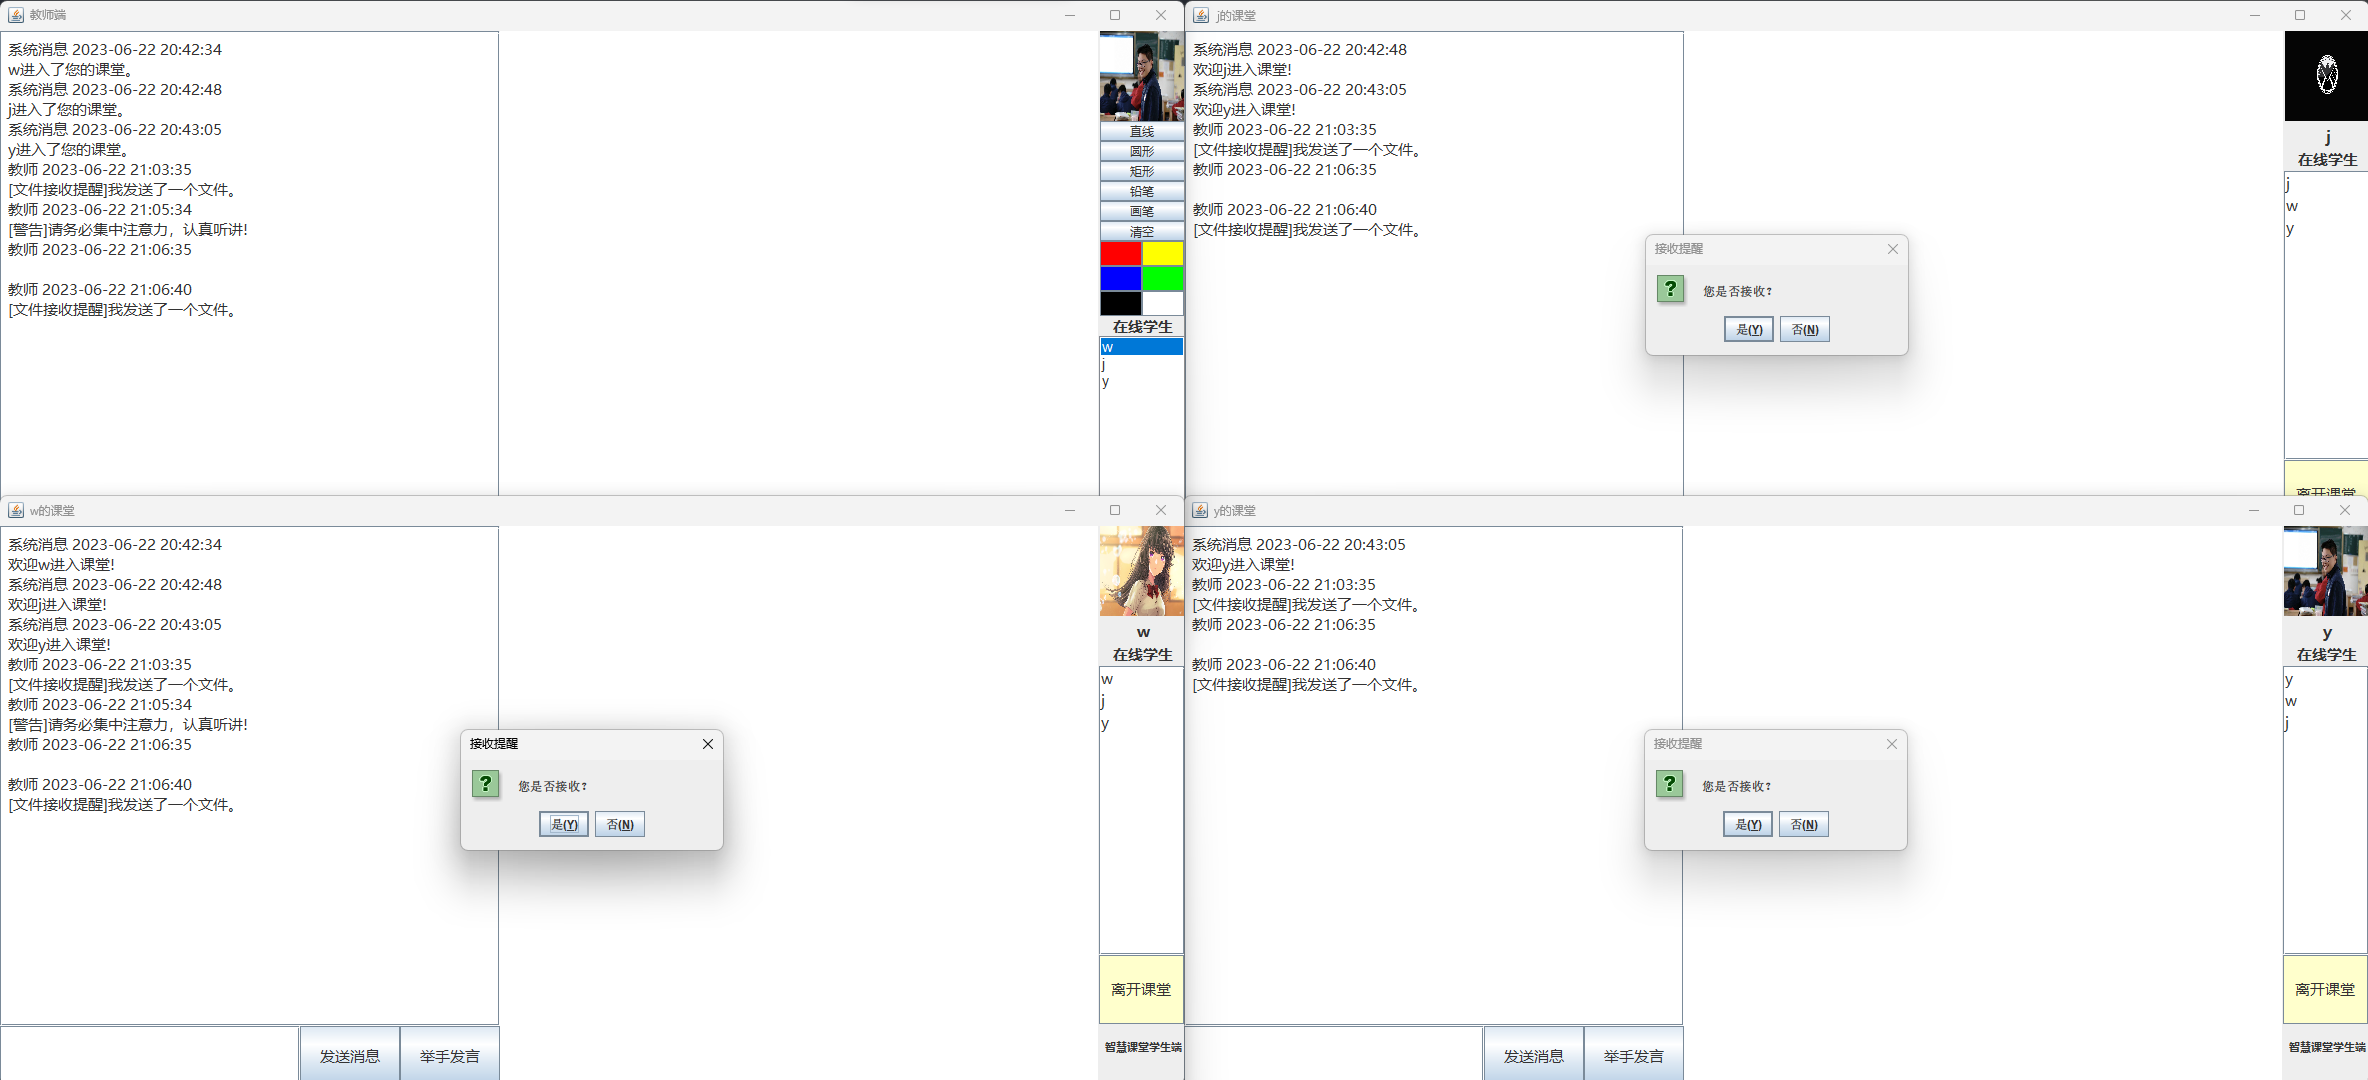
\includegraphics[width=0.9\textwidth]{img/39.png}
    \caption{教师端发送文件}
\end{figure}

\subsection{教师端提醒认真上课}
\begin{figure}[htbp]
    \centering
    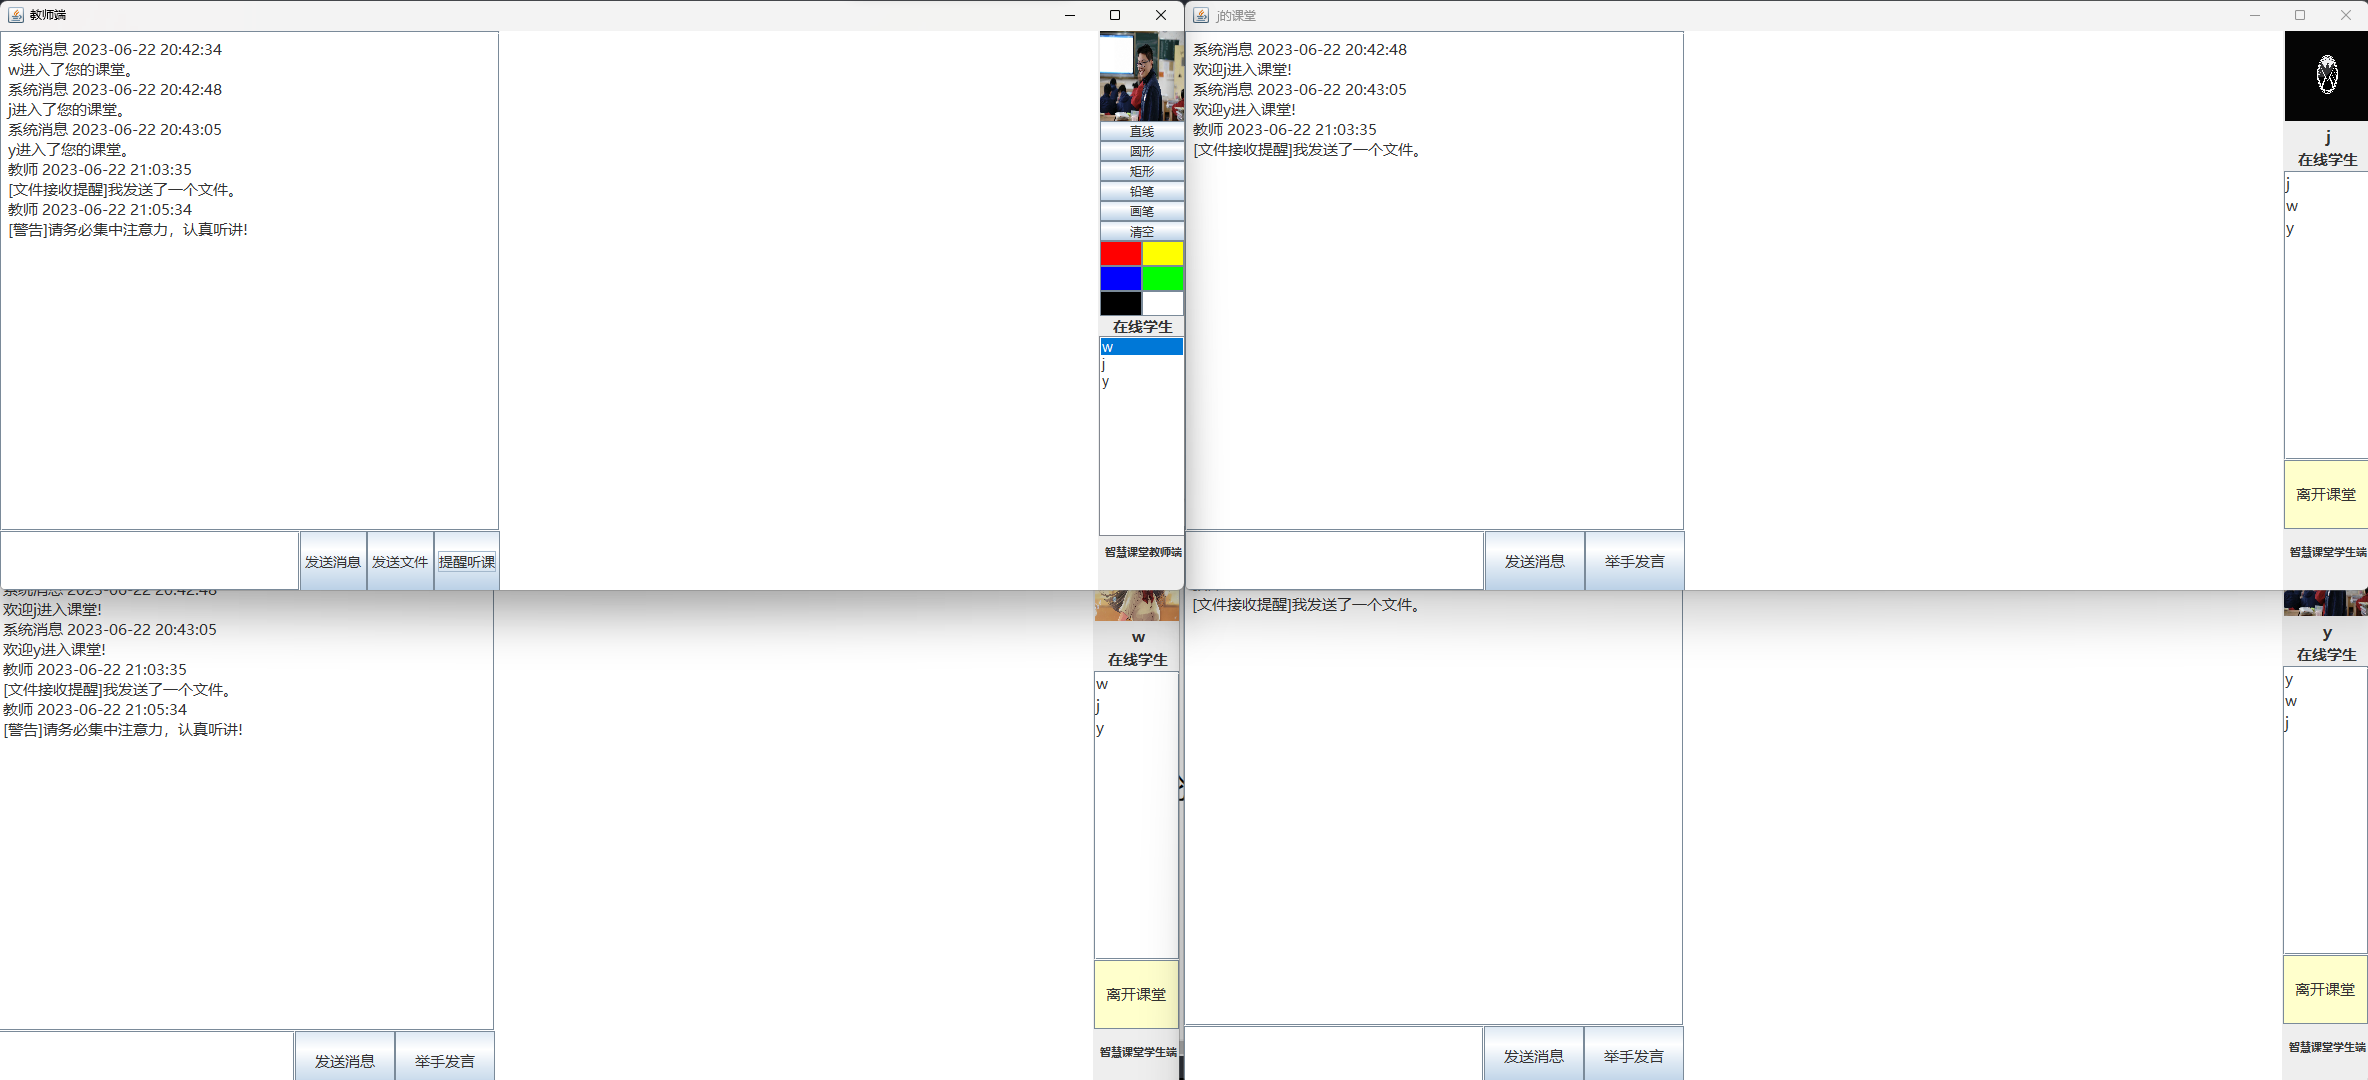
\includegraphics[width=0.9\textwidth]{img/38.png}
    \caption{教师端提醒认真上课}
\end{figure}

\subsection{学生端离开课堂}
\begin{figure}[htbp]
    \centering
    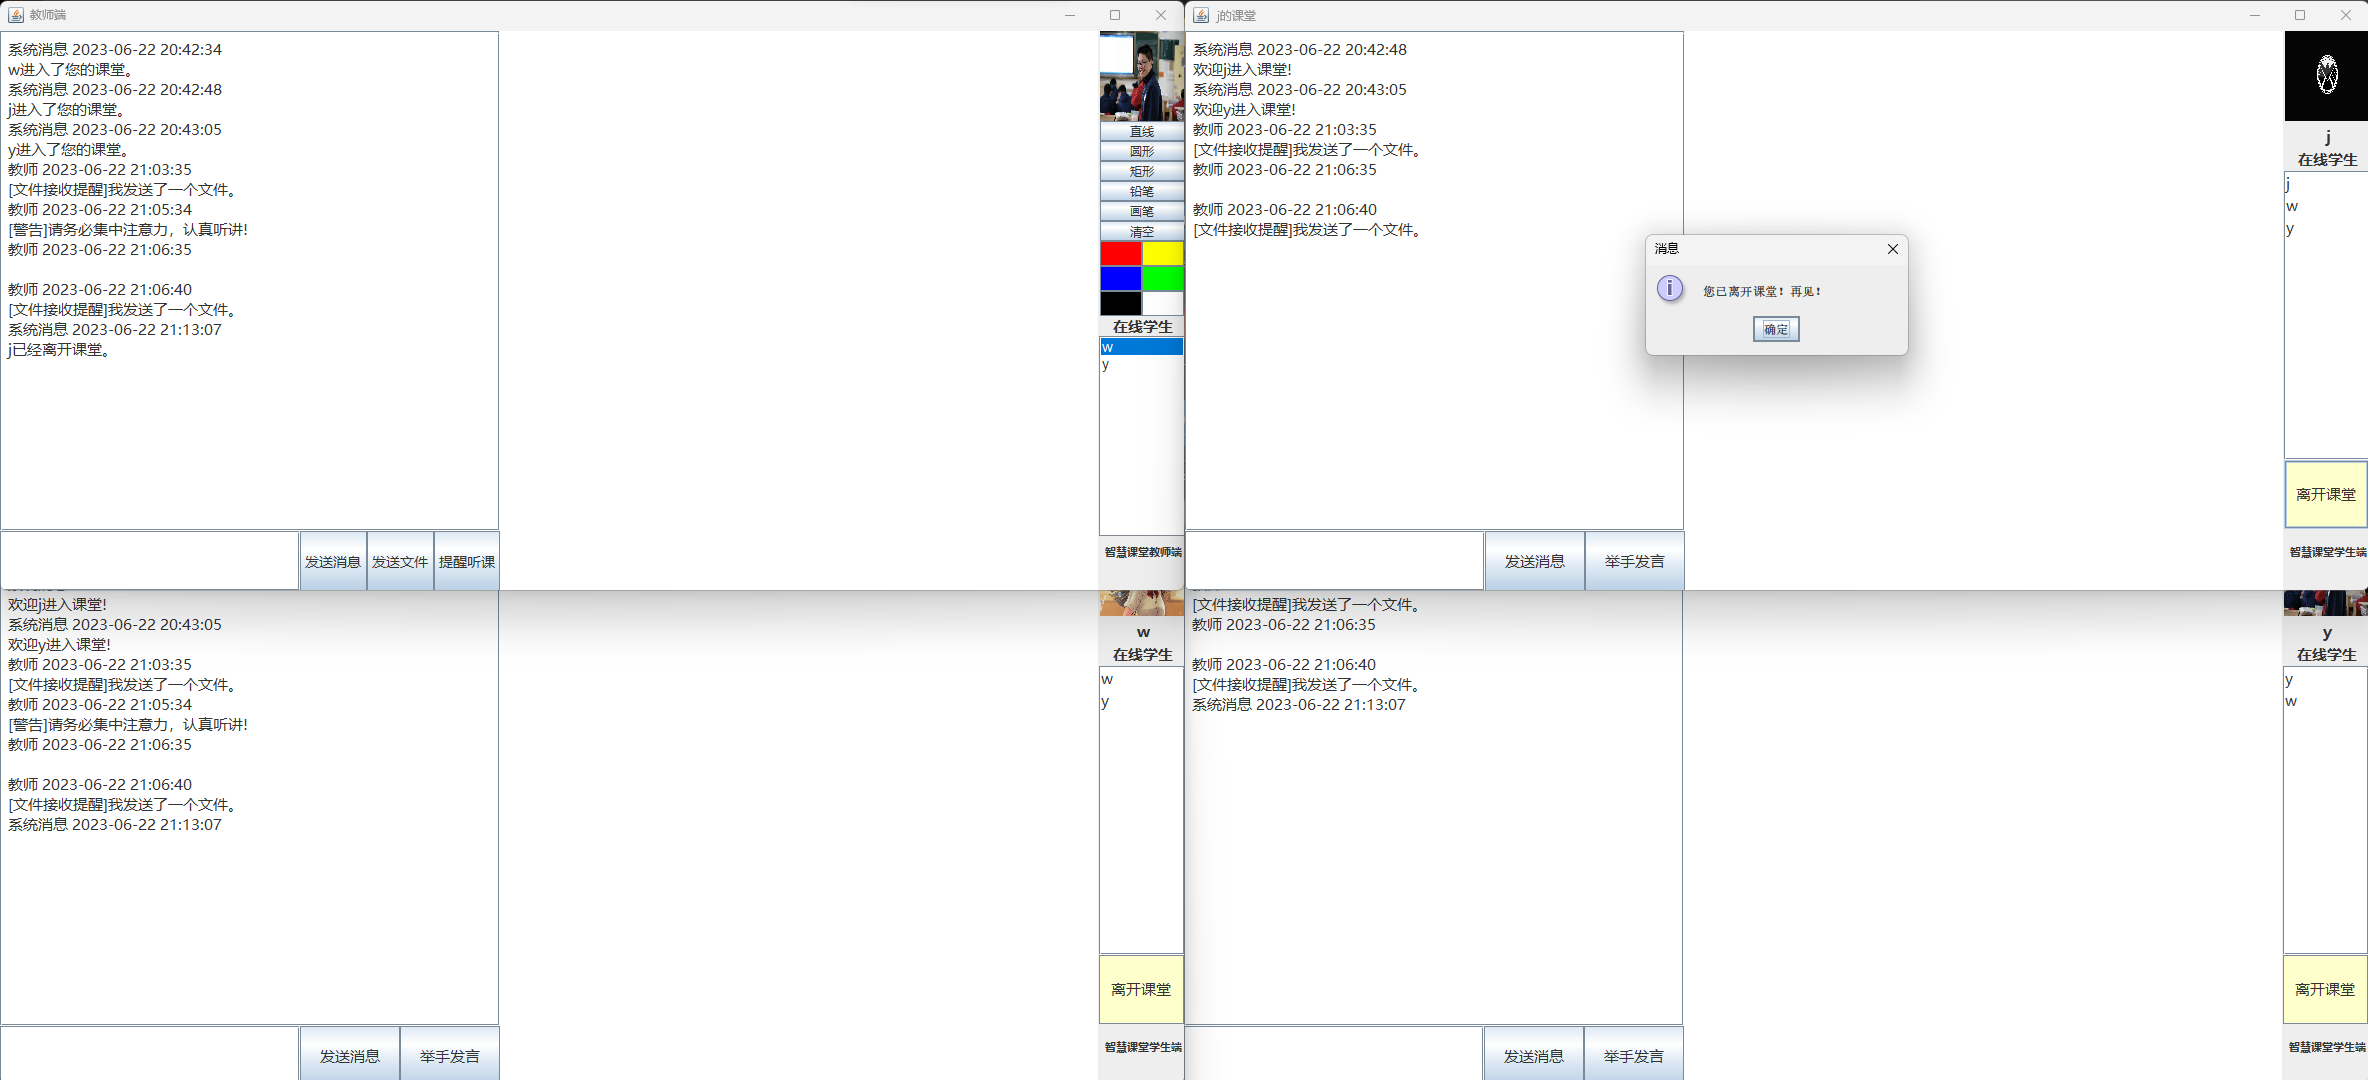
\includegraphics[width=0.9\textwidth]{img/40.png}
    \caption{学生端离开课堂}
\end{figure}

\subsection{教师端最终界面}
\begin{figure}[htbp]
    \centering
    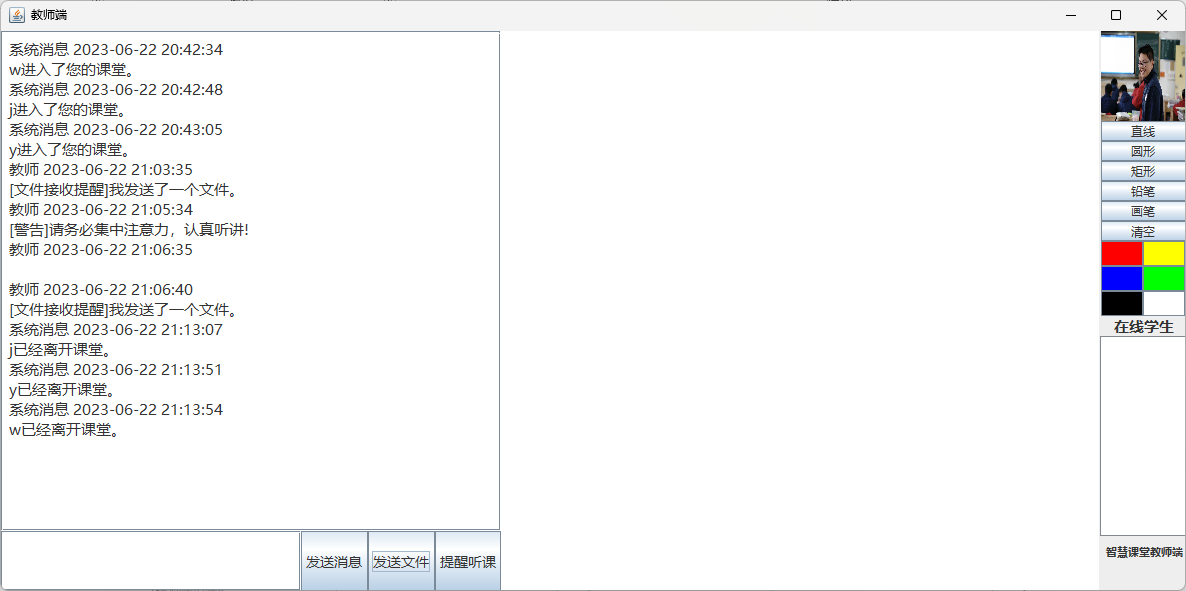
\includegraphics[width=0.9\textwidth]{img/41.png}
    \caption{教师端最终界面}
\end{figure}

\newpage

\section{结论与心得}
\subsection{结论}
本次应用基础实践中,分别实现了一个聊天室程序,并在聊天室的基础上,增加画板功能,实现了一个白板程序。

\subsubsection{聊天室程序测试分析}
\begin{itemize}
    \item 正确性:能够正确的实现客户端和服务器的通信,可以实现不同客户端群聊、私聊的功能,可以正确处理发送文字、发送语音、发送文件等场景需求,以及私聊间窗口抖动的功能。本系统具备正确性。
    \item 健壮性:系统实现了对异常操作的处理。若前端输入非法或未定义的信息,不会影响程序其他功能的正常运行。本系统具备健壮性。
\end{itemize}

\subsubsection{白板程序测试分析}
\begin{itemize}
    \item 正确性:能够正确的实现教师端和学生端的通信,可以实现教师端与学生端进行课堂交互所需的文字提问、语音提问、文件传输、画板绘制、同步画板信息等场景需求。本系统具备正确性。
    \item 健壮性:系统实现了对异常操作的处理。若前端输入非法或未定义的信息,不会影响程序其他功能的正常运行。本系统具备健壮性。
\end{itemize}

\subsection{心得}
写Java聊天室程序和白板程序是一项挑战性的任务。这些程序不仅要求熟悉Java编程语言和相关的库和框架,还需要理解网络编程和并发编程的概念。以下是我在编写这些程序时的一些心得:

1. 网络编程基础:聊天室程序和白板程序都是基于网络的应用程序,所以理解网络编程是非常重要的。需要了解Socket编程、服务器和客户端之间的通信等基本概念。Java提供Socket能够帮助建立网络连接和进行数据传输。

2. 并发编程:在聊天室程序和白板程序中,很可能同时有多个用户进行操作和发送消息。因此,并发编程是必不可少的。Java提供了多线程和线程池等机制来支持并发编程。需要合理地管理线程,确保线程安全和避免竞态条件。

3. 客户端-服务器模型:聊天室程序和白板程序都是基于客户端-服务器模型的应用。服务器负责接收客户端的请求,并将数据转发给其他客户端。客户端负责与服务器建立连接,并发送消息或者接收其他用户的消息。

4. 用户界面设计:聊天室程序和白板程序的用户界面是用户与程序进行交互的重要组成部分。使用Java提供的图形界面库swing来设计用户界面。合理地组织界面元素、响应用户的操作,并实时更新界面显示的数据是至关重要的。

5. 数据传输和存储:在聊天室程序中,消息需要在客户端和服务器之间进行传输。你可以使用数据流进行传输,也可以使用对象序列化等方式。同时白板的实时呈现要求不能简单地发送图片,而是将画图数据抽象化,将画图数据发送给客户端,客户端再根据画图数据进行绘制。

6. 安全性考虑:在设计聊天室程序和白板程序时,要注意安全性问题。对用户进行身份验证和授权,防止未经授权的用户访问和操作系统是很重要的。

7. 测试和调试:编写这些程序后,进行充分的测试和调试是必不可少的。确保程序在各种场景下都能正常运行,并且具备足够的健壮性和容错性。

总结来说,编写Java聊天室程序和白板程序让我的java编程能力得到了很大的提升,也让我对网络编程和并发编程有了更深入的理解。在编写这些程序时,我遇到了很多问题,但是通过查阅资料和与同学的讨论,我都一一解决了。这些程序的编写让我受益匪浅,我相信这些经验会对我今后的学习和工作都有很大的帮助。


\end{document}